% !TEX TS-program = lualatex
% !TEX encoding = UTF-8

\documentclass[12pt]{article} % use larger type; default would be 10pt

% usual packages loading:
\usepackage{forloop}
\usepackage{calc}
\usepackage{fontspec}
\usepackage{graphicx} % support the \includegraphics command and options
\usepackage{geometry} % See geometry.pdf to learn the layout options. There are lots.
\geometry{a4paper} % or letterpaper (US) or a5paper or....
\usepackage[allowdeprecated=false]{gregoriotex} % for gregorio score inclusion
\usepackage{fullpage} % to reduce the margins
\usepackage{titlesec}
%\usepackage{bold-extra}
\usepackage[oldstyle]{libertine}
\usepackage{lettrine}
\setlength{\parindent}{-0.25in}

% Repeat something:
\newcounter{loopcntr}
\newcommand{\repeatthing}[2][1]{%
  \forloop{loopcntr}{0}{\value{loopcntr}<#1}{#2}%
}

% STYLE FOR THE TITLE PAGE
\usepackage{fancyhdr}
\pagestyle{fancy}
\lhead{}
\chead{\color{benblue1}{ \repeatthing[17]{\greornamentation{2}{12}} }}
\rhead{}
\lfoot{}
\cfoot{\color{benblue1}{ \repeatthing[17]{\greornamentation{2}{12}} }\\ \color{black}\thepage}
\rfoot{}
\renewcommand{\headrulewidth}{0pt}
\setlength{\headsep}{25pt}

 
%eso-pic package stuff for placing something at specific coordinates on the page
\newcommand{\placetextbox}[3]{% \placetextbox{<horizontal pos>}{<vertical pos>}{<stuff>}
  \setbox0=\hbox{#3}% Put <stuff> in a box
  \AddToShipoutPictureFG*{% Add <stuff> to current page foreground
    \put(\LenToUnit{#1\paperwidth},\LenToUnit{#2\paperheight}){\vtop{{\null}\makebox[0pt][c]{#3}}}%
  }%
}%

% REDS
\definecolor{benred1}{HTML}{E73930}
\definecolor{benred2}{HTML}{AD1E0E}
\definecolor{benred3}{HTML}{EA4031}
\definecolor{benred4}{HTML}{E9432D}
\definecolor{benred5}{HTML}{B22312}
\definecolor{benred6}{HTML}{EE4F31}
\definecolor{benred7}{HTML}{C4160D}
\definecolor{benred8}{HTML}{E82C00} %seems good, maybe the best?
\definecolor{benred9}{HTML}{FF3100} %seems good
\definecolor{benred10}{HTML}{FF5000}
\definecolor{benred11}{HTML}{F53000} %seems good
\definecolor{benred12}{HTML}{F53010} %seems good, maybe the best?

% BLUES
\definecolor{benblue1}{HTML}{2B22C7}

% YELLOWS
\definecolor{benyellow1}{HTML}{FFD435}
\definecolor{benyellow2}{HTML}{7C6F3B}

% DEFINE THE FORMATTING OF
% PSALM TEXT
\newenvironment{psalmtext}{\leftskip 0.25in}{\vspace{2 mm}}
\newenvironment{rubric}{\color{benred8} \itshape \leftskip 0in \setlength{\parindent}{0.25in}}{\vspace{2 mm}}
\newenvironment{response}{\leftskip 0in \setlength{\parindent}{0in}}{\vspace{2 mm}}

% REDUCES SUBSECTION SPACE
\def\subspace{\vspace{-13 mm}}

% MAKES Flexa : TEXT
\def\flex{\textit{\textcolor{benred8}{Flexa :}}}

% MAKES Cantor : TEXT
\def\cantor{\textit{\textcolor{benred8}{Cantor :}}}

% MAKES vel : TEXT
\def\vel{\textit{\textcolor{benred8}{vel :}}}

% MAKES deinde : TEXT
\def\deinde{\textit{\textcolor{benred8}{deinde :}}}

% MAKES Repetitur : TEXT
\def\repetitur{\textit{\textcolor{benred8}{Repetitur :}}}

% MAKES secreto usque ad TEXT
\def\secreto{\textit{\textcolor{benred8}{secreto usque ad}}}

% MAKES T.P. TEXT
\def\TemporePaschale{\textit{\textcolor{benred8}{T. P.}}}

% MAKES ALL \GreStars RED
\let\OldGreStar\GreStar
\renewcommand{\GreStar}{\textcolor{benred8}{\OldGreStar}}

% MAKES ALL \GreDaggers RED
\let\OldGreDagger\GreDagger
\renewcommand{\GreDagger}{\textcolor{benred8}{\OldGreDagger}}

% MAKES ALL \Vbars RED
\let\oldVbar\Vbar
\def\VVbar{\textcolor{benred8}{\oldVbar\oldVbar .}}
\renewcommand{\Vbar}{\textcolor{benred8}{\oldVbar .}}

% MAKES ALL \Rbars RED
\let\oldRbar\Rbar
\renewcommand{\Rbar}{\textcolor{benred8}{\oldRbar .}}

% MAKES ALL \Abars RED
\let\oldAbar\Abar
\renewcommand{\Abar}{\textcolor{benred8}{\oldAbar .}}

% MAKES ALL \grealtcrosses RED
\let\oldgrealtcross\grealtcross
\renewcommand{\grealtcross}{\textcolor{benred8}{\oldgrealtcross}}

% ANOTHER CROSS GLYPH USED FOR THE SIGN OF THE CROSS WITH THUMB ON CHEST
\newcommand{\grebencross}{\fontspec{gresym3.ttf}\textcolor{benred8}{T}}


% FORMAT SECTIONS - use titlesec package
\titleformat{\section}{\centering\scshape\Huge\color{benred8}}{}{1em}{}

% REDUCES SUBSECTION SPACE
%\def\subspace{\vspace{-13 mm}}
%\def\subspace{\vspace{0 mm}}
\titleformat{\subsection}{\normalfont}{}{1em}{}[\vspace{-5 mm}]
\titlespacing{\subsection}{0 mm}{0 mm}{0 mm}

% FORMAT SUBSUBSECTIONS - use titlesec package
\titleformat{\subsubsection}{\centering\normalfont\color{benred8}}{}{1em}{}
\titlespacing{\subsubsection}{0 mm}{0 mm}{0 mm}

% SPACE BETWEEN Capitulum AND BIBLE VERSE
\def\capitulumSpace{\hspace{20 mm}}

% ANNOTATION STYLE
\grechangestyle{annotation}{\small\scshape\bfseries\color{benred8}}
\grechangedim{annotationraise}{-3 mm}{scalable}


%%%%%%%%%%%%%%%%%%%%%%%%%%%%
% HERE BEGINS THE DOCUMENT %
%%%%%%%%%%%%%%%%%%%%%%%%%%%%

\begin{document}

\pagenumbering{gobble}

\vspace*{35 pt}

\begin{center}

\color{benred8}

{\fontsize{2.660cm}{5 em}\selectfont

PSALTERIUM

}

\vspace*{15 pt}

{\fontsize{2.975cm}{5 em}\selectfont

VESPERALE

}

\vspace*{20 pt}

{\fontsize{1.5cm}{1 em}\selectfont

JUXTA RITUM

\vspace*{2.7 mm}

ROMANUM

\vspace*{5 mm}

ANTIQUIOREM

}

\vspace*{10 mm}

\begin{Huge}

ANNOTATUM

\end{Huge}\begin{Large}

ATQUE

\vspace*{-1.0 mm}

\end{Large}\begin{Huge}

ORNATUM SIGNIS RHYTHMICIS

\end{Huge}

\vspace*{3 mm}

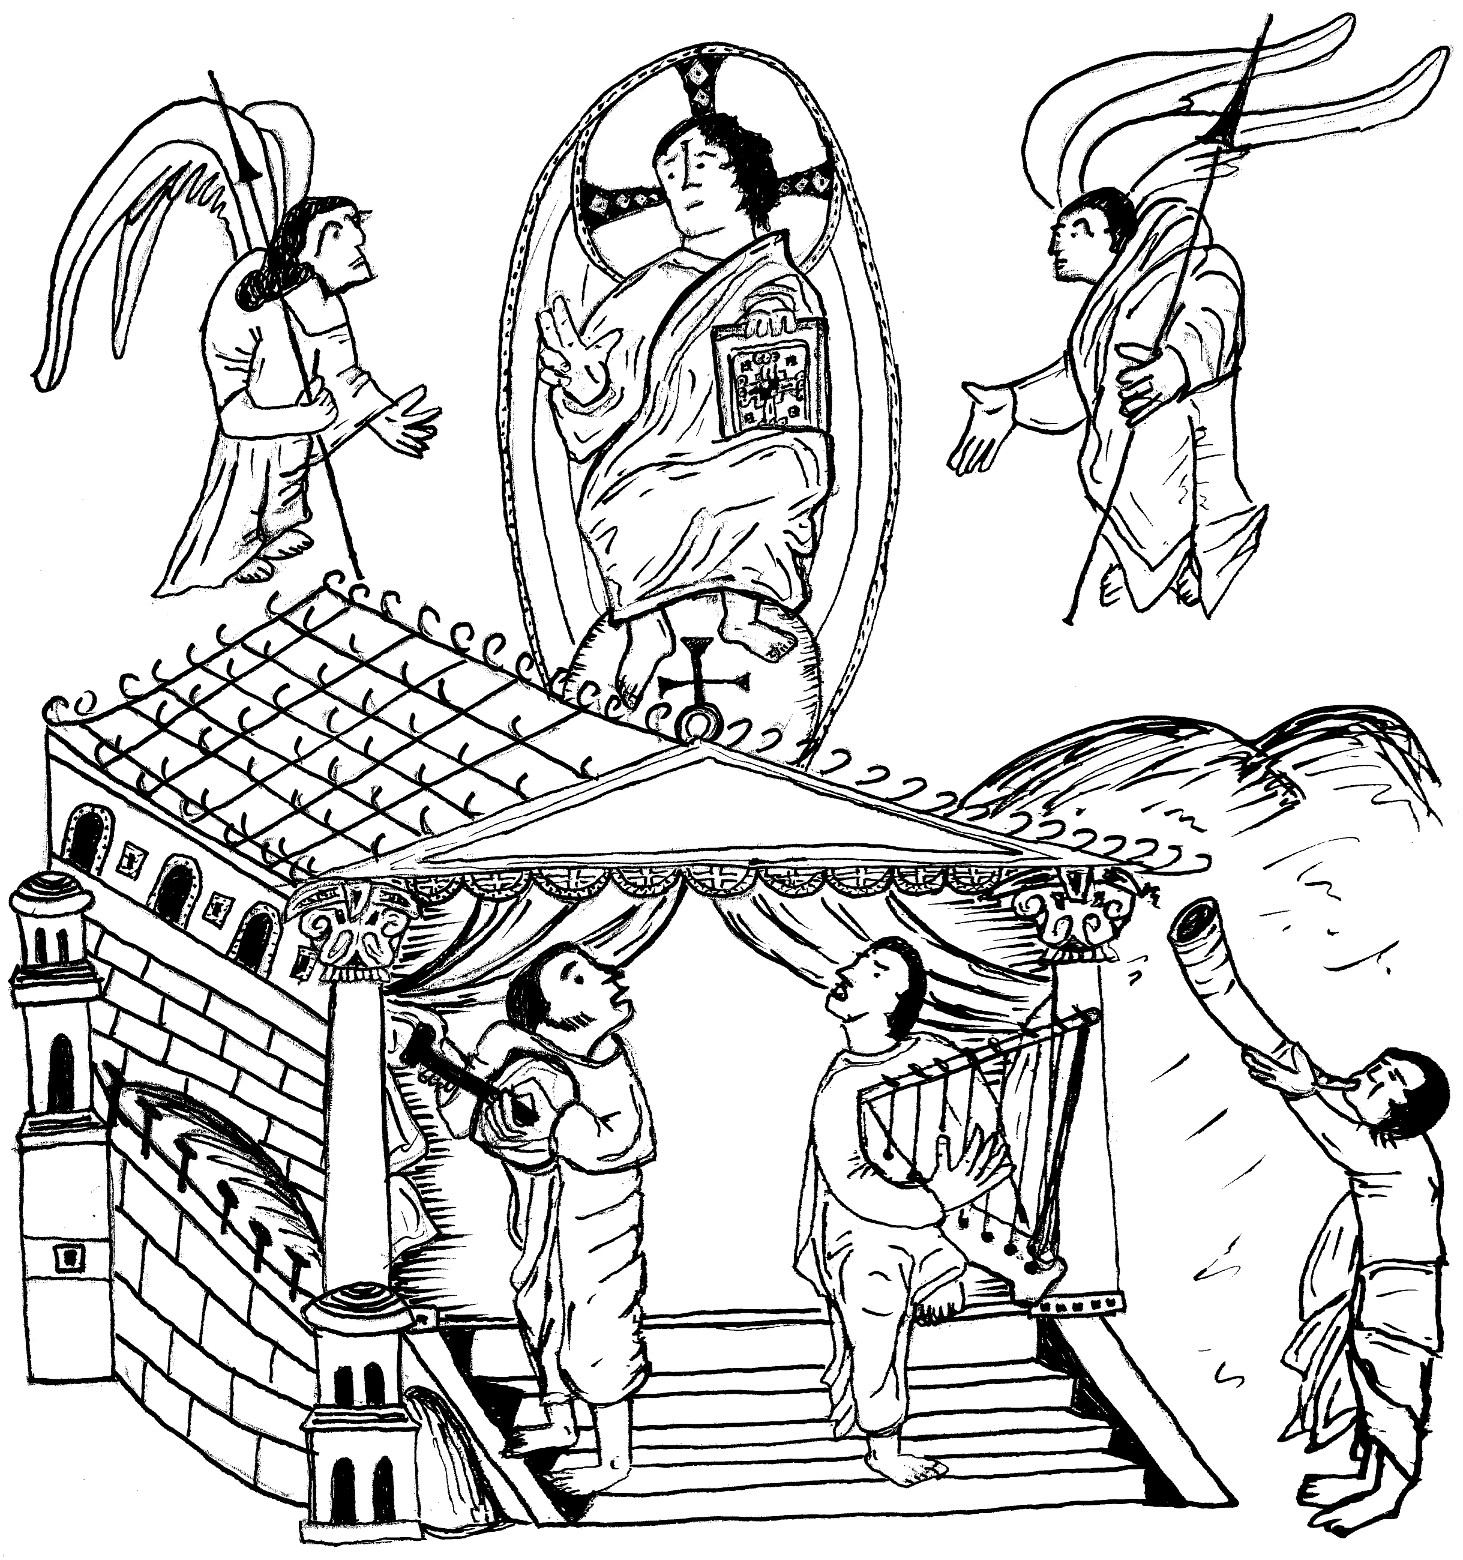
\includegraphics[height=7.06cm]{CoverImage02_s.png}

\vspace*{3 mm}

\begin{large}

\textsc{Versio 2.0 MMXVII}

\end{large}

\end{center}

%redefine 'plain' page style to have blue page numbers too
\fancypagestyle{plain}{
    \chead{}
    \cfoot{\textcolor{benblue1}{\thepage}}

}

\newpage
\thispagestyle{empty}
\mbox{}
\newpage
\chead{\color{benred8}\textsc{Dominica}}
\cfoot{\textcolor{benblue1}{\thepage}}
\thispagestyle{plain}
\pagenumbering{arabic}  
\setcounter{page}{3}

\begin{center}\begin{Huge}\textsc{\textcolor{benred8}{Dominica ad Vesperas}}\end{Huge}\end{center}

\begin{center}Pater no\libertineGlyph{s_t}er. Ave Mar\'{i}a.\end{center}

\grechangestyle{initial}{\fontsize{43}{43}\selectfont}
\greannotation{\upshape\Vbar}
\gregorioscore[a]{DeusInAdjutorium.gtex}

\begin{rubric}
A Septuagesima usque ad Pascha, loco \emph{\textcolor{black}{Allelúia}}, canitur :

\end{rubric}

\gregorioscore[a]{LausTibi.gtex}

\vspace{-0.10in}

\begin{center}\begin{large}\textbf{\textsc{\textcolor{benred8}{1 Antiphona. VII c 2}}}\end{large}\end{center}

\vspace{-0.10in}

{\gresetinitiallines{2}
\grechangestyle{initial}{\fontsize{160}{160}\selectfont}
\gregorioscore[a]{Dominica/DomAnt1-01.gtex}

}

\vspace{-0.125in}

{
\centering
\textcolor{benred8}{Psalmus 109.}

}

\begin{psalmtext}
Donec ponam ini\textbf{mí}cos \textbf{tu}os, \GreStar\ scabéllum \textbf{pe}dum tu\textbf{ó}rum.

Virgam virtútis tuæ emíttet Dómi\textbf{nus} ex \textbf{Si}on : \GreStar\ domináre in médio inimi\textbf{có}rum tu\textbf{ó}rum.

Tecum princípium in die virtútis tuæ in splendóri\textbf{bus} sanc\textbf{tó}rum : \GreStar\ ex útero ante lucíferum \textbf{gé}nu\textbf{i} te.

Jurávit Dóminus et non pæni\textbf{té}bit \textbf{e}um : \GreStar\ Tu es sacérdos in æt\'{e}rnum secúndum órdi\textbf{nem} Mel\textbf{chí}sedech.

Dóminus a \textbf{dex}tris \textbf{tu}is, \GreStar\ confrégit in die iræ \textbf{su}æ \textbf{re}ges.

Judicábit in natiónibus, im\textbf{plé}bit ru\textbf{í}nas : \GreStar\ conquassábit cápita in \textbf{ter}ra mul\textbf{tó}rum.

De torrénte in \textbf{vi}a \textbf{bi}bet : \GreStar\ proptérea exal\textbf{tá}bit \textbf{ca}put.

Glória \textbf{Pa}tri, et \textbf{Fí}lio, \GreStar\ et Spi\textbf{rí}tui \textbf{Sanc}to.

Sicut erat in princípio, et \textbf{nunc}, et \textbf{sem}per, \GreStar\ et in sǽcula sæcu\textbf{ló}rum. \textbf{A}men.

\end{psalmtext}

\gregorioscore[a]{Dominica/DomAnt1-02.gtex}

\vspace{2 mm}

%% DOMINICA 2 ANT.

\subsection*{}

\greannotation{2 {\upshape\Abar} IV g}
\gregorioscore[a]{Dominica/DomAnt2-01.gtex}

{
\centering
\textcolor{benred8}{Psalmus 110.}

}

\gregorioscore[a]{Dominica/DomFL2.gtex}


\begin{psalmtext}
Magna ó\emph{pera} \textbf{Dó}mini : \GreStar\ exquisíta in omnes voluntátes \textbf{e}jus.

Conféssio et magnificéntia \emph{opus} \textbf{e}jus : \GreStar\ et ju\libertineGlyph{s_t}ítia ejus manet in sǽculum \textbf{sǽ}culi.

Memóriam fécit mirabílium suórum, \GreDagger\ miséricors et mise\emph{rátor} \textbf{Dó}minus : \GreStar\ escam dedit timénti\textbf{bus} se.

Memor erit in sǽculum te\libertineGlyph{s_t}a\emph{ménti} \textbf{su}i : \GreStar\ virtútem óperum suórum annuntiábit pópulo \textbf{su}o :

Ut det illis hæredi\emph{tátem} \textbf{gén}tium : \GreStar\ ópera mánuum ejus véritas et ju\textbf{dí}cium.

Fidélia ómnia mandáta ejus : \GreDagger\ confirmáta in sǽ\emph{culum} \textbf{sǽ}culi : \GreStar\ fa\libertineGlyph{c_t}a in veritáte et æqui\textbf{tá}te.

Redemptiónem misit pó\emph{pulo} \textbf{su}o : \GreStar\ mandávit in ætérnum te\libertineGlyph{s_t}améntum \textbf{su}um.

\textcolor{benred8}{\emph{Fit reverentia :}} San\libertineGlyph{c_t}um et terríbile \emph{nomen} \textbf{e}jus : \GreStar\ inítium sapiéntiae timor \textbf{Dó}mini.

Intellé\libertineGlyph{c_t}us bonus ómnibus facién\emph{tibus} \textbf{e}um : \GreStar\ laudátio ejus manet in sǽculum \textbf{sǽ}culi.

Glória Pa\emph{tri, et} \textbf{Fí}lio, \GreStar\ et Spirítui \textbf{Sanc}to.

Sicut erat in princípio, et \emph{nunc, et} \textbf{sem}per, \GreStar\ et in sǽcula sæculórum. \textbf{A}men.

\end{psalmtext}

\gregorioscore[a]{Dominica/DomAnt2-02.gtex}

\vspace{2 mm}

%% DOMINICA 3 ANT.

\subsection*{}

\greannotation{3 {\upshape\Abar} IV a}
\gregorioscore[a]{Dominica/DomAnt3-01.gtex}

%{
%\centering
%\textcolor{benred8}{Psalmus 111.}
%
%}

\subsubsection*{Psalmus 111.}

\gregorioscore[a]{Dominica/DomFL3.gtex}


\begin{psalmtext}
Potens in terra erit \emph{semen} \textbf{e}jus : \GreStar\ generátio re\libertineGlyph{c_t}órum \emph{benedi}\textbf{cé}tur.

Glória et divítiae in \emph{domo} \textbf{e}jus : \GreStar\ et ju\libertineGlyph{s_t}ítia ejus manet in \emph{sǽculum} \textbf{sǽ}culi.

Exórtum e\libertineGlyph{s_t} in ténebris \emph{lumen} \textbf{rec}tis : \GreStar\ miséricors, et mise\emph{rátor, et} \textbf{jus}tus.

Jucúndus homo qui miserétur et cómmodat, \GreDagger\ dispónet sermónes suos \emph{in ju}\textbf{dí}cio : \GreStar\ quia in ætérnum \emph{non commo}\textbf{vé}bitur.

In memória ætérna \emph{erit} \textbf{jus}tus : \GreStar\ ab auditióne ma\emph{la non ti}\textbf{mé}bit.

Parátum cor ejus speráre in Dómino, \GreDagger\ confirmátum \emph{e\libertineGlyph{s_t} cor} \textbf{e}jus : \GreStar\ non commovébitur donec despíciat i\emph{nimícos} \textbf{su}os.

Dispérsit, dedit paupéribus : \GreDagger\ ju\libertineGlyph{s_t}ítia ejus manet in sǽ\emph{culum} \textbf{sǽ}culi : \GreStar\ cornu ejus exaltá\emph{bitur in} \textbf{gló}ria.

Peccátor vidébit, et irascétur, \GreDagger\ déntibus suis fremet \emph{et ta}\textbf{bé}scet : \GreStar\ desidérium pecca\emph{tórum pe}\textbf{rí}bit.

Glória Pa\emph{tri, et} \textbf{Fí}lio, \GreStar\ et Sp\emph{irítui} \textbf{Sanc}to.

Sicut erat in princípio, et \emph{nunc, et} \textbf{sem}per, \GreStar\ et in sǽcula sæ\emph{culórum}. \textbf{A}men.

\end{psalmtext}

\gregorioscore[a]{Dominica/DomAnt3-02.gtex}

\vspace{2 mm}

%% DOMINICA 4 ANT.

\subsection*{}

\greannotation{4 {\upshape\Abar} VII c}
\gregorioscore[a]{Dominica/DomAnt4-01.gtex}

\subsubsection*{Psalmus 112.}

\gregorioscore[a]{Dominica/DomFL4.gtex}

\begin{psalmtext}
\textcolor{benred8}{\emph{Fit reverentia :}} Sit nomen Dómini \textbf{be}ne\textbf{díc}tum, \GreStar\ ex hoc nunc, et \textbf{us}que in \textbf{sǽ}culum.

A solis ortu usque \textbf{ad} oc\textbf{cá}sum, \GreStar\ laudábile \textbf{no}men \textbf{Dó}mini.

Excélsus super omnes \textbf{gen}tes \textbf{Dó}minus, \GreStar\ et super cælos \textbf{gló}ria \textbf{e}jus.

Quis sicut Dóminus Deus no\libertineGlyph{s_t}er, qui in \textbf{al}tis \textbf{há}bitat, \GreStar\ et humília réspicit in cælo \textbf{et} in \textbf{ter}ra?

Súscitans a \textbf{ter}ra \textbf{í}nopem, \GreStar\ et de \libertineGlyph{s_t}ércore \textbf{é}rigens \textbf{páu}perem :

Ut cóllocet eum \textbf{cum} prin\textbf{cí}pibus, \GreStar\ cum princípibus \textbf{pó}puli \textbf{su}i.

Qui habitáre facit \libertineGlyph{s_t}éri\textbf{lem} in \textbf{do}mo, \GreStar\ matrem fili\textbf{ó}rum lae\textbf{tán}tem.

Glória \textbf{Pa}tri, et \textbf{Fí}lio, \GreStar\ et Spi\textbf{rí}tui \textbf{Sanc}to.

Sicut erat in princípio, et \textbf{nunc}, et \textbf{sem}per, \GreStar\ et in sǽcula sæcu\textbf{ló}rum. \textbf{A}men.

\end{psalmtext}

\gregorioscore[a]{Dominica/DomAnt4-02.gtex}

\vspace{2 mm}

%% DOMINICA 5 ANT.

\subsection*{}

\greannotation{5 {\upshape\Abar} T. Per.}
\gregorioscore[a]{Dominica/DomAnt5-01.gtex}

\subsubsection*{Psalmus 113.}

\gregorioscore[a]{Dominica/DomFL5.gtex}

\begin{psalmtext}
Fa\libertineGlyph{c_t}a e\libertineGlyph{s_t} Judǽa san\libertineGlyph{c_t}ifi\emph{cátio} \textbf{e}jus, \GreStar\ Israel potés\emph{tas} \textbf{e}jus.

Mare \emph{vidit, et} \textbf{fu}git : \GreStar\ Jordánis convérsus e\libertineGlyph{s_t} \emph{re}\textbf{trór}sum.

Montes exsultavé\emph{runt ut a}\textbf{rí}etes : \GreStar\ et colles sicut a\emph{gni} \textbf{ó}vium.

Quid e\libertineGlyph{s_t} tibi ma\emph{re quod fu}\textbf{gís}ti? \GreStar\ et tu Jordánis, quia convérsus es \emph{re}\textbf{trór}sum.

Montes exsultá\libertineGlyph{s_t}is \emph{sicut a}\textbf{rí}etes, \GreStar\ et colles sicut a\emph{gni} \textbf{ó}vium?

A fácie Dómini \emph{mota e\libertineGlyph{s_t}} \textbf{ter}ra, \GreStar\ a fácie De\emph{i} \textbf{Ja}cob : 

Qui convértit petram in \emph{\libertineGlyph{s_t}agna a}\textbf{quá}rum, \GreStar\ et rupem in fontes \emph{a}\textbf{quá}rum.

Non nobis Dó\emph{mine, non} \textbf{no}bis : \GreStar\ sed nómini tuo \emph{da} \textbf{gló}riam.

Super misericórdia tua et ve\emph{ritáte} \textbf{tu}a : \GreStar\ nequándo dicant gentes : Ubi e\libertineGlyph{s_t} Deus \emph{e}\textbf{ó}rum?

Deus autem \emph{no\libertineGlyph{s_t}er in} \textbf{cæ}lo : \GreStar\ ómnia quæcúmque vólu\emph{it}, \textbf{fe}cit.

Simulácra géntium ar\emph{géntum et} \textbf{au}rum, \GreStar\ ópera mánu\emph{um} \textbf{hó}minum.

Os habent, \emph{et non lo}\textbf{quén}tur : \GreStar\ óculos habent, et non \emph{vi}\textbf{dé}bunt.

Aures ha\emph{bent, et non} \textbf{áu}dient : \GreStar\ nares habent, et non o\emph{do}\textbf{rá}bunt.

Manus habent, et non palpábunt : \GreDagger\ pedes habent, et \emph{non ambu}\textbf{lá}bunt : \GreStar\ non clamábunt in gúttu\emph{re} \textbf{su}o.

Símiles illis fiant qui \emph{fáciunt} \textbf{e}a : \GreStar\ et omnes qui confídunt \emph{in} \textbf{e}is.

Domus Israel spe\emph{rávit in} \textbf{Dó}mino : \GreStar\ adjútor eórum et proté\libertineGlyph{c_t}or \emph{e}\textbf{ó}rum e\libertineGlyph{s_t}.

Domus Aaron spe\emph{rávit in} \textbf{Dó}mino : \GreStar\ adjútor eórum et proté\libertineGlyph{c_t}or \emph{e}\textbf{ó}rum e\libertineGlyph{s_t}.

Qui timent Dóminum spera\emph{vérunt in} \textbf{Dó}mino : \GreStar\ adjútor eórum et proté\libertineGlyph{c_t}or \emph{e}\textbf{ó}rum e\libertineGlyph{s_t}.

Dóminus me\emph{mor fuit} \textbf{nos}tri : \GreStar\ et benedí\emph{xit} \textbf{no}bis.

Benedíxit \emph{dómui} \textbf{Is}rael : \GreStar\ benedíxit dómu\emph{i} \textbf{A}aron.

Benedíxit ómnibus \emph{qui timent} \textbf{Dó}minum \GreStar\ pusíllis cum \emph{ma}\textbf{jór}ibus.

Adjíciat \emph{Dóminus} \textbf{su}per vos : \GreStar\ super vos, et super fíli\emph{os} \textbf{ves}tros.

Benedíc\emph{ti vos a} \textbf{Dó}mino, \GreStar\ qui fecit cælum \emph{et} \textbf{ter}ram.

Cæ\emph{lum cæli} \textbf{Dó}mino : \GreStar\ terram autem dedit fíli\emph{is} \textbf{hó}minum.

Non mórtui lau\emph{dábunt te} \textbf{Dó}mine : \GreStar\ neque omnes qui descéndunt in \emph{in}\textbf{fér}num.

Sed nos qui vívimus bene\emph{dícimus} \textbf{Dó}mino, \GreStar\ ex hoc nunc et usque \emph{in} \textbf{sǽ}culum.

Glória \emph{Patri, et} \textbf{Fí}lio, \GreStar\ et Spirítu\emph{i} \textbf{Sanc}to.

Sicut erat in princípio, \emph{et nunc, et} \textbf{sem}per, \GreStar\ et in sǽcula sæculó\emph{rum}. \textbf{A}men.

\end{psalmtext}

\gregorioscore[a]{Dominica/DomAnt5-02.gtex}

\vspace{2 mm}

\begin{rubric}
Sequens Capitulum \emph{\textcolor{black}{Bened\'{i}\libertineGlyph{c_t}us Deus}} canitur a Dominica II po\libertineGlyph{s_t}  Epiphaniam usque ad Septuagesimam, et a Dominica III po\libertineGlyph{s_t} Penteco\libertineGlyph{s_t}en usque ad Adventum tantum. Hymnus vero canitur in iisdem Dominicis po\libertineGlyph{s_t} Penteco\libertineGlyph{s_t}en et Epiphaniam, etiam usque ad Dominicam I Quadragesim\ae .

\end{rubric}

% DOMINICA CAPITULUM

\subsection*{}

\subsubsection*{Capitulum.\capitulumSpace \emph{2 Cor. 1, 3--4.}}

\label{DominicaCapitulum}

\gregorioscore[a]{CapitulumBenedictus.gtex}

% DOMINICA HYMNUS HIEME

\subsection*{}

\subsubsection*{Hymnus.\\Tonus in Hieme.}

\begin{rubric}
Sequens tonus canitur in Dominicis po\libertineGlyph{s_t} Epiphaniam a die 14 Januarii usque ad Dominicam Quinquagesim\ae\ inclusive, et a Dominica proximiori Kalendis O\libertineGlyph{c_t}obris scilicet a die 28 Septembris usque ad Dominicam ultimam po\libertineGlyph{s_t} Penteco\libertineGlyph{s_t}en.

\end{rubric}

\greannotation{IV}
\gregorioscore[a]{Dominica/DomHym-Hieme.gtex}

\begin{rubric}
Quando fit Commemoratio B. M. V., canitur doxologia \emph{\textcolor{black}{Gl\'{o}ria tibi, D\'{o}mine, Qui natus es de V\'{i}rgine, Cum Patre \emph{et} Sancto Sp\'{i}ritu, In sempit\'{e}rna s\'{\ae}cula}}, sed non mutatur tonus hymni.

\end{rubric}

{\gresetinitiallines{0}
\gregorioscore[a]{DirigaturDomine.gtex}

}

\begin{response}
\hspace{2.5 mm}\Rbar\ \hspace{1.1 mm} Sicut \hspace{2.8mm} inc\'{e}nsum \hspace{2.8mm} in \hspace{2.8mm} consp\'{e}\libertineGlyph{c_t}u \hspace{1.2mm} tu- o.

\end{response}

% DOMINICA HYMNUS AESTATE

\subsection*{}

\subsubsection*{Tonus in \AE \libertineGlyph{s_t}ate.}

\begin{rubric}
Sequens tonus canitur in Dominica IV et reliquis Dominicis po\libertineGlyph{s_t} Penteco\libertineGlyph{s_t}en usque ad Dominicam proximiorem Kalendis O\libertineGlyph{c_t}obris id e\libertineGlyph{s_t} ad diem 27 Septembris inclusive occurrentibus.

\end{rubric}

\greannotation{VIII}
\gregorioscore[a]{Dominica/DomHym-Aestate.gtex}

\begin{response}
\Vbar\ Dirig\'{a}tur D\'{o}mine or\'{a}tio mea.\\
\Rbar\ Sicut inc\'{e}nsum in consp\'{e}\libertineGlyph{c_t}u tuo.

\end{response}

% DOMINICA HYMNUS AD LIB 1

\subsection*{}

\subsubsection*{Tonus ad libitum I.}

\greannotation{VIII}
\gregorioscore[a]{Dominica/DomHym-AdLib1.gtex}

\begin{response}
\Vbar\ Dirig\'{a}tur D\'{o}mine or\'{a}tio mea.\\
\Rbar\ Sicut inc\'{e}nsum in consp\'{e}\libertineGlyph{c_t}u tuo.

\end{response}

% DOMINICA HYMNUS AD LIB 1

\subsection*{}

\subsubsection*{Tonus ad libitum II.}

\greannotation{I}
\gregorioscore[a]{Dominica/DomHym-AdLib2.gtex}

\begin{response}
\Vbar\ Dirig\'{a}tur D\'{o}mine or\'{a}tio mea.\\
\Rbar\ Sicut inc\'{e}nsum in consp\'{e}\libertineGlyph{c_t}u tuo.

\end{response}

% DOMINICA MAGNIFICAT

\subsection*{}

\subsubsection*{Canticum Beat\ae\ Mari\ae\ Virginis.\capitulumSpace \emph{Luc. 1, 46--55.}}

\begin{rubric}
Canitur Antiphona propria.

\end{rubric}

\begin{psalmtext}
\lettrine[lhang=0.70]{M}{a}gn\'{i}ficat \grealtcross\ \'{a}nima mea D\'{o}minum :
%Magn\'{i}ficat \GreStar\ \'{a}nima mea D\'{o}minum :

\hspace*{9.5 mm}Et exsult\'{a}vit sp\'{i}ritus meus \GreStar\ in Deo salut\'{a}ri meo.

Quia resp\'{e}xit humilit\'{a}tem anc\'{i}ll\ae\ su\ae\ : \GreStar\ ecce enim ex hoc be\'{a}tam me dicent omnes generati\'{o}nes.

Quia fecit mihi magna qui potens e\libertineGlyph{s_t} : \GreStar\ et san\libertineGlyph{c_t}um nomen ejus.

Et miseric\'{o}rdia ejus a prog\'{e}nie in prog\'{e}nies \GreStar\ tim\'{e}ntibus eum.

Fecit pot\'{e}ntiam in br\'{a}chio suo : \GreStar\ disp\'{e}rsit sup\'{e}rbos mente cordis sui.

Dep\'{o}suit pot\'{e}ntes de sede, \GreStar\ et exalt\'{a}vit h\'{u}miles.

Esuri\'{e}ntes impl\'{e}vit bonis : \GreStar\ et d\'{i}vites dim\'{i}sit in\'{a}nes.

Susc\'{e}pit Israel p\'{u}erum suum, \GreStar\ record\'{a}tus miseric\'{o}rdi\ae\ su\ae.

Sicut loc\'{u}tus e\libertineGlyph{s_t} ad patres nostros, \GreStar\ Abraham, et s\'{e}mini ejus in s\'{\ae}cula.

Glória Patri, et Fílio, \GreStar\ et Spirítui San\libertineGlyph{c_t}o.

Sicut erat in princípio, et nunc, et semper, \GreStar\ et in sǽcula sæculórum. Amen.

\end{psalmtext}

\begin{rubric}
Deinde repetitur Antiphona.

\end{rubric}

\vspace*{-2.0mm}

\subsubsection*{Oratio.}

{
\grechangedim{beforeinitialshift}{0.25mm}{scalable}
\grechangedim{afterinitialshift}{0.25mm}{scalable}
\greannotation{\upshape\Vbar}
\gregorioscore[a]{DomineExaudi-short-01.gtex}

}

\begin{rubric}
Canitur Oratio propria, secundum tonum ut habetur in p.~\pageref{sec:TonusOrationis}, et post eam, si occurrat eo die aliquod Fe\libertineGlyph{s_t}um Simplex, vel ad modum Simplicis recolendum, fit de eo commemoratio. Po\libertineGlyph{s_t}remo (~si id tempus requirit~) fiunt Commemorationes de San\libertineGlyph{c_t}a Maria, de San\libertineGlyph{c_t}o Joseph, de Apo\libertineGlyph{s_t}olis, et de Patrono Ecclesi\ae\ in ordine aliarum Commemorationum secundum illius dignitatem, et ultimo loco de Pace, ut infra in p.~\pageref{sec:Commem}. Post ultimam Orationem canitur :

\end{rubric}

{
\grechangedim{beforeinitialshift}{0.25mm}{scalable}
\grechangedim{afterinitialshift}{0.25mm}{scalable}
\greannotation{\upshape\Vbar}
\gregorioscore[a]{DomineExaudi-short-01.gtex}

}

\begin{rubric}
Per annum :

\end{rubric}

\greannotation{I}
\gregorioscore[a]{Dominica/DomBenedicamus.gtex}

\vspace{1.5mm}

\begin{rubric}
Tempore Adventus et Quadragesim\ae\ :

\end{rubric}

\greannotation{IV}
\gregorioscore[a]{Dominica/DomBenedicamusAdvLent.gtex}

\vspace{1.5mm}

\greannotation{\upshape\Vbar}
\gregorioscore[a]{FideliumAnimae.gtex}

\vspace{1.5mm}

\begin{rubric}
Si po\libertineGlyph{s_t} Vesperas immediate sequatur Completorium, di\libertineGlyph{c_t}o \Vbar\ \emph{\textcolor{black}{Fid\'{e}lium \'{a}nim\ae}}, \libertineGlyph{s_t}atim incipitur \Vbar\ \emph{\textcolor{black}{Jube D\'{o}mine bened\'{i}cere}}. Secus autem, si tunc terminetur Officium, dicitur \emph{\textcolor{black}{Pater no\libertineGlyph{s_t}er}} totum secreto. %Oratione Dominica secreto recitata, dicitur : %, ut infra ad Completorium.

\end{rubric}

%\greannotation{\upshape\Vbar}
%\gregorioscore[a]{DominusDet.gtex}

%\begin{rubric}
%Atque \libertineGlyph{s_t}atim canitur una ex Antiphonis finalibus Beat\ae\ Mari\ae\ Virginis, cum Versu suo et Oratione, qu\ae\ in p.~\pageref{sec:AntBMV} notantur. Po\libertineGlyph{s_t}ea concluditur :% , ut habetur infra. %infra post Completorium.

%\end{rubric}

%\greannotation{\upshape\Vbar}
%\gregorioscore[a]{DivinumAuxilium.gtex}

\newpage

% FERIA SECUNDA AD VESPERAS

%\begin{center}\begin{Huge}\textsc{\textcolor{benred8}{Feria Secunda ad Vesperas}}\end{Huge}\end{center}
\section*{Feria Secunda ad Vesperas}

\begin{center}Pater no\libertineGlyph{s_t}er. Ave Mar\'{i}a.\end{center}

\chead{\color{benred8}\textsc{Feria II}}
\thispagestyle{plain}

\begin{response}\lettrine{D}{e}us \grealtcross\ in adjut\'{o}rium meum int\'{e}nde. \Rbar\ D\'{o}mine ad adjuv\'{a}ndum me fe\libertineGlyph{s_t}\'{i}na. Gl\'{o}ria Patri, et F\'{i}lio, et Spir\'{i}tui San\libertineGlyph{c_t}o. Sicut erat in princ\'{i}pio, et nunc, et semper, et in s\'{\ae}cula s\ae cul\'{o}rum. Amen. Allel\'{u}ia. \vel\ Laus tibi D\'{o}mine Rex \ae t\'{e}rn\ae\ gl\'{o}ri\ae .

\end{response}

% FERIA II 1 ANT

\subsection*{}

\greannotation{1 {\upshape\Abar} I g 2}
\gregorioscore[a]{F2/F2Ant1-01.gtex}

\subsubsection*{Psalmus 114.}

\gregorioscore[a]{F2/F2FL1.gtex}

\begin{psalmtext}
Quia inclinávit aurem \textbf{su}am \textbf{mi}hi : \GreStar\ et in diébus meis \emph{invo}\textbf{cá}bo.

Circumdedérunt me do\textbf{ló}res \textbf{mor}tis : \GreStar\ et perícula inférni \emph{inve}\textbf{né}runt me.

Tribulatiónem et do\textbf{ló}rem in\textbf{vé}ni : \GreStar\ et nomen Dómini \emph{invo}\textbf{cá}vi.

O Dómine líbera ánimam meam : \GreDagger\ miséricors Dómi\textbf{nus}, et \textbf{jus}tus, \GreStar\ et Deus no\libertineGlyph{s_t}er \emph{mise}\textbf{ré}tur.

Cu\libertineGlyph{s_t}ódiens \textbf{pár}vulos \textbf{Dó}minus : \GreStar\ humiliátus sum, et \emph{libe}\textbf{rá}vit me.

Convértere ánima mea in \textbf{ré}quiem \textbf{tu}am : \GreStar\ quia Dóminus bene\emph{fécit} \textbf{ti}bi.

Quia erípuit ánimam meam de morte : \GreDagger\ óculos \textbf{me}os a \textbf{lác}rimis, \GreStar\ pedes me\emph{os a} \textbf{lap}su.

Pla\textbf{cé}bo \textbf{Dó}mino \GreStar\ in regió\emph{ne vi}\textbf{vó}rum.

Glória \textbf{Pat}ri, et \textbf{Fí}lio, \GreStar\ et Spirí\emph{tui} \textbf{Sanc}to.

Sicut erat in princípio, et \textbf{nunc}, et \textbf{sem}per, \GreStar\ et in sǽcula sæcu\emph{lórum}. \textbf{A}men.

\end{psalmtext}

\gregorioscore[a]{F2/F2Ant1-02.gtex}

\vspace{2 mm}

% FERIA II 2 ANT

\subsection*{}

\greannotation{2 {\upshape\Abar} VIII a}
\gregorioscore[a]{F2/F2FL2.gtex}

\subsubsection*{Psalmus 115.}

\begin{psalmtext}
Ego dixi in excéssu \textbf{me}o : \GreStar\ Omnis \emph{homo} \textbf{men}dax.

Quid retríbuam \textbf{Dó}mino, \GreStar\ pro ómnibus quæ retrí\emph{buit} \textbf{mi}hi?

Cálicem salutáris ac\textbf{cí}piam : \GreStar\ et nomen Dómini \emph{invo}\textbf{cá}bo.

Vota mea Dómino reddam coram omni pópulo \textbf{e}jus : \GreStar\ pretiósa in conspé\libertineGlyph{c_t}u Dómini mors sanc\emph{tórum} \textbf{e}jus :

O Dómine quia ego servus \textbf{tu}us : \GreStar\ ego servus tuus, et fílius an\emph{cíllæ} \textbf{tu}æ.

Dirupí\libertineGlyph{s_t}i víncula mea : \GreDagger\ tibi sacrificábo hó\libertineGlyph{s_t}iam \textbf{lau}dis, \GreStar\ et nomen Dómini \emph{invo}\textbf{cá}bo.

Vota mea Dómino reddam in conspé\libertineGlyph{c_t}u omnis pópuli \textbf{e}jus, \GreStar\ in átriis domus Dómini, in médio tu\emph{i Je}\textbf{rú}salem.

Glória Patri, et \textbf{Fí}lio, \GreStar\ et Spirí\emph{tui} \textbf{Sanc}to.

Sicut erat in princípio, et nunc, et \textbf{sem}per, \GreStar\ et in sǽcula sæcu\emph{lórum}. \textbf{A}men.

\end{psalmtext}

\gregorioscore[a]{F2/F2Ant2-02.gtex}

\vspace{2 mm}

% FERIA II 3 ANT

\subsection*{}

\greannotation{3 {\upshape\Abar} VI F}
\gregorioscore[a]{F2/F2FL3.gtex}

\subsubsection*{Psalmus 116.}

\begin{psalmtext}
Quóniam confirmáta e\libertineGlyph{s_t} super nos misericórdi\emph{a} \textbf{e}jus : \GreStar\ et véritas Dómini manet \emph{in æ}\textbf{tér}num.

Glória Patri, \emph{et} \textbf{Fí}lio, \GreStar\ et Spirí\emph{tui} \textbf{Sanc}to.

Sicut erat in princípio, et nunc, \emph{et} \textbf{sem}per, \GreStar\ et in sǽcula sæcu\emph{lórum}. \textbf{A}men.

\end{psalmtext}

\gregorioscore[a]{F2/F2Ant3-02.gtex}

\vspace{2 mm}

% FERIA II 4 ANT

\subsection*{}

\greannotation{4 {\upshape\Abar} E}
\gregorioscore[a]{F2/F2Ant4-01.gtex}

\subsubsection*{Psalmus 119.}

\gregorioscore[a]{F2/F2FL4.gtex}

\begin{psalmtext}
Dómine líbera ánimam meam a lábiis i\textbf{ní}quis, \GreStar\ et a \textbf{lin}gua do\textbf{ló}sa.

Quid detur tibi, aut quid apponátur \textbf{ti}bi \GreStar\ ad \textbf{lin}guam do\textbf{ló}sam?

Sagíttæ poténtis a\textbf{cú}tæ, \GreStar\ cum carbónibus de\textbf{so}la\textbf{tó}riis.

Heu mihi, quia incolátus meus prolongátus e\libertineGlyph{s_t} : \GreDagger\ habitávi cum habitántibus \textbf{Ce}dar : \GreStar\ multum íncola fuit \textbf{á}nima \textbf{me}a.

Cum his qui odérunt pacem, eram pa\textbf{cí}ficus : \GreStar\ cum loquébar illis, impu\textbf{gná}bant me \textbf{gra}tis.

Glória Patri, et \textbf{Fí}lio, \GreStar\ et Spi\textbf{rí}tui \textbf{Sanc}to.

Sicut erat in princípio, et nunc, et \textbf{sem}per, \GreStar\ et in sǽcula sæcu\textbf{ló}rum. \textbf{A}men.

\end{psalmtext}

\gregorioscore[a]{F2/F2Ant4-02.gtex}

\vspace{2 mm}

% FERIA II 5 ANT

\subsection*{}

\greannotation{5 {\upshape\Abar} I D}
\gregorioscore[a]{F2/F2Ant5-01.gtex}

\subsubsection*{Psalmus 120.}

\gregorioscore[a]{F2/F2FL5.gtex}

\begin{psalmtext}
Auxílium \textbf{me}um a \textbf{Dó}mino, \GreStar\ qui fecit cæ\emph{lum et} \textbf{ter}ram.

Non det in commotiónem \textbf{pe}dem \textbf{tu}um : \GreStar\ neque dormítet \emph{qui cus}\textbf{tó}dit te.

Ecce non dormitábit \textbf{ne}que \textbf{dór}miet, \GreStar\ qui cus\emph{tódit} \textbf{Is}rael.

Dóminus cu\libertineGlyph{s_t}ódit te, Dóminus pro\textbf{téc}tio \textbf{tu}a, \GreStar\ super manum déx\emph{teram} \textbf{tu}am.

Per diem \textbf{sol} non \textbf{u}ret te : \GreStar\ neque lu\emph{na per} \textbf{noc}tem.

Dóminus cu\libertineGlyph{s_t}ódit te ab \textbf{om}ni \textbf{ma}lo : \GreStar\ cu\libertineGlyph{s_t}ódiat ánimam \emph{tuam} \textbf{Dó}minus.

Dóminus cu\libertineGlyph{s_t}ódiat intróitum tuum et \textbf{éx}itum \textbf{tu}um : \GreStar\ ex hoc nunc, et us\emph{que in} \textbf{sǽ}culum.

Glória \textbf{Pa}tri, et \textbf{Fí}lio, \GreStar\ et Spirí\emph{tui} \textbf{Sanc}to.

Sicut erat in princípio, et \textbf{nunc}, et \textbf{sem}per, \GreStar\ et in sǽcula sæcu\emph{lórum}. \textbf{A}men.

\end{psalmtext}

\gregorioscore[a]{F2/F2Ant5-02.gtex}

\vspace{2 mm}

% FERIA II CAPITULUM

\subsection*{}

\subsubsection*{Capitulum.\capitulumSpace \emph{2 Cor. 1, 3--4.}}

\begin{response}\lettrine{B}{e}nedí\libertineGlyph{c_t}us Deus, et Pater Dómini no\libertineGlyph{s_t}ri Jesu Chri\libertineGlyph{s_t}i, \GreDagger\ Pater misericordiárum, et Deus totíus consolatiónis, \GreStar\ qui consolátur nos in omni tribulatióne no\libertineGlyph{s_t}ra. \Rbar\ Deo grátias.

\end{response}

% FERIA II HYMNUS HIEME

\subsection*{}

\subsubsection*{Hymnus.\\Tonus in Hieme.}

\greannotation{VIII}
\gregorioscore[a]{F2/F2Hym-Hieme.gtex}

\begin{response}
\Vbar\ Dirig\'{a}tur D\'{o}mine or\'{a}tio mea.\\
\Rbar\ Sicut inc\'{e}nsum in consp\'{e}\libertineGlyph{c_t}u tuo.

\end{response}



% FERIA II HYMNUS AESTATE

\subsection*{}

\subsubsection*{Tonus in \AE \libertineGlyph{s_t}ate.}

\greannotation{I}
\gregorioscore[a]{F2/F2Hym-Aestate.gtex}

\begin{response}
\Vbar\ Dirig\'{a}tur D\'{o}mine or\'{a}tio mea.\\
\Rbar\ Sicut inc\'{e}nsum in consp\'{e}\libertineGlyph{c_t}u tuo.

\end{response}

% FERIA II MAGNIFICAT

\subsection*{}

\subsubsection*{Canticum Beat\ae\ Mari\ae\ Virginis.\capitulumSpace \emph{Luc. 1, 46--55.}}

\greannotation{VIII G}
\gregorioscore[a]{F2/F2MagAnt-01.gtex}

\begin{psalmtext}
Quia resp\'{e}xit humilit\'{a}tem anc\'{i}ll\ae\ \textbf{su}\ae\ : \GreStar\ ecce enim ex hoc be\'{a}tam me dicent omnes gene\emph{rati}\textbf{\'{o}}nes.

Quia fecit mihi magna qui \textbf{po}tens e\libertineGlyph{s_t} : \GreStar\ et san\libertineGlyph{c_t}um \emph{nomen} \textbf{e}jus.

Et miseric\'{o}rdia ejus a prog\'{e}nie in pro\textbf{g\'{e}}nies \GreStar\ tim\'{e}n\emph{tibus} \textbf{e}um.

Fecit pot\'{e}ntiam in br\'{a}chio \textbf{su}o : \GreStar\ disp\'{e}rsit sup\'{e}rbos mente \emph{cordis} \textbf{su}i.

Dep\'{o}suit pot\'{e}ntes de \textbf{se}de, \GreStar\ et exal\emph{t\'{a}vit} \textbf{h\'{u}}miles.

Esuri\'{e}ntes impl\'{e}vit \textbf{bo}nis : \GreStar\ et d\'{i}vites dim\'{i}\emph{sit i}\textbf{n\'{a}}nes.

Susc\'{e}pit Israel p\'{u}erum \textbf{su}um, \GreStar\ record\'{a}tus miseric\'{o}r\emph{di\ae} \textbf{su}\ae.

Sicut loc\'{u}tus e\libertineGlyph{s_t} ad patres \textbf{nos}tros, \GreStar\ Abraham, et s\'{e}mini e\emph{jus in} \textbf{s\'{\ae}}cula.

Glória Patri, et \textbf{Fí}lio, \GreStar\ et Spirí\emph{tui} \textbf{Sanc}to.

Sicut erat in princípio, et nunc, et \textbf{sem}per, \GreStar\ et in sǽcula sæcu\emph{lórum}. \textbf{A}men.

\end{psalmtext}

\gregorioscore[a]{F2/F2MagAnt-02.gtex}

% PRECES

\subsection*{}

\subsubsection*{Preces.}

\begin{rubric}
In feriis Adventus, Quadragesim\ae , Quatuor Temporum et Vigiliis qu\ae\ jejunantur ( excepta Vigilia Nativitatis Domini, et Vigilia ac Quatuor Temporibus Penteco\libertineGlyph{s_t}es ) po\libertineGlyph{s_t} Antiphonam ad Magnificat canuntur sequentes Preces flexis genibus : aliis temporibus non dicuntur.

\end{rubric}

\subsubsection*{Supplicatio Litani\ae .}

\greannotation{\upshape\Vbar}
\gregorioscore[a]{Kyrie.gtex}

\subsubsection*{Oratio Dominica.}

\greannotation{\upshape\Vbar}
\gregorioscore[a]{PaterNoster.gtex}

\vspace{2mm}

\greannotation{\upshape\Vbar}
\gregorioscore[a]{EgoDixiPreces.gtex}

\begin{response}
\Vbar\ Conv\'{e}rtere D\'{o}mine \'{u}squequo.
\Rbar\ Et deprec\'{a}bilis e\libertineGlyph{s_t}o super servos tuos.

\Vbar\ Fiat miseric\'{o}rdia tua D\'{o}mine super nos.
\Rbar\ Quem\'{a}dmodum sper\'{a}vimus in te.

\Vbar\ Sacerd\'{o}tes tui indu\'{a}ntur ju\libertineGlyph{s_t}\'{i}tiam.
\Rbar\ Et san\libertineGlyph{c_t}i tui exs\'{u}ltent.

\Vbar\ D\'{o}mine salvum fac regem.
\Rbar\ Et ex\'{a}udi nos in die qua invocav\'{e}rimus te.

\Vbar\ Salvum fac p\'{o}pulum tuum D\'{o}mine, et b\'{e}nedic h\ae redit\'{a}ti tu\ae .
\Rbar\ Et rege eos, et ext\'{o}lle illos usque in \ae t\'{e}rnum.

\Vbar\ Mem\'{e}nto congregati\'{o}nis tu\ae .
\Rbar\ Quam possed\'{i}\libertineGlyph{s_t}i ab in\'{i}tio.

\Vbar\ Fiat pax in virt\'{u}te tua. 
\Rbar\ Et abund\'{a}ntia in t\'{u}rribus tuis.

\Vbar\ Or\'{e}mus pro fid\'{e}libus defun\libertineGlyph{c_t}is.
\Rbar\ R\'{e}quiem \ae t\'{e}rnam dona eis D\'{o}mine, et lux perp\'{e}tua l\'{u}ceat eis.

\Vbar\ Requi\'{e}scant in pace.
\Rbar\ Amen.

\Vbar\ Pro fr\'{a}tribus no\libertineGlyph{s_t}ris abs\'{e}ntibus.
\Rbar\ Salvos fac servos tuos, Deus meus, sper\'{a}ntes in te.

\Vbar\ Pro affl\'{i}\libertineGlyph{c_t}is et capt\'{i}vis.
\Rbar\ L\'{i}bera eos Deus Israel ex \'{o}mnibus tribulati\'{o}nibus suis.

\Vbar\ Mitte eis D\'{o}mine aux\'{i}lium de san\libertineGlyph{c_t}o.
\Rbar\ Et de Sion tu\'{e}re eos.

\Vbar\ D\'{o}mine ex\'{a}udi orati\'{o}nem meam.
\Rbar\ Et clamor meus ad te v\'{e}niat.

\end{response}

\subsubsection*{Psalmus 50.}

\gregorioscore[a]{Miserere.gtex}

%\lettrine{M}{i}ser\'{e}re mei Deus, \GreStar\ sec\'{u}ndum magnam miseric\'{o}rdiam tuam.

\begin{psalmtext}
%\hspace{1.0cm}Et sec\'{u}ndum multit\'{u}dinem miserati\'{o}num tu\'{a}rum, \GreStar\ dele iniquit\'{a}tem meam.

Et sec\'{u}ndum multit\'{u}dinem miserati\'{o}\emph{num tu}\textbf{\'{a}}rum, \GreStar\ dele iniquit\'{a}tem meam.

Amplius lava me ab iniqui\emph{t\'{a}te} \textbf{me}a : \GreStar\ et a pecc\'{a}to meo munda me.

Qu\'{o}niam iniquit\'{a}tem meam e\emph{go co}\textbf{gn\'{o}}sco : \GreStar\ et pecc\'{a}tum meum contra me e\libertineGlyph{s_t} semper.

Tibi soli pecc\'{a}vi, et malum co\emph{ram te} \textbf{fe}ci : \GreStar\ ut ju\libertineGlyph{s_t}ific\'{e}ris in serm\'{o}nibus tuis, et vincas cum judic\'{a}ris.

Ecce enim in iniquit\'{a}ti\emph{bus con}\textbf{c\'{e}p}tus sum : \GreStar\ et in pecc\'{a}tis conc\'{e}pit me mater mea.

Ecce enim verit\'{a}tem \emph{dile}\textbf{x\'{i}}\libertineGlyph{s_t}i : \GreStar\ inc\'{e}rta et occ\'{u}lta sapi\'{e}nti\ae\  tu\ae\ manife\libertineGlyph{s_t}\'{a}\libertineGlyph{s_t}i mihi.

Asp\'{e}rges me hyss\'{o}po, \emph{et mun}\textbf{d\'{a}}bor : \GreStar\ lav\'{a}bis me, et super nivem dealb\'{a}bor.

Aud\'{i}tui meo dabis g\'{a}udium \emph{et l\ae}\textbf{t\'{i}}tiam : \GreStar\ et exsult\'{a}bunt ossa humili\'{a}ta.

Av\'{e}rte f\'{a}ciem tuam a pec\emph{c\'{a}tis} \textbf{me}is : \GreStar\ et omnes iniquit\'{a}tes meas dele.

Cor mundum crea \emph{in me} \textbf{De}us : \GreStar\ et sp\'{i}ritum re\libertineGlyph{c_t}um \'{i}nnova in visc\'{e}ribus meis.

Ne proj\'{i}cias me a f\'{a}\emph{cie} \textbf{tu}a : \GreStar\ et sp\'{i}ritum san\libertineGlyph{c_t}um tuum ne \'{a}uferas a me.

Redde mihi l\ae t\'{i}tiam salu\emph{t\'{a}ris} \textbf{tu}i : \GreStar\ et sp\'{i}ritu princip\'{a}li conf\'{i}rma me.

Doc\'{e}bo in\'{i}quos \emph{vias} \textbf{tu}as : \GreStar\ et \'{i}mpii ad te convert\'{e}ntur.

L\'{i}bera me de sangu\'{i}nibus Deus, Deus sa\emph{l\'{u}tis} \textbf{me}\ae\ : \GreStar\ et exsult\'{a}bit lingua mea ju\libertineGlyph{s_t}\'{i}tiam tuam.

D\'{o}mine l\'{a}bia me\emph{a a}\textbf{p\'{e}}ries : \GreStar\ et os meum annunti\'{a}bit laudem tuam.

Qu\'{o}niam si volu\'{i}sses sacrif\'{i}cium, de\emph{d\'{i}ssem} \textbf{\'{u}}tique : \GreStar\ holoc\'{a}u\libertineGlyph{s_t}is non dele\libertineGlyph{c_t}\'{a}beris.

Sacrif\'{i}cium Deo sp\'{i}ritus con\emph{tribu}\textbf{l\'{a}}tus : \GreStar\ cor contr\'{i}tum et humili\'{a}tum Deus non desp\'{i}cies.

Ben\'{i}gne fac D\'{o}mine in bona volunt\'{a}te \emph{tua} \textbf{Si}on : \GreStar\ ut \ae dific\'{e}ntur muri Jer\'{u}salem.

Tunc accept\'{a}bis sacrif\'{i}cium ju\libertineGlyph{s_t}\'{i}ti\ae , oblati\'{o}nes et \emph{holo}\textbf{c\'{a}us}ta : \GreStar\ tunc imp\'{o}nent super alt\'{a}re tuum v\'{i}tulos.

Gl\'{o}ria Pa\emph{tri, et} \textbf{F\'{i}}lio, \GreStar\ et Spir\'{i}tui San\libertineGlyph{c_t}o.

Sicut erat in princ\'{i}pio, et \emph{nunc, et} \textbf{sem}per, \GreStar\ et in s\'{\ae}cula s\ae cul\'{o}rum. Amen.

\end{psalmtext}

\greannotation{\upshape\Vbar}
\gregorioscore[a]{DomineExaudi2.gtex}

\begin{rubric}
Oratio, quando propria non assignatur, canitur de Dominica pr\ae cedenti, ut habetur in Proprio de Tempore. Po\libertineGlyph{s_t}ea fiunt Commemorationes ( si id tempus requirit ). In conclusione omnia ut in Dominicis, pr\ae ter tonum ad \emph{\textcolor{black}{Benedicamus D\'{o}mino}} :

\end{rubric}

\begin{response}
\Vbar\ Dómine exáudi oratiónem meam. \Rbar\ Et clamor meus ad te véniat.

\end{response}

\begin{rubric}
Per annum :

\end{rubric}

\greannotation{I}
\gregorioscore[a]{FerBenedicamus_annum.gtex}

\begin{rubric}
Tempore Adventus et Quadragesim\ae , ac in Vigiliis et Feriis Quatuor Temporum :

\end{rubric}

\greannotation{IV}
\gregorioscore[a]{FerBenedicamus_penitential.gtex}

\begin{response}
\Vbar\ Fid\'{e}lium \'{a}nim\ae\ per miseric\'{o}rdiam Dei requi\'{e}scant in pace. \Rbar\ Amen.

\end{response}

\begin{rubric}
Si po\libertineGlyph{s_t} Vesperas immediate sequatur Completorium, di\libertineGlyph{c_t}o \Vbar\ \emph{\textcolor{black}{Fid\'{e}lium \'{a}nim\ae}}, \libertineGlyph{s_t}atim incipitur \Vbar\ \emph{\textcolor{black}{Jube D\'{o}mine bened\'{i}cere}}. Secus autem, si tunc terminetur Officium, dicitur \emph{\textcolor{black}{Pater no\libertineGlyph{s_t}er}} totum secreto. %Oratione Dominica secreto recitata, dicitur: %, ut infra ad Completorium.

\end{rubric}

%\begin{response}
%\Vbar\ D\'{o}minus det nobis suam pacem. \Rbar\ Et vitam \ae t\'{e}rnam. Amen.

%\end{response}

%\begin{rubric}
%Atque \libertineGlyph{s_t}atim canitur una ex Antiphonis finalibus Beat\ae\ Mari\ae\ Virginis, cum Versu suo et Oratione, qu\ae\ in p.~\pageref{sec:AntBMV} notantur. Po\libertineGlyph{s_t}ea concluditur :% , ut habetur infra. %infra post Completorium.

%\end{rubric}

%\begin{response}
%\Vbar\ Div\'{i}num \grealtcross\ aux\'{i}lium m\'{a}neat semper nob\'{i}scum. \Rbar\ Amen.

%\end{response}

\newpage

% FERIA TERTIA AD VESPERAS

%\begin{center}\begin{Huge}\textsc{\textcolor{benred8}{Feria Tertia ad Vesperas}}\end{Huge}\end{center}
\section*{Feria Tertia ad Vesperas}

\begin{center}Pater no\libertineGlyph{s_t}er. Ave Mar\'{i}a.\end{center}

\chead{\color{benred8}\textsc{Feria III}}
\thispagestyle{plain}

\begin{response}\lettrine{D}{e}us \grealtcross\ in adjut\'{o}rium meum int\'{e}nde. \Rbar\ D\'{o}mine ad adjuv\'{a}ndum me fe\libertineGlyph{s_t}\'{i}na. Gl\'{o}ria Patri, et F\'{i}lio, et Spir\'{i}tui San\libertineGlyph{c_t}o. Sicut erat in princ\'{i}pio, et nunc, et semper, et in s\'{\ae}cula s\ae cul\'{o}rum. Amen. Allel\'{u}ia. \vel\ Laus tibi D\'{o}mine Rex \ae t\'{e}rn\ae\ gl\'{o}ri\ae .

\end{response}

% FERIA III 1 ANT

\subsection*{}

\greannotation{1 {\upshape\Abar} IV E}
\gregorioscore[a]{F3/F3Ant1-01.gtex}

\subsubsection*{Psalmus 121.}

\gregorioscore[a]{F3/F3FL1.gtex}

\begin{psalmtext}
Stantes erant \emph{pedes} \textbf{no}\libertineGlyph{s_t}ri, \GreStar\ in átriis \emph{tuis Je}\textbf{rúsa}lem.

Jerúsalem, quæ ædificá\emph{tur ut} \textbf{cí}vitas : \GreStar\ cujus participátio e\emph{jus in i}\textbf{díp}sum.

Illuc enim ascendérunt tribus, \emph{tribus} \textbf{Dó}mini : \GreStar\ te\libertineGlyph{s_t}imónium Israel ad confiténdum \emph{nómini} \textbf{Dómi}ni.

Quia illic sedérunt sedes \emph{in ju}\textbf{dí}cio, \GreStar\ sedes su\emph{per domum} \textbf{Da}vid.

Rogáte quæ ad pacem \emph{sunt Je}\textbf{rú}salem : \GreStar\ et abundántia di\emph{ligénti}\textbf{bus} te.

Fiat pax in vir\emph{túte} \textbf{tu}a : \GreStar\ et abundántia in \emph{túrribus} \textbf{tu}is.

Propter fratres meos et pró\emph{ximos} \textbf{me}os, \GreStar\ loqué\emph{bar pacem} \textbf{de} te :

Propter domum Dómini \emph{Dei} \textbf{nos}tri, \GreStar\ quæsí\emph{vi bona} \textbf{ti}bi.

Glória Pa\emph{tri, et} \textbf{Fí}lio, \GreStar\ et Spi\emph{rítui} \textbf{Sanc}to.

Sicut erat in princípio, et \emph{nunc, et} \textbf{sem}per, \GreStar\ et in sǽcula sæ\emph{culórum}. \textbf{A}men.

\end{psalmtext}

\gregorioscore[a]{F3/F3Ant1-02.gtex}

\vspace{2 mm}

% FERIA III 2 ANT

\subsection*{}

\greannotation{2 {\upshape\Abar} VIII G}
\gregorioscore[a]{F3/F3Ant2-01.gtex}

\subsubsection*{Psalmus 122.}

\gregorioscore[a]{F3/F3FL2.gtex}

\begin{psalmtext}
Ecce sicut óculi ser\textbf{vó}rum \GreStar\ in mánibus dominó\emph{rum su}\textbf{ó}rum,

Sicut óculi ancíllæ in mánibus dóminæ \textbf{su}æ : \GreStar\ ita óculi no\libertineGlyph{s_t}ri ad Dóminum Deum no\libertineGlyph{s_t}rum donec misere\emph{átur} \textbf{nos}tri.

Miserére no\libertineGlyph{s_t}ri Dómine, miserére \textbf{nos}tri : \GreStar\ quia multum repléti sumus des\emph{pe\libertineGlyph{c_t}i}\textbf{ó}ne.

Quia multum repléta e\libertineGlyph{s_t} ánima \textbf{nos}tra : \GreStar\ oppróbrium abundántibus, et despé\libertineGlyph{c_t}i\emph{o su}\textbf{pér}bis.

Glória Patri, et \textbf{Fí}lio, \GreStar\ et Spirí\emph{tui} \textbf{Sanc}to.

Sicut erat in princípio, et nunc, et \textbf{sem}per, \GreStar\ et in sǽcula sæcu\emph{lórum}. \textbf{A}men.

\end{psalmtext}

\gregorioscore[a]{F3/F3Ant2-02.gtex}

\vspace{2 mm}

% FERIA III 3 ANT

\subsection*{}

\greannotation{3 {\upshape\Abar} I g 2}
\gregorioscore[a]{F3/F3Ant3-01.gtex}

\subsubsection*{Psalmus 123.}

\gregorioscore[a]{F3/F3FL3.gtex}

\begin{psalmtext}
Cum exsúrgerent \textbf{hó}mines \textbf{in} nos, \GreStar\ forte vivos \emph{deglu}\textbf{tís}sent nos :

Cum irascerétur furor e\textbf{ó}rum \textbf{in} nos, \GreStar\ fórsitan aqua ab\emph{sorbu}\textbf{ís}set nos.

Torréntem pertransívit \textbf{á}nima \textbf{nos}tra : \GreStar\ fórsitan pertransísset ánima no\libertineGlyph{s_t}ra aquam in\emph{tole}\textbf{rá}bilem.

Bene\textbf{díc}tus \textbf{Dó}minus, \GreStar\ qui non dedit nos in captiónem dénti\emph{bus e}\textbf{ó}rum.

Anima no\libertineGlyph{s_t}ra sicut \textbf{pas}ser e\textbf{rép}ta e\libertineGlyph{s_t} \GreStar\ de láque\emph{o ve}\textbf{nán}tium.

Láque\textbf{us} con\textbf{trí}tus e\libertineGlyph{s_t}, \GreStar\ et nos libe\emph{ráti} \textbf{su}mus.

Adjutórium no\libertineGlyph{s_t}rum in \textbf{nó}mine \textbf{Dó}mini, \GreStar\ qui fecit cæ\emph{lum et} \textbf{ter}ram.

Glória \textbf{Pa}tri, et \textbf{Fí}lio, \GreStar\ et Spirí\emph{tui} \textbf{Sanc}to.

Sicut erat in princípio, et \textbf{nunc}, et \textbf{sem}per, \GreStar\ et in sǽcula sæcu\emph{lórum}. \textbf{A}men.

\end{psalmtext}

\gregorioscore[a]{F3/F3Ant3-02.gtex}

\vspace{2 mm}

% FERIA III 4 ANT

\subsection*{}

\greannotation{4 {\upshape\Abar} VIII G}
\gregorioscore[a]{F3/F3Ant4-01.gtex}

\subsubsection*{Psalmus 124.}

\gregorioscore[a]{F3/F3FL4.gtex}

\begin{psalmtext}
Montes in circúitu ejus : \GreDagger\ et Dóminus in circúitu pópuli \textbf{su}i, \GreStar\ ex hoc nunc et us\emph{que in} \textbf{sǽ}culum.

Quia non relínquet Dóminus virgam peccatórum super sortem jus\textbf{tó}rum : \GreStar\ ut non exténdant ju\libertineGlyph{s_t}i ad iniquitátem \emph{manus} \textbf{su}as.

Bénefac Dómine \textbf{bo}nis, \GreStar\ et \emph{re\libertineGlyph{c_t}is} \textbf{cor}de.

Declinántes autem in obligatiónes addúcet Dóminus cum operántibus iniqui\textbf{tá}tem : \GreStar\ pax \emph{super} \textbf{Is}rael.

Glória Patri, et \textbf{Fí}lio, \GreStar\ et Spirí\emph{tui} \textbf{Sanc}to.

Sicut erat in princípio, et nunc, et \textbf{sem}per, \GreStar\ et in sǽcula sæcu\emph{lórum}. \textbf{A}men.

\end{psalmtext}

\gregorioscore[a]{F3/F3Ant4-02.gtex}

\vspace{2 mm}

% FERIA III 5 ANT

\subsection*{}

\greannotation{5 {\upshape\Abar} I f}
\gregorioscore[a]{F3/F3Ant5-01.gtex}

\subsubsection*{Psalmus 125.}

\gregorioscore[a]{F3/F3FL5.gtex}

\begin{psalmtext}
Tunc replétum e\libertineGlyph{s_t} gáudi\textbf{o} os \textbf{nos}trum : \GreStar\ et lingua no\libertineGlyph{s_t}ra exsul\emph{tati}\textbf{ó}ne.

Tunc dicent \textbf{in}ter \textbf{gen}tes : \GreStar\ Magnificávit Dóminus fáce\emph{re cum} \textbf{e}is.

Magnificávit Dóminus fáce\textbf{re} no\textbf{bís}cum : \GreStar\ fa\libertineGlyph{c_t}i su\emph{mus læ}\textbf{tán}tes.

Convérte Dómine captivi\textbf{tá}tem \textbf{nos}tram, \GreStar\ sicut tor\emph{rens in} \textbf{Aus}tro.

Qui sémi\textbf{nant} in \textbf{lác}rimis, \GreStar\ in exsultati\emph{óne} \textbf{me}tent.

Eúntes \textbf{i}bant et \textbf{fle}bant, \GreStar\ mi\libertineGlyph{t_t}éntes sé\emph{mina} \textbf{su}a.

Veniéntes autem vénient cum exsul\textbf{ta}ti\textbf{ó}ne, \GreStar\ portántes maní\emph{pulos} \textbf{su}os.

Glória \textbf{Pa}tri, et \textbf{Fí}lio, \GreStar\ et Spirí\emph{tui} \textbf{Sanc}to.

Sicut erat in princípio, et \textbf{nunc}, et s\textbf{em}per, \GreStar\ et in sǽcula sæcu\emph{lórum}. \textbf{A}men.

\end{psalmtext}

\gregorioscore[a]{F3/F3Ant5-02.gtex}

\vspace{2 mm}

% FERIA III CAPITULUM

\subsection*{}

\subsubsection*{Capitulum.\capitulumSpace \emph{2 Cor. 1, 3--4.}}

\begin{response}\lettrine{B}{e}nedí\libertineGlyph{c_t}us Deus, et Pater Dómini no\libertineGlyph{s_t}ri Jesu Chri\libertineGlyph{s_t}i, \GreDagger\ Pater misericordiárum, et Deus totíus consolatiónis, \GreStar\ qui consolátur nos in omni tribulatióne no\libertineGlyph{s_t}ra. \Rbar\ Deo grátias.

\end{response}

% FERIA III HYMNUS HIEME

\subsection*{}

\subsubsection*{Hymnus.\\Tonus in Hieme.}

\greannotation{VIII}
\gregorioscore[a]{F3/F3Hym-Hieme.gtex}

\begin{response}
\Vbar\ Dirig\'{a}tur D\'{o}mine or\'{a}tio mea.\\
\Rbar\ Sicut inc\'{e}nsum in consp\'{e}\libertineGlyph{c_t}u tuo.

\end{response}



% FERIA III HYMNUS AESTATE

\subsection*{}

\subsubsection*{Tonus in \AE \libertineGlyph{s_t}ate.}

\greannotation{I}
\gregorioscore[a]{F3/F3Hym-Aestate.gtex}

\begin{response}
\Vbar\ Dirig\'{a}tur D\'{o}mine or\'{a}tio mea.\\
\Rbar\ Sicut inc\'{e}nsum in consp\'{e}\libertineGlyph{c_t}u tuo.

\end{response}

% FERIA III MAGNIFICAT

\subsection*{}

\subsubsection*{Canticum Beat\ae\ Mari\ae\ Virginis.\capitulumSpace \emph{Luc. 1, 46--55.}}

\greannotation{V a}
\gregorioscore[a]{F3/F3MagAnt-01.gtex}

\begin{psalmtext}
Quia resp\'{e}xit humilit\'{a}tem anc\'{i}ll\ae\ \textbf{su}\ae\ : \GreStar\ ecce enim ex hoc be\'{a}tam me dicent omnes gene\textbf{ra}ti\textbf{\'{o}}nes.

Quia fecit mihi magna qui \textbf{po}tens e\libertineGlyph{s_t} : \GreStar\ et san\libertineGlyph{c_t}um \textbf{no}men \textbf{e}jus.

Et miseric\'{o}rdia ejus a prog\'{e}nie in pro\textbf{g\'{e}}nies \GreStar\ ti\textbf{m\'{e}}ntibus \textbf{e}um.

Fecit pot\'{e}ntiam in br\'{a}chio \textbf{su}o : \GreStar\ disp\'{e}rsit sup\'{e}rbos mente \textbf{cor}dis \textbf{su}i.

Dep\'{o}suit pot\'{e}ntes de \textbf{se}de, \GreStar\ et exal\textbf{t\'{a}}vit \textbf{h\'{u}}miles.

Esuri\'{e}ntes impl\'{e}vit \textbf{bo}nis : \GreStar\ et d\'{i}vites di\textbf{m\'{i}}sit i\textbf{n\'{a}}nes.

Susc\'{e}pit Israel p\'{u}erum \textbf{su}um, \GreStar\ record\'{a}tus miseri\textbf{c\'{o}r}di\ae\ \textbf{su}\ae.

Sicut loc\'{u}tus e\libertineGlyph{s_t} ad patres \textbf{nos}tros, \GreStar\ Abraham, et s\'{e}mini \textbf{e}jus in \textbf{s\'{\ae}}cula.

Glória Patri, et \textbf{Fí}lio, \GreStar\ et Spi\textbf{rí}tui \textbf{Sanc}to.

Sicut erat in princípio, et nunc, et \textbf{sem}per, \GreStar\ et in sǽcula sæcu\textbf{ló}rum. \textbf{A}men.

\end{psalmtext}

\gregorioscore[a]{F3/F3MagAnt-02.gtex}

\begin{rubric}
Preces, si dicend\ae\ sint, canuntur ut in Feria II. Oratio, quando propria non assignatur, canitur de Dominica pr\ae cedenti, ut habetur in Proprio de Tempore. Po\libertineGlyph{s_t}ea fiunt Commemorationes ( si id tempus requirit ). Tonus ad \emph{\textcolor{black}{Benedic\'{a}mus D\'{o}mino}} ut in Feria II.

\end{rubric}

\begin{response}
\Vbar\ Dómine exáudi oratiónem meam. \Rbar\ Et clamor meus ad te véniat.

\Vbar\ Benedic\'{a}mus D\'{o}mino. \Rbar\ Deo gr\'{a}tias.

\Vbar\ Fid\'{e}lium \'{a}nim\ae\ per miseric\'{o}rdiam Dei requi\'{e}scant in pace. \Rbar\ Amen.

\end{response}

\begin{rubric}
Si po\libertineGlyph{s_t} Vesperas immediate sequatur Completorium, di\libertineGlyph{c_t}o \Vbar\ \emph{\textcolor{black}{Fid\'{e}lium \'{a}nim\ae}}, \libertineGlyph{s_t}atim incipitur \Vbar\ \emph{\textcolor{black}{Jube D\'{o}mine bened\'{i}cere}}. Secus autem, si tunc terminetur Officium, dicitur \emph{\textcolor{black}{Pater no\libertineGlyph{s_t}er}} totum secreto. %Oratione Dominica secreto recitata, dicitur: %, ut infra ad Completorium.

\end{rubric}

%\begin{response}
%\Vbar\ D\'{o}minus det nobis suam pacem. \Rbar\ Et vitam \ae t\'{e}rnam. Amen.

%\end{response}

%\begin{rubric}
%Atque \libertineGlyph{s_t}atim canitur una ex Antiphonis finalibus Beat\ae\ Mari\ae\ Virginis, cum Versu suo et Oratione, qu\ae\ in p.~\pageref{sec:AntBMV} notantur. Po\libertineGlyph{s_t}ea concluditur :% , ut habetur infra. %infra post Completorium.

%\end{rubric}

%\begin{response}
%\Vbar\ Div\'{i}num \grealtcross\ aux\'{i}lium m\'{a}neat semper nob\'{i}scum. \Rbar\ Amen.

%\end{response}

\newpage

% FERIA QUARTA AD VESPERAS

%\begin{center}\begin{Huge}\textsc{\textcolor{benred8}{Feria Quarta ad Vesperas}}\end{Huge}\end{center}
\section*{Feria Quarta ad Vesperas}

\begin{center}Pater no\libertineGlyph{s_t}er. Ave Mar\'{i}a.\end{center}

\chead{\color{benred8}\textsc{Feria IV}}
\thispagestyle{plain}

\begin{response}\lettrine{D}{e}us \grealtcross\ in adjut\'{o}rium meum int\'{e}nde. \Rbar\ D\'{o}mine ad adjuv\'{a}ndum me fe\libertineGlyph{s_t}\'{i}na. Gl\'{o}ria Patri, et F\'{i}lio, et Spir\'{i}tui San\libertineGlyph{c_t}o. Sicut erat in princ\'{i}pio, et nunc, et semper, et in s\'{\ae}cula s\ae cul\'{o}rum. Amen. Allel\'{u}ia. \vel\ Laus tibi D\'{o}mine Rex \ae t\'{e}rn\ae\ gl\'{o}ri\ae .

\end{response}

% FERIA IV 1 ANT

\subsection*{}

\greannotation{1 {\upshape\Abar} II D}
\gregorioscore[a]{F4/F4Ant1-01.gtex}

\subsubsection*{Psalmus 126.}

\gregorioscore[a]{F4/F4FL1.gtex}

\begin{psalmtext}
Nisi Dóminus cu\libertineGlyph{s_t}odíerit civi\textbf{tá}tem, \GreStar\ fru\libertineGlyph{s_t}ra vígilat qui cu\libertineGlyph{s_t}ó\emph{dit} \textbf{e}am.

Vanum e\libertineGlyph{s_t} vobis ante lucem \textbf{súr}gere : \GreStar\ súrgite po\libertineGlyph{s_t}quam sedéritis, qui manducátis panem \emph{do}\textbf{ló}ris.

Cum déderit dilé\libertineGlyph{c_t}is suis \textbf{som}num : \GreStar\ ecce hæréditas Dómini, f\'{i}lii : merces, fruc\emph{tus} \textbf{ven}tris.

Sicut sagí\libertineGlyph{t_t}æ in manu po\textbf{tén}tis : \GreStar\ ita fílii ex\emph{cus}\textbf{só}rum.

Beatus vir qui implévit desidérium suum ex \textbf{ip}sis : \GreStar\ non confundétur cum loquétur inimícis suis \emph{in} \textbf{por}ta.

Glória Patri, et \textbf{Fí}lio, \GreStar\ et Spirítu\emph{i} \textbf{Sanc}to.

Sicut erat in princípio, et nunc, et \textbf{sem}per, \GreStar\ et in sǽcula sæculó\emph{rum}. \textbf{A}men.

\end{psalmtext}

\gregorioscore[a]{F4/F4Ant1-02.gtex}

\vspace{2 mm}

% FERIA IV 2 ANT

\subsection*{}

\greannotation{2 {\upshape\Abar} II D}
\gregorioscore[a]{F4/F4FL2.gtex}

\subsubsection*{Psalmus 127.}

\begin{psalmtext}
Labóres mánuum tuárum quia mandu\textbf{cá}bis : \GreStar\ beátus es, et bene ti\emph{bi} \textbf{e}rit.

Uxor tua sicut vitis a\textbf{bún}dans, \GreStar\ in latéribus do\emph{mus} \textbf{tu}æ.

Fílii tui sicut novéllæ oli\textbf{vá}rum, \GreStar\ in circúitu men\emph{sæ} \textbf{tu}æ.

Ecce sic benedicétur \textbf{ho}mo \GreStar\ qui ti\emph{met} \textbf{Dómi}num.

Benedícat tibi Dóminus ex \textbf{Si}on : \GreStar\ et vídeas bona Jerúsalem ómnibus diébus vi\emph{tæ} \textbf{tu}æ.

Et vídeas fílios filiórum tu\textbf{ó}rum, \GreStar\ pacem su\emph{per} \textbf{Isra}el.

Glória Patri, et \textbf{Fí}lio, \GreStar\ et Spirítu\emph{i} \textbf{Sanc}to.

Sicut erat in princípio, et nunc, et \textbf{sem}per, \GreStar\ et in sǽcula sæculó\emph{rum}. \textbf{A}men.

\end{psalmtext}

\gregorioscore[a]{F4/F4Ant2-02.gtex}

\vspace{2 mm}

% FERIA IV 3 ANT

\subsection*{}

\greannotation{3 {\upshape\Abar} II D}
\gregorioscore[a]{F4/F4FL3.gtex}

\subsubsection*{Psalmus 128.}

\begin{psalmtext}
Sæpe expugnavérunt me a juventúte \textbf{me}a : \GreStar\ étenim non potué\emph{runt} \textbf{mi}hi.

Supra dorsum meum fabricavérunt pecca\textbf{tó}res : \GreStar\ prolongavérunt iniquitá\emph{tem} \textbf{su}am.

Dóminus ju\libertineGlyph{s_t}us concídit cervíces pecca\textbf{tó}rum : \GreStar\ confundántur et convertántur retrórsum omnes qui odé\emph{runt} \textbf{Si}on.

Fiant sicut fœnum tec\textbf{tó}rum : \GreStar\ quod priúsquam evellátur, \emph{ex}\textbf{áru}it.

De quo non implévit manum suam qui \textbf{me}tit, \GreStar\ et sinum suum qui manípu\emph{los} \textbf{cólli}git.

Et non dixérunt qui præteríbant : Benedí\libertineGlyph{c_t}io Dómini \textbf{su}per vos : \GreStar\ benedíximus vobis in nómi\emph{ne} \textbf{Dómi}ni.

Glória Patri, et \textbf{Fí}lio, \GreStar\ et Spirítu\emph{i} \textbf{Sanc}to.

Sicut erat in princípio, et nunc, et \textbf{sem}per, \GreStar\ et in sǽcula sæculó\emph{rum}. \textbf{A}men.

\end{psalmtext}

\gregorioscore[a]{F4/F4Ant3-02.gtex}

\vspace{2 mm}

% FERIA IV 4 ANT

\subsection*{}

\greannotation{4 {\upshape\Abar} VIII a}
\gregorioscore[a]{F4/F4FL4.gtex}

\subsubsection*{Psalmus 129.}

\begin{psalmtext}
Fiant aures tuæ inten\textbf{dén}tes \GreStar\ in vocem deprecati\emph{ónis} \textbf{me}æ.

Si iniquitátes observáveris \textbf{Dó}mine, \GreStar\ Dómine quis \emph{su\libertineGlyph{s_t}i}\textbf{né}bit?

Quia apud te propitiáti\textbf{o} e\libertineGlyph{s_t} : \GreStar\ et propter legem tuam su\libertineGlyph{s_t}ínu\emph{i te} \textbf{Dó}mine.

Su\libertineGlyph{s_t}ínuit ánima mea in verbo \textbf{e}jus : \GreStar\ sperávit ánima me\emph{a in} \textbf{Dó}mino.

A cu\libertineGlyph{s_t}ódia matutína usque ad \textbf{noc}tem, \GreStar\ speret Isra\emph{el in} \textbf{Dó}mino.

Quia apud Dóminum miseri\textbf{cór}dia : \GreStar\ et copiósa apud e\emph{um re}\textbf{démp}tio.

Et ipse rédimet \textbf{Is}rael \GreStar\ ex ómnibus iniquitá\emph{tibus} \textbf{e}jus.

Glória Patri, et \textbf{Fí}lio, \GreStar\ et Spirí\emph{tui} \textbf{Sanc}to.

Sicut erat in princípio, et nunc, et \textbf{sem}per, \GreStar\ et in sǽcula sæcu\emph{lórum}. \textbf{A}men.

\end{psalmtext}

\gregorioscore[a]{F4/F4Ant4-02.gtex}

\vspace{2 mm}

% FERIA IV 5 ANT

\subsection*{}

\greannotation{5 {\upshape\Abar} E}
\gregorioscore[a]{F4/F4Ant5-01.gtex}

\subsubsection*{Psalmus 130.}

\gregorioscore[a]{F4/F4FL5.gtex}

\begin{psalmtext}
Neque ambulávi in \textbf{ma}gnis : \GreStar\ neque in mira\textbf{bí}libus \textbf{su}per me.

Si non humíliter senti\textbf{é}bam : \GreStar\ sed exaltávi \textbf{á}nimam \textbf{me}am :

Sicut abla\libertineGlyph{c_t}átus e\libertineGlyph{s_t} super matre \textbf{su}a, \GreStar\ ita retribútio in \textbf{á}nima \textbf{me}a.

Speret Israel in \textbf{Dó}mino, \GreStar\ ex hoc nunc et \textbf{us}que in \textbf{sǽ}culum.

Glória Patri, et \textbf{Fí}lio, \GreStar\ et Spi\textbf{rí}tui \textbf{Sanc}to.

Sicut erat in princípio, et nunc, et \textbf{sem}per, \GreStar\ et in sǽcula sæcu\textbf{ló}rum. \textbf{A}men.

\end{psalmtext}

\gregorioscore[a]{F4/F4Ant5-02.gtex}

\vspace{2 mm}

% FERIA IV CAPITULUM

\subsection*{}

\subsubsection*{Capitulum.\capitulumSpace \emph{2 Cor. 1, 3--4.}}

\begin{response}\lettrine{B}{e}nedí\libertineGlyph{c_t}us Deus, et Pater Dómini no\libertineGlyph{s_t}ri Jesu Chri\libertineGlyph{s_t}i, \GreDagger\ Pater misericordiárum, et Deus totíus consolatiónis, \GreStar\ qui consolátur nos in omni tribulatióne no\libertineGlyph{s_t}ra. \Rbar\ Deo grátias.

\end{response}

% FERIA IV HYMNUS HIEME

\subsection*{}

\subsubsection*{Hymnus.\\Tonus in Hieme.}

\greannotation{VIII}
\gregorioscore[a]{F4/F4Hym-Hieme.gtex}

\begin{response}
\Vbar\ Dirig\'{a}tur D\'{o}mine or\'{a}tio mea.\\
\Rbar\ Sicut inc\'{e}nsum in consp\'{e}\libertineGlyph{c_t}u tuo.

\end{response}

% FERIA IV HYMNUS AESTATE

\subsection*{}

\subsubsection*{Tonus in \AE \libertineGlyph{s_t}ate.}

\greannotation{I}
\gregorioscore[a]{F4/F4Hym-Aestate.gtex}

\begin{response}
\Vbar\ Dirig\'{a}tur D\'{o}mine or\'{a}tio mea.\\
\Rbar\ Sicut inc\'{e}nsum in consp\'{e}\libertineGlyph{c_t}u tuo.

\end{response}

% FERIA IV MAGNIFICAT

\subsection*{}

\subsubsection*{Canticum Beat\ae\ Mari\ae\ Virginis.\capitulumSpace \emph{Luc. 1, 46--55.}}

\greannotation{VIII G 2}
\gregorioscore[a]{F4/F4MagAnt-01.gtex}

\begin{psalmtext}
Quia resp\'{e}xit humilit\'{a}tem anc\'{i}ll\ae\ \textbf{su}\ae\ : \GreStar\ ecce enim ex hoc be\'{a}tam me dicent omnes gene\emph{rati}\textbf{\'{o}}nes.

Quia fecit mihi magna qui \textbf{po}tens e\libertineGlyph{s_t} : \GreStar\ et san\libertineGlyph{c_t}um \emph{nomen} \textbf{e}jus.

Et miseric\'{o}rdia ejus a prog\'{e}nie in pro\textbf{g\'{e}}nies \GreStar\ tim\'{e}n\emph{tibus} \textbf{e}um.

Fecit pot\'{e}ntiam in br\'{a}chio \textbf{su}o : \GreStar\ disp\'{e}rsit sup\'{e}rbos mente \emph{cordis} \textbf{su}i.

Dep\'{o}suit pot\'{e}ntes de \textbf{se}de, \GreStar\ et exal\emph{t\'{a}vit} \textbf{h\'{u}}miles.

Esuri\'{e}ntes impl\'{e}vit \textbf{bo}nis : \GreStar\ et d\'{i}vites dim\'{i}\emph{sit i}\textbf{n\'{a}}nes.

Susc\'{e}pit Israel p\'{u}erum \textbf{su}um, \GreStar\ record\'{a}tus miseric\'{o}r\emph{di\ae} \textbf{su}\ae.

Sicut loc\'{u}tus e\libertineGlyph{s_t} ad patres \textbf{nos}tros, \GreStar\ Abraham, et s\'{e}mini e\emph{jus in} \textbf{s\'{\ae}}cula.

Glória Patri, et \textbf{Fí}lio, \GreStar\ et Spirí\emph{tui} \textbf{Sanc}to.

Sicut erat in princípio, et nunc, et \textbf{sem}per, \GreStar\ et in sǽcula sæcu\emph{lórum}. \textbf{A}men.

\end{psalmtext}

\gregorioscore[a]{F4/F4MagAnt-02.gtex}

\begin{rubric}
Preces, si dicend\ae\ sint, canuntur ut in Feria II. Oratio, quando propria non assignatur, canitur de Dominica pr\ae cedenti, ut habetur in Proprio de Tempore. Po\libertineGlyph{s_t}ea fiunt Commemorationes ( si id tempus requirit ). Tonus ad \emph{\textcolor{black}{Benedic\'{a}mus D\'{o}mino}} ut in Feria II.

\end{rubric}

\begin{response}
\Vbar\ Dómine exáudi oratiónem meam. \Rbar\ Et clamor meus ad te véniat.

\Vbar\ Benedic\'{a}mus D\'{o}mino. \Rbar\ Deo gr\'{a}tias.

\Vbar\ Fid\'{e}lium \'{a}nim\ae\ per miseric\'{o}rdiam Dei requi\'{e}scant in pace. \Rbar\ Amen.

\end{response}

\begin{rubric}
Si po\libertineGlyph{s_t} Vesperas immediate sequatur Completorium, di\libertineGlyph{c_t}o \Vbar\ \emph{\textcolor{black}{Fid\'{e}lium \'{a}nim\ae}}, \libertineGlyph{s_t}atim incipitur \Vbar\ \emph{\textcolor{black}{Jube D\'{o}mine bened\'{i}cere}}. Secus autem, si tunc terminetur Officium, dicitur \emph{\textcolor{black}{Pater no\libertineGlyph{s_t}er}} totum secreto. %Oratione Dominica secreto recitata, dicitur: %, ut infra ad Completorium.

\end{rubric}

%\begin{response}
%\Vbar\ D\'{o}minus det nobis suam pacem. \Rbar\ Et vitam \ae t\'{e}rnam. Amen.

%\end{response}

%\begin{rubric}
%Atque \libertineGlyph{s_t}atim canitur una ex Antiphonis finalibus Beat\ae\ Mari\ae\ Virginis, cum Versu suo et Oratione, qu\ae\ in p.~\pageref{sec:AntBMV} notantur. Po\libertineGlyph{s_t}ea concluditur :% , ut habetur infra. %infra post Completorium.

%\end{rubric}

%\begin{response}
%\Vbar\ Div\'{i}num \grealtcross\ aux\'{i}lium m\'{a}neat semper nob\'{i}scum. \Rbar\ Amen.

%\end{response}

\newpage

% FERIA QUINTA AD VESPERAS

%\begin{center}\begin{Huge}\textsc{\textcolor{benred8}{Feria Quinta ad Vesperas}}\end{Huge}\end{center}
\section*{Feria Quinta ad Vesperas}

\begin{center}Pater no\libertineGlyph{s_t}er. Ave Mar\'{i}a.\end{center}

\chead{\color{benred8}\textsc{Feria V}}
\thispagestyle{plain}

\begin{response}\lettrine{D}{e}us \grealtcross\ in adjut\'{o}rium meum int\'{e}nde. \Rbar\ D\'{o}mine ad adjuv\'{a}ndum me fe\libertineGlyph{s_t}\'{i}na. Gl\'{o}ria Patri, et F\'{i}lio, et Spir\'{i}tui San\libertineGlyph{c_t}o. Sicut erat in princ\'{i}pio, et nunc, et semper, et in s\'{\ae}cula s\ae cul\'{o}rum. Amen. Allel\'{u}ia. \vel\ Laus tibi D\'{o}mine Rex \ae t\'{e}rn\ae\ gl\'{o}ri\ae .

\end{response}

% FERIA V 1 ANT

\subsection*{}

\greannotation{1 {\upshape\Abar} E}
\gregorioscore[a]{F5/F5Ant1-01.gtex}

\subsubsection*{Psalmus 131.}

\gregorioscore[a]{F5/F5FL1.gtex}

\begin{psalmtext}
Sicut jurávit \textbf{Dó}mino, \GreStar\ votum vovit \textbf{De}o \textbf{Ja}cob :

Si introíero in tabernáculum domus \textbf{me}æ, \GreStar\ si ascéndero in le\libertineGlyph{c_t}um \textbf{\libertineGlyph{s_t}ra}ti \textbf{me}i :

Si dédero somnum óculis \textbf{me}is, \GreStar\ et pálpebris meis dormi\textbf{ta}ti\textbf{ó}nem :

Et réquiem tempóribus meis : donec invéniam locum \textbf{Dó}mino, \GreStar\ tabernáculum \textbf{De}o \textbf{Ja}cob.

Ecce audívimus eam in \textbf{Eph}rata : \GreStar\ invénimus eam in \textbf{cam}pis \textbf{sil}væ.

Introíbimus in tabernáculum \textbf{e}jus : \GreStar\ adorábimus in loco ubi \libertineGlyph{s_t}etérunt \textbf{pe}des \textbf{e}jus.

Surge Dómine in réquiem \textbf{tu}am, \GreStar\ tu et arca san\libertineGlyph{c_t}ificati\textbf{ó}nis \textbf{tu}æ.

Sacerdótes tui induántur jus\textbf{tí}tiam : \GreStar\ et san\libertineGlyph{c_t}i \textbf{tu}i ex\textbf{súl}tent.

Propter David servum \textbf{tu}um, \GreStar\ non avértas fáciem \textbf{Chris}ti \textbf{tu}i.

Jurávit Dóminus David veritátem, et non fru\libertineGlyph{s_t}rábitur \textbf{e}am : \GreStar\ de fru\libertineGlyph{c_t}u ventris tui ponam super \textbf{se}dem \textbf{tu}am.

Si cu\libertineGlyph{s_t}odíerint fílii tui te\libertineGlyph{s_t}améntum \textbf{me}um, \GreStar\ et te\libertineGlyph{s_t}imónia mea hæc, quæ do\textbf{cé}bo \textbf{e}os :

Et fílii eórum usque in \textbf{sǽ}culum, \GreStar\ sedébunt super \textbf{se}dem \textbf{tu}am.

Quóniam elégit Dóminus \textbf{Si}on : \GreStar\ elégit eam in habitati\textbf{ó}nem \textbf{si}bi.

Hæc réquies mea in sǽculum \textbf{sǽ}culi : \GreStar\ hic habitábo quóniam e\textbf{lé}gi \textbf{e}am.

Víduam ejus benedícens bene\textbf{dí}cam : \GreStar\ páuperes ejus satu\textbf{rá}bo \textbf{pá}nibus.

Sacerdótes ejus índuam salu\textbf{tá}ri : \GreStar\ et san\libertineGlyph{c_t}i ejus exsultatióne \textbf{ex}sul\textbf{tá}bunt.

Illuc prodúcam cornu \textbf{Da}vid : \GreStar\ parávi lucérnam \textbf{Chris}to \textbf{me}o.

Inimícos ejus índuam confusi\textbf{ó}ne : \GreStar\ super ipsum autem efflorébit san\libertineGlyph{c_t}ifi\textbf{cá}tio \textbf{me}a.

Glória Patri, et \textbf{Fí}lio, \GreStar\ et Spi\textbf{rí}tui \textbf{Sanc}to.

Sicut erat in princípio, et nunc, et\textbf{ sem}per, \GreStar\ et in sǽcula sæcu\textbf{ló}rum. \textbf{A}men.

\end{psalmtext}

\gregorioscore[a]{F5/F5Ant1-02.gtex}

\vspace{2 mm}

% FERIA V 2 ANT

\subsection*{}

\greannotation{2 {\upshape\Abar} I a}
\gregorioscore[a]{F5/F5FL2.gtex}

\subsubsection*{Psalmus 132.}

\begin{psalmtext}
Sicut ungu\textbf{én}tum in \textbf{cá}pite, \GreStar\ quod descéndit in barbam, \emph{barbam} \textbf{A}aron.

Quod descéndit in oram ve\libertineGlyph{s_t}i\textbf{mén}ti \textbf{e}jus : \GreStar\ sicut ros Hermon, qui descéndit in \emph{montem} \textbf{Si}on.

Quóniam illic mandávit Dóminus bene\textbf{dic}ti\textbf{ó}nem, \GreStar\ et vitam us\emph{que in} \textbf{sǽ}culum.

Glória \textbf{Pa}tri, et \textbf{Fí}lio, \GreStar\ et Spirí\emph{tui} \textbf{Sanc}to.

Sicut erat in princípio, et \textbf{nunc}, et \textbf{sem}per, \GreStar\ et in sǽcula sæcu\emph{lórum}. \textbf{A}men.

\end{psalmtext}

\gregorioscore[a]{F5/F5Ant2-02.gtex}

\vspace{2 mm}

% FERIA V 3 ANT

\subsection*{}

\greannotation{3 {\upshape\Abar} III g}
\gregorioscore[a]{F5/F5Ant3-01.gtex}

\subsubsection*{Psalmus 134.}

\gregorioscore[a]{F5/F5FL3.gtex}

\begin{psalmtext}
Qui \libertineGlyph{s_t}atis in \textbf{do}mo \textbf{Dómi}ni, \GreStar\ in átriis domus \textbf{De}i \textbf{nos}tri.

Laudáte Dóminum, quia \textbf{bo}nus \textbf{Dómi}nus : \GreStar\ psállite nómini ejus, quóni\textbf{am} su\textbf{á}ve.

Quóniam Jacob elégit \textbf{si}bi \textbf{Dómi}nus, \GreStar\ Israel in possessi\textbf{ó}nem \textbf{si}bi.

Quia ego cognóvi quod \textbf{ma}gnus e\libertineGlyph{s_t} \textbf{Dómi}nus, \GreStar\ et Deus no\libertineGlyph{s_t}er præ \textbf{óm}nibus \textbf{di}is.

Omnia quæcúmque vóluit, Dóminus fecit in cælo \textbf{et} in \textbf{ter}ra, \GreStar\ in mari et in ómni\textbf{bus} a\textbf{býs}sis.

Edúcens nubes ab ex\textbf{tré}mo \textbf{ter}ræ : \GreStar\ fúlgura in \textbf{plú}viam \textbf{fe}cit.

Qui prodúcit ventos de the\textbf{sáu}ris \textbf{su}is : \GreStar\ qui percússit primogénita Ægýpti ab hómine \textbf{us}que ad \textbf{pe}cus.

Et misit signa et prodígia in médio \textbf{tu}i Æ\textbf{gýp}te : \GreStar\ in Pharaónem et in omnes \textbf{ser}vos \textbf{e}jus.

Qui percússit \textbf{gen}tes \textbf{mul}tas : \GreStar\ et occídit \textbf{re}ges \textbf{for}tes.

Sehon regem Amorrhæórum, et Og \textbf{re}gem \textbf{Ba}san, \GreStar\ et ómnia \textbf{re}gna \textbf{Chá}naan.

Et dedit terram eórum hæ\textbf{re}di\textbf{tá}tem, \GreStar\ hæreditátem Israel \textbf{pó}pulo \textbf{su}o.

Dómine nomen tuum \textbf{in} æ\textbf{tér}num : \GreStar\ Dómine memoriále tuum in generatiónem et gene\textbf{ra}ti\textbf{ó}nem.

Quia judicábit Dóminus \textbf{pó}pulum \textbf{su}um : \GreStar\ et in servis suis \textbf{de}pre\textbf{cá}bitur.

Simulácra géntium ar\textbf{gén}tum et \textbf{au}rum, \GreStar\ ópera \textbf{má}nuum \textbf{hó}minum.

Os habent, et \textbf{non} lo\textbf{quén}tur : \GreStar\ óculos habent, et \textbf{non} vi\textbf{dé}bunt.

Aures habent, \textbf{et} non \textbf{áudi}ent : \GreStar\ neque enim e\libertineGlyph{s_t} spíritus in \textbf{o}re ip\textbf{só}rum.

Símiles illis fiant qui \textbf{fá}ciunt \textbf{e}a : \GreStar\ et omnes qui con\textbf{fí}dunt in \textbf{e}is.

Domus Israel bene\textbf{dí}cite \textbf{Dómi}no : \GreStar\ domus Aaron bene\textbf{dí}cite \textbf{Dó}mino.

Domus Levi bene\textbf{dí}cite \textbf{Dómi}no : \GreStar\ qui timétis Dóminum bene\textbf{dí}cite \textbf{Dó}mino.

Benedí\libertineGlyph{c_t}us Dómi\textbf{nus} ex \textbf{Si}on, \GreStar\ qui hábitat \textbf{in} Je\textbf{rú}salem.

Glória \textbf{Pa}tri, et \textbf{Fíli}o, \GreStar\ et Spi\textbf{rí}tui \textbf{Sanc}to.

Sicut erat in princípio, et \textbf{nunc}, et \textbf{sem}per, \GreStar\ et in sǽcula sæcu\textbf{ló}rum. \textbf{A}men.

\end{psalmtext}

\gregorioscore[a]{F5/F5Ant3-02.gtex}

\vspace{2 mm}

% FERIA V 4 ANT

\subsection*{}

\greannotation{4 {\upshape\Abar} III g}
\gregorioscore[a]{F5/F5Ant4-01.gtex}

\subsubsection*{Psalmus 135.}

\gregorioscore[a]{F5/F5FL4.gtex}

\begin{psalmtext}
Confitémini \textbf{De}o de\textbf{ó}rum : \GreStar\ quóniam in ætérnum miseri\textbf{cór}dia \textbf{e}jus.

Confitémini Dómino \textbf{do}mi\textbf{nó}rum : \GreStar\ quóniam in ætérnum miseri\textbf{cór}dia \textbf{e}jus.

Qui facit mirabília \textbf{ma}gna \textbf{so}lus : \GreStar\ quóniam in ætérnum miseri\textbf{cór}dia \textbf{e}jus.

Qui fecit cælos \textbf{in} intel\textbf{léc}tu : \GreStar\ quóniam in ætérnum miseri\textbf{cór}dia \textbf{e}jus.

Qui firmávit terram \textbf{su}per \textbf{a}quas : \GreStar\ quóniam in ætérnum miseri\textbf{cór}dia \textbf{e}jus.

Qui fecit lumi\textbf{ná}ria \textbf{ma}gna : \GreStar\ quóniam in ætérnum miseri\textbf{cór}dia \textbf{e}jus.

Solem in potes\textbf{tá}tem di\textbf{é}i : \GreStar\ quóniam in ætérnum miseri\textbf{cór}dia \textbf{e}jus.

Lunam et \libertineGlyph{s_t}ellas in potes\textbf{tá}tem \textbf{noc}tis : \GreStar\ quóniam in ætérnum miseri\textbf{cór}dia \textbf{e}jus.

Qui percússit Ægýptum cum primogéni\textbf{tis} e\textbf{ó}rum : \GreStar\ quóniam in ætérnum miseri\textbf{cór}dia \textbf{e}jus.

Qui edúxit Israel de médi\textbf{o} e\textbf{ó}rum : \GreStar\ quóniam in ætérnum miseri\textbf{cór}dia \textbf{e}jus.

In manu poténti, et bráchi\textbf{o} ex\textbf{cél}so : \GreStar\ quóniam in ætérnum miseri\textbf{cór}dia \textbf{e}jus.

Qui divísit mare Rubrum in di\textbf{vi}si\textbf{ó}nes : \GreStar\ quóniam in ætérnum miseri\textbf{cór}dia \textbf{e}jus.

Et edúxit Israel per \textbf{mé}dium \textbf{e}jus : \GreStar\ quóniam in ætérnum miseri\textbf{cór}dia \textbf{e}jus.

Et excússit Pharaónem et virtútem ejus in \textbf{ma}ri \textbf{Rub}ro : \GreStar\ quóniam in ætérnum miseri\textbf{cór}dia \textbf{e}jus.

Qui tradúxit pópulum suum \textbf{per} de\textbf{sér}tum : \GreStar\ quóniam in ætérnum miseri\textbf{cór}dia \textbf{e}jus.

Qui percússit \textbf{re}ges \textbf{ma}gnos : \GreStar\ quóniam in ætérnum miseri\textbf{cór}dia \textbf{e}jus.

Et occídit \textbf{re}ges \textbf{for}tes : \GreStar\ quóniam in ætérnum miseri\textbf{cór}dia \textbf{e}jus.

Sehon regem A\textbf{mor}rhæ\textbf{ó}rum : \GreStar\ quóniam in ætérnum miseri\textbf{cór}dia \textbf{e}jus.

Et Og \textbf{re}gem \textbf{Ba}san : \GreStar\ quóniam in ætérnum miseri\textbf{cór}dia \textbf{e}jus.

Et dedit terram eórum hæ\textbf{re}di\textbf{tá}tem : \GreStar\ quóniam in ætérnum miseri\textbf{cór}dia \textbf{e}jus.

Hæreditátem Israel \textbf{ser}vo \textbf{su}o : \GreStar\ quóniam in ætérnum miseri\textbf{cór}dia \textbf{e}jus.

Quia in humilitáte no\libertineGlyph{s_t}ra memor \textbf{fu}it \textbf{nos}tri : \GreStar\ quóniam in ætérnum miseri\textbf{cór}dia \textbf{e}jus.

Et redémit nos ab ini\textbf{mí}cis \textbf{nos}tris : \GreStar\ quóniam in ætérnum miseri\textbf{cór}dia \textbf{e}jus.

Qui dat escam \textbf{om}ni \textbf{car}ni : \GreStar\ quóniam in ætérnum miseri\textbf{cór}dia \textbf{e}jus.

Confitémini \textbf{De}o \textbf{cæ}li : \GreStar\ quóniam in ætérnum miseri\textbf{cór}dia \textbf{e}jus.

Confitémini Dómino \textbf{do}mi\textbf{nó}rum : \GreStar\ quóniam in ætérnum miseri\textbf{cór}dia \textbf{e}jus.

Glória \textbf{Pa}tri, et \textbf{Fíli}o, \GreStar\ et Spi\textbf{rí}tui \textbf{Sanc}to.

Sicut erat in princípio, et \textbf{nunc}, et \textbf{sem}per, \GreStar\ et in sǽcula sæcu\textbf{ló}rum. \textbf{A}men.

\end{psalmtext}

\gregorioscore[a]{F5/F5Ant4-02.gtex}

\vspace{2 mm}

% FERIA V 5 ANT

\subsection*{}

\greannotation{5 {\upshape\Abar} VIII G}
\gregorioscore[a]{F5/F5Ant5-01.gtex}

\subsubsection*{Psalmus 136.}

\gregorioscore[a]{F5/F5FL5.gtex}

\begin{psalmtext}
In salícibus in médio \textbf{e}jus, \GreStar\ suspéndimus ór\emph{gana} \textbf{nos}tra.

Quia illic interrogavérunt nos, qui captívos du\textbf{xé}runt nos, \GreStar\ verba \emph{canti}\textbf{ó}num :

Et qui abdu\textbf{xé}runt nos : \GreStar\ Hymnum cantáte nobis de cán\emph{ticis} \textbf{Si}on.

Quómodo cantábimus cánticum \textbf{Dó}mini \GreStar\ in terra \emph{ali}\textbf{é}na?

Si oblítus fúero tui Je\textbf{rú}salem, \GreStar\ oblivióni detur déx\emph{tera} \textbf{me}a.

Adhǽreat lingua mea fáucibus \textbf{me}is, \GreStar\ si non memí\emph{nero} \textbf{tu}i :

Si non proposúero Je\textbf{rú}salem, \GreStar\ in princípio lætí\emph{tiæ} \textbf{me}æ.

Memor e\libertineGlyph{s_t}o Dómine filiórum \textbf{E}dom, \GreStar\ in di\emph{e Je}\textbf{rú}salem :

Qui dicunt : Exinaníte, exina\textbf{ní}te \GreStar\ usque ad fundamén\emph{tum in} \textbf{e}a.

Fília Babylónis \textbf{mí}sera : \GreStar\ beátus qui retríbuet tibi retributiónem tuam, quam retribu\emph{í\libertineGlyph{s_t}i} \textbf{no}bis.

Beátus qui te\textbf{né}bit \GreStar\ et allídet párvulos tu\emph{os ad} \textbf{pe}tram.

Glória Patri, et \textbf{Fí}lio, \GreStar\ et Spirí\emph{tui} \textbf{Sanc}to.

Sicut erat in princípio, et nunc, et \textbf{sem}per, \GreStar\ et in sǽcula sæcu\emph{lórum}. \textbf{A}men.

\end{psalmtext}

\gregorioscore[a]{F5/F5Ant5-02.gtex}

\vspace{2 mm}

% FERIA V CAPITULUM

\subsection*{}

\subsubsection*{Capitulum.\capitulumSpace \emph{2 Cor. 1, 3--4.}}

\begin{response}\lettrine{B}{e}nedí\libertineGlyph{c_t}us Deus, et Pater Dómini no\libertineGlyph{s_t}ri Jesu Chri\libertineGlyph{s_t}i, \GreDagger\ Pater misericordiárum, et Deus totíus consolatiónis, \GreStar\ qui consolátur nos in omni tribulatióne no\libertineGlyph{s_t}ra. \Rbar\ Deo grátias.

\end{response}

% FERIA V HYMNUS HIEME

\subsection*{}

\subsubsection*{Hymnus.\\Tonus in Hieme.}

\greannotation{VIII}
\gregorioscore[a]{F5/F5Hym-Hieme.gtex}

\begin{response}
\Vbar\ Dirig\'{a}tur D\'{o}mine or\'{a}tio mea.\\
\Rbar\ Sicut inc\'{e}nsum in consp\'{e}\libertineGlyph{c_t}u tuo.

\end{response}

% FERIA V HYMNUS AESTATE

\subsection*{}

\subsubsection*{Tonus in \AE \libertineGlyph{s_t}ate.}

\greannotation{I}
\gregorioscore[a]{F5/F5Hym-Aestate.gtex}

\begin{response}
\Vbar\ Dirig\'{a}tur D\'{o}mine or\'{a}tio mea.\\
\Rbar\ Sicut inc\'{e}nsum in consp\'{e}\libertineGlyph{c_t}u tuo.

\end{response}

% FERIA V MAGNIFICAT

\subsection*{}

\subsubsection*{Canticum Beat\ae\ Mari\ae\ Virginis.\capitulumSpace \emph{Luc. 1, 46--55.}}

\greannotation{VII c}
\gregorioscore[a]{F5/F5MagAnt-01.gtex}

\begin{psalmtext}
Quia resp\'{e}xit humilit\'{a}tem an\textbf{c\'{i}l}l\ae\ \textbf{su}\ae\ : \GreStar\ ecce enim ex hoc be\'{a}tam me dicent omnes gene\textbf{ra}ti\textbf{\'{o}}nes.

Quia fecit mihi \textbf{ma}gna qui \textbf{po}tens e\libertineGlyph{s_t} : \GreStar\ et san\libertineGlyph{c_t}um \textbf{no}men \textbf{e}jus.

Et miseric\'{o}rdia ejus a prog\'{e}nie \textbf{in} pro\textbf{g\'{e}}nies \GreStar\ ti\textbf{m\'{e}}ntibus \textbf{e}um.

Fecit pot\'{e}ntiam in \textbf{br\'{a}}chio \textbf{su}o : \GreStar\ disp\'{e}rsit sup\'{e}rbos mente \textbf{cor}dis \textbf{su}i.

Dep\'{o}suit po\textbf{t\'{e}n}tes de \textbf{se}de, \GreStar\ et exal\textbf{t\'{a}}vit \textbf{h\'{u}}miles.

Esuri\'{e}ntes im\textbf{pl\'{e}}vit \textbf{bo}nis : \GreStar\ et d\'{i}vites di\textbf{m\'{i}}sit i\textbf{n\'{a}}nes.

Susc\'{e}pit Israel \textbf{p\'{u}}erum \textbf{su}um, \GreStar\ record\'{a}tus miseri\textbf{c\'{o}r}di\ae\ \textbf{su}\ae.

Sicut loc\'{u}tus e\libertineGlyph{s_t} ad \textbf{pa}tres \textbf{nos}tros, \GreStar\ Abraham, et s\'{e}mini \textbf{e}jus in \textbf{s\'{\ae}}cula.

Glória \textbf{Pa}tri, et \textbf{Fí}lio, \GreStar\ et Spi\textbf{rí}tui \textbf{Sanc}to.

Sicut erat in princípio, et \textbf{nunc}, et \textbf{sem}per, \GreStar\ et in sǽcula sæcu\textbf{ló}rum. \textbf{A}men.

\end{psalmtext}

\gregorioscore[a]{F5/F5MagAnt-02.gtex}

\begin{rubric}
Preces, si dicend\ae\ sint, canuntur ut in Feria II. Oratio, quando propria non assignatur, canitur de Dominica pr\ae cedenti, ut habetur in Proprio de Tempore. Po\libertineGlyph{s_t}ea fiunt Commemorationes ( si id tempus requirit ). Tonus ad \emph{\textcolor{black}{Benedic\'{a}mus D\'{o}mino}} ut in Feria II.

\end{rubric}

\begin{response}
\Vbar\ Dómine exáudi oratiónem meam. \Rbar\ Et clamor meus ad te véniat.

\Vbar\ Benedic\'{a}mus D\'{o}mino. \Rbar\ Deo gr\'{a}tias.

\Vbar\ Fid\'{e}lium \'{a}nim\ae\ per miseric\'{o}rdiam Dei requi\'{e}scant in pace. \Rbar\ Amen.

\end{response}

\begin{rubric}
Si po\libertineGlyph{s_t} Vesperas immediate sequatur Completorium, di\libertineGlyph{c_t}o \Vbar\ \emph{\textcolor{black}{Fid\'{e}lium \'{a}nim\ae}}, \libertineGlyph{s_t}atim incipitur \Vbar\ \emph{\textcolor{black}{Jube D\'{o}mine bened\'{i}cere}}. Secus autem, si tunc terminetur Officium, dicitur \emph{\textcolor{black}{Pater no\libertineGlyph{s_t}er}} totum secreto. %Oratione Dominica secreto recitata, dicitur: %, ut infra ad Completorium.

\end{rubric}

%\begin{response}
%\Vbar\ D\'{o}minus det nobis suam pacem. \Rbar\ Et vitam \ae t\'{e}rnam. Amen.

%\end{response}

%\begin{rubric}
%Atque \libertineGlyph{s_t}atim canitur una ex Antiphonis finalibus Beat\ae\ Mari\ae\ Virginis, cum Versu suo et Oratione, qu\ae\ in p.~\pageref{sec:AntBMV} notantur. Po\libertineGlyph{s_t}ea concluditur :% , ut habetur infra. %infra post Completorium.

%\end{rubric}

%\begin{response}
%\Vbar\ Div\'{i}num \grealtcross\ aux\'{i}lium m\'{a}neat semper nob\'{i}scum. \Rbar\ Amen.

%\end{response}

\newpage

% FERIA SEXTA AD VESPERAS

%\begin{center}\begin{Huge}\textsc{\textcolor{benred8}{Feria Sexta ad Vesperas}}\end{Huge}\end{center}
\section*{Feria Sexta ad Vesperas}

\begin{center}Pater no\libertineGlyph{s_t}er. Ave Mar\'{i}a.\end{center}

\chead{\color{benred8}\textsc{Feria VI}}
\thispagestyle{plain}

\begin{response}\lettrine{D}{e}us \grealtcross\ in adjut\'{o}rium meum int\'{e}nde. \Rbar\ D\'{o}mine ad adjuv\'{a}ndum me fe\libertineGlyph{s_t}\'{i}na. Gl\'{o}ria Patri, et F\'{i}lio, et Spir\'{i}tui San\libertineGlyph{c_t}o. Sicut erat in princ\'{i}pio, et nunc, et semper, et in s\'{\ae}cula s\ae cul\'{o}rum. Amen. Allel\'{u}ia. \vel\ Laus tibi D\'{o}mine Rex \ae t\'{e}rn\ae\ gl\'{o}ri\ae .

\end{response}

% FERIA VI 1 ANT

\subsection*{}

\greannotation{1 {\upshape\Abar} V a}
\gregorioscore[a]{F6/F6Ant1-01.gtex}

\subsubsection*{Psalmus 137.}

\gregorioscore[a]{F6/F6FL1.gtex}

\begin{psalmtext}
In conspé\libertineGlyph{c_t}u Angelórum psallam \textbf{ti}bi : \GreStar\ adorábo ad templum san\libertineGlyph{c_t}um tuum, et confitébor \textbf{nó}mini \textbf{tu}o.

Super misericórdia tua et veritáte \textbf{tu}a : \GreStar\ quóniam magnificá\libertineGlyph{s_t}i super omne, nomen \textbf{sanc}tum \textbf{tu}um.

In quacúmque die invocávero te, ex\textbf{áu}di me : \GreStar\ multiplicábis in ánima \textbf{me}a vir\textbf{tú}tem.

Confiteántur tibi Dómine omnes reges \textbf{ter}ræ : \GreStar\ quia audiérunt ómnia verba \textbf{o}ris \textbf{tu}i :

Et cantent in viis \textbf{Dó}mini : \GreStar\ quóniam magna e\libertineGlyph{s_t} \textbf{gló}ria \textbf{Dó}mini.

Quóniam excélsus Dóminus, et humília \textbf{rés}picit : \GreStar\ et alta a \textbf{lon}ge co\textbf{gnó}scit.

Si ambulávero in médio tribulatiónis, vivificábis me : \GreDagger\ et super iram inimicórum meórum extendí\libertineGlyph{s_t}i manum \textbf{tu}am, \GreStar\ et salvum me fecit \textbf{déx}tera \textbf{tu}a.

Dóminus retríbuet pro me : \GreDagger\ Dómine misericórdia tua in \textbf{sǽ}culum : \GreStar\ ópera mánuum tuárum \textbf{ne} des\textbf{pí}cias.

Glória Patri, et \textbf{Fí}lio, \GreStar\ et Spi\textbf{rí}tui \textbf{Sanc}to.

Sicut erat in princípio, et nunc, et \textbf{sem}per, \GreStar\ et in sǽcula sæcu\textbf{ló}rum. \textbf{A}men.

\end{psalmtext}

\gregorioscore[a]{F6/F6Ant1-02.gtex}

\vspace{2 mm}

% FERIA VI 2 ANT

\subsection*{}

\greannotation{2 {\upshape\Abar} III g}
\gregorioscore[a]{F6/F6FL2.gtex}

\subsubsection*{Psalmus 138.}

\begin{psalmtext}
Intellexí\libertineGlyph{s_t}i cogitatiónes \textbf{me}as de \textbf{lon}ge : \GreStar\ sémitam meam et funículum meum in\textbf{ves}ti\textbf{gás}ti.

Et omnes vias meas \textbf{præ}vi\textbf{dís}ti : \GreStar\ quia non e\libertineGlyph{s_t} sermo in \textbf{lin}gua \textbf{me}a.

Ecce Dómine tu cognoví\libertineGlyph{s_t}i ómnia novíssima \textbf{et} an\textbf{tí}qua : \GreStar\ tu formá\libertineGlyph{s_t}i me, et posuí\libertineGlyph{s_t}i super me \textbf{ma}num \textbf{tu}am.

Mirábilis fa\libertineGlyph{c_t}a e\libertineGlyph{s_t} sciéntia \textbf{tu}a \textbf{ex} me : \GreStar\ confortáta e\libertineGlyph{s_t}, et non póter\textbf{o} ad \textbf{e}am.

Quo ibo a \textbf{spí}ritu \textbf{tu}o? \GreStar\ et quo a fácie \textbf{tu}a \textbf{fú}giam?

Si ascéndero in \textbf{cæ}lum, tu \textbf{illic} es : \GreStar\ si descéndero in in\textbf{fér}num, \textbf{a}des.

Si súmpsero pennas \textbf{me}as di\textbf{lúcu}lo, \GreStar\ et habitávero in ex\textbf{tré}mis \textbf{ma}ris :

Etenim illuc manus \textbf{tu}a de\textbf{dúcet} me : \GreStar\ et tenébit me \textbf{déx}tera \textbf{tu}a.

Et dixi : Fórsitan ténebræ \textbf{con}cul\textbf{cábunt} me : \GreStar\ et nox illuminátio mea in de\textbf{lí}ciis \textbf{me}is.

Quia ténebræ non obscurabúntur a te, \GreDagger\ et nox sicut dies il\textbf{lu}mi\textbf{nábi}tur : \GreStar\ sicut ténebræ ejus, ita et \textbf{lu}men \textbf{e}jus.

Quia tu possed\'{i}sti \textbf{re}nes \textbf{me}os : \GreStar\ suscep\'{i}sti me de \'{u}tero \textbf{ma}tris \textbf{me}\ae .

Confitébor tibi quia terribíliter magnificátus es : \GreDagger\ mirabília \textbf{ó}pera \textbf{tu}a, \GreStar\ et ánima mea co\textbf{gnó}scit \textbf{ni}mis.

Non e\libertineGlyph{s_t} occultátum os meum a te, quod fecí\libertineGlyph{s_t}i \textbf{in} oc\textbf{cúl}to : \GreStar\ et sub\libertineGlyph{s_t}ántia mea in inferi\textbf{ó}ribus \textbf{ter}ræ.

Imperfé\libertineGlyph{c_t}um meum vidérunt óculi tui, \GreDagger\ et in libro tuo \textbf{om}nes scri\textbf{bén}tur : \GreStar\ dies formabúntur, et \textbf{ne}mo in \textbf{e}is.

Mihi autem nimis honorificáti sunt amíci \textbf{tu}i \textbf{De}us : \GreStar\ nimis confortátus e\libertineGlyph{s_t} princi\textbf{pá}tus e\textbf{ó}rum.

Dinumerábo eos, et super arénam multi\textbf{pli}ca\textbf{bún}tur : \GreStar\ exsurréxi, et \textbf{ad}huc sum \textbf{te}cum.

Si occíderis Deus \textbf{pec}ca\textbf{tó}res : \GreStar\ viri sánguinum decli\textbf{ná}te \textbf{a} me :

Quia dícitis in cogi\textbf{ta}ti\textbf{ó}ne : \GreStar\ accípient in vanitáte civi\textbf{tá}tes \textbf{tu}as.

Nonne qui odérunt te \textbf{Dó}mine, \textbf{óde}ram? \GreStar\ et super inimícos tuos \textbf{ta}be\textbf{scé}bam?

Perfé\libertineGlyph{c_t}o ódio \textbf{ó}deram \textbf{il}los : \GreStar\ et inimíci \textbf{fac}ti sunt \textbf{mi}hi.

Proba me Deus, et \textbf{sci}to cor \textbf{me}um : \GreStar\ intérroga me, et cognósce \textbf{sé}mitas \textbf{me}as.

Et vide, si via iniqui\textbf{tá}tis in \textbf{me} e\libertineGlyph{s_t} : \GreStar\ et deduc me in \textbf{vi}a æ\textbf{tér}na.

Glória \textbf{Pa}tri, et \textbf{Fíli}o, \GreStar\ et Spi\textbf{rí}tui \textbf{Sanc}to.

Sicut erat in princípio, et \textbf{nunc}, et \textbf{sem}per, \GreStar\ et in sǽcula sæcul\textbf{ór}um. \textbf{A}men.

\end{psalmtext}

\gregorioscore[a]{F6/F6Ant2-02.gtex}

\vspace{2 mm}

% FERIA VI 3 ANT

\subsection*{}

\greannotation{3 {\upshape\Abar} IV g}
\gregorioscore[a]{F6/F6Ant3-01.gtex}

\subsubsection*{Psalmus 139.}

\gregorioscore[a]{F6/F6FL3.gtex}

\begin{psalmtext}
Qui cogitavérunt iniquitá\emph{tes in} \textbf{cor}de : \GreStar\ tota die con\libertineGlyph{s_t}ituébant \textbf{prǽ}lia.

Acuérunt linguas suas si\emph{cut ser}\textbf{pén}tis : \GreStar\ venénum áspidum sub lábiis e\textbf{ó}rum.

Cu\libertineGlyph{s_t}ódi me Dómine de manu \emph{pecca}\textbf{tó}ris : \GreStar\ et ab homínibus iníquis éri\textbf{pe} me.

Qui cogitavérunt supplantáre \emph{gressus} \textbf{me}os : \GreStar\ abscondérunt supérbi láqueum \textbf{mi}hi :

Et funes extendé\emph{runt in} \textbf{lá}queum : \GreStar\ juxta iter scándalum posuérunt \textbf{mi}hi.

Dixi Dómino : Deus \emph{meus} \textbf{es} tu : \GreStar\ exáudi Dómine vocem deprecatiónis \textbf{me}æ.

Dómine, Dómine virtus sa\emph{lútis} \textbf{me}æ : \GreStar\ obumbrá\libertineGlyph{s_t}i super caput meum in die \textbf{bel}li :

Ne tradas me Dómine a desidério meo peccatóri : \GreDagger\ cogita\emph{vérunt} \textbf{con}tra me, \GreStar\ ne derelínquas me, ne forte exal\textbf{tén}tur.

Caput circúi\emph{tus e}\textbf{ó}rum : \GreStar\ labor labiórum ipsórum opériet \textbf{e}os :

Cadent super eos carbónes, \GreDagger\ in ignem dejí\emph{cies} \textbf{e}os : \GreStar\ in misériis non sub\textbf{sís}tent.

Vir linguósus non dirigé\emph{tur in} \textbf{ter}ra : \GreStar\ virum injú\libertineGlyph{s_t}um mala cápient in in\textbf{té}ritu.

Cognóvi quia fáciet Dóminus judí\emph{cium} \textbf{í}nopis : \GreStar\ et vindí\libertineGlyph{c_t}am \textbf{páu}perum.

Verúmtamen ju\libertineGlyph{s_t}i confitebúntur nó\emph{mini} \textbf{tu}o : \GreStar\ et habitábunt re\libertineGlyph{c_t}i cum vultu \textbf{tu}o.

Glória Pa\emph{tri, et} \textbf{Fí}lio, \GreStar\ et Spirítui \textbf{Sanc}to.

Sicut erat in princípio, et \emph{nunc, et} \textbf{sem}per, \GreStar\ et in sǽcula sæculórum. \textbf{A}men.

\end{psalmtext}

\gregorioscore[a]{F6/F6Ant3-02.gtex}

\vspace{2 mm}

% FERIA VI 4 ANT

\subsection*{}

\greannotation{4 {\upshape\Abar} VIII a}
\gregorioscore[a]{F6/F6FL4.gtex}

\subsubsection*{Psalmus 140.}

\begin{psalmtext}
Dirigátur orátio mea sicut incénsum in conspé\libertineGlyph{c_t}u \textbf{tu}o : \GreStar\ elevátio mánuum meárum sacrifícium \emph{vesper}\textbf{tí}num.

Pone Dómine cu\libertineGlyph{s_t}ódiam ori \textbf{me}o : \GreStar\ et ó\libertineGlyph{s_t}ium circum\libertineGlyph{s_t}ántiæ lá\emph{biis} \textbf{me}is.

Non declínes cor meum in verba ma\textbf{lí}tiæ, \GreStar\ ad excusándas excusatiónes \emph{in pec}\textbf{cá}tis.

Cum homínibus operántibus iniqui\textbf{tá}tem : \GreStar\ et non communicábo cum eléc\emph{tis e}\textbf{ó}rum.

Corrípiet me ju\libertineGlyph{s_t}us in misericórdia, et incre\textbf{pá}bit me : \GreStar\ óleum autem peccatóris non impínguet \emph{caput} \textbf{me}um.

Quóniam adhuc et orátio mea in beneplácitis e\textbf{ó}rum : \GreStar\ absórpti sunt jun\libertineGlyph{c_t}i petræ júdi\emph{ces e}\textbf{ó}rum.

Audient verba mea quóniam potu\textbf{é}runt : \GreStar\ sicut crassitúdo terræ erúpta e\libertineGlyph{s_t} \emph{super} \textbf{ter}ram.

Dissipáta sunt ossa no\libertineGlyph{s_t}ra secus inférnum : \GreDagger\ quia ad te Dómine, Dómine óculi \textbf{me}i : \GreStar\ in te sperávi, non áuferas á\emph{nimam} \textbf{me}am.

Cu\libertineGlyph{s_t}ódi me a láqueo quem \libertineGlyph{s_t}atuérunt \textbf{mi}hi : \GreStar\ et a scándalis operántium in\emph{iqui}\textbf{tá}tem.

Cadent in retiáculo ejus pecca\textbf{tó}res : \GreStar\ singuláriter sum ego \emph{donec} \textbf{trán}seam.

Glória Patri, et \textbf{Fí}lio, \GreStar\ et Spirí\emph{tui} \textbf{Sanc}to.

Sicut erat in princípio, et nunc, et \textbf{sem}per, \GreStar\ et in sǽcula sæcu\emph{lórum}. \textbf{A}men.

\end{psalmtext}

\gregorioscore[a]{F6/F6Ant4-02.gtex}

\vspace{2 mm}

% FERIA VI 5 ANT

\subsection*{}

\greannotation{5 {\upshape\Abar} VIII a}
\gregorioscore[a]{F6/F6Ant5-01.gtex}

\subsubsection*{Psalmus 141.}

\gregorioscore[a]{F6/F6FL5.gtex}

\begin{psalmtext}
Effúndo in conspé\libertineGlyph{c_t}u ejus oratiónem \textbf{me}am, \GreStar\ et tribulatiónem meam ante ip\emph{sum pro}\textbf{nún}tio.

In deficiéndo ex me spíritum \textbf{me}um, \GreStar\ et tu cognoví\libertineGlyph{s_t}i sé\emph{mitas} \textbf{me}as.

In via hac qua ambu\textbf{lá}bam, \GreStar\ abscondérunt lá\emph{queum} \textbf{mi}hi.

Considerábam ad déxteram et vi\textbf{dé}bam : \GreStar\ et non erat qui co\emph{gnósce}\textbf{ret} me.

Périit fuga \textbf{a} me, \GreStar\ et non e\libertineGlyph{s_t} qui requírat á\emph{nimam} \textbf{me}am.

Clamávi ad te Dómine, \GreDagger\ dixi : Tu es spes \textbf{me}a, \GreStar\ pórtio mea in ter\emph{ra vi}\textbf{vén}tium.

Inténde ad deprecatiónem \textbf{me}am : \GreStar\ quia humiliá\emph{tus sum} \textbf{ni}mis.

Líbera me a persequénti\textbf{bus} me : \GreStar\ quia confortá\emph{ti sunt} \textbf{su}per me.

Educ de cu\libertineGlyph{s_t}ódia ánimam meam ad confiténdum nómini \textbf{tu}o : \GreStar\ me exspé\libertineGlyph{c_t}ant ju\libertineGlyph{s_t}i, donec retrí\emph{buas} \textbf{mi}hi.

Glória Patri, et \textbf{Fí}lio, \GreStar\ et Spirí\emph{tui} \textbf{Sanc}to.

Sicut erat in princípio, et nunc, et \textbf{sem}per, \GreStar\ et in sǽcula sæcu\emph{lórum}. \textbf{A}men.

\end{psalmtext}

\gregorioscore[a]{F6/F6Ant5-02.gtex}

\vspace{2 mm}

% FERIA VI CAPITULUM

\subsection*{}

\subsubsection*{Capitulum.\capitulumSpace \emph{2 Cor. 1, 3--4.}}

\begin{response}\lettrine{B}{e}nedí\libertineGlyph{c_t}us Deus, et Pater Dómini no\libertineGlyph{s_t}ri Jesu Chri\libertineGlyph{s_t}i, \GreDagger\ Pater misericordiárum, et Deus totíus consolatiónis, \GreStar\ qui consolátur nos in omni tribulatióne no\libertineGlyph{s_t}ra. \Rbar\ Deo grátias.

\end{response}

% FERIA VI HYMNUS HIEME

\subsection*{}

\subsubsection*{Hymnus.\\Tonus in Hieme.}

\greannotation{VIII}
\gregorioscore[a]{F6/F6Hym-Hieme.gtex}

\begin{response}
\Vbar\ Dirig\'{a}tur D\'{o}mine or\'{a}tio mea.\\
\Rbar\ Sicut inc\'{e}nsum in consp\'{e}\libertineGlyph{c_t}u tuo.

\end{response}

% FERIA VI HYMNUS AESTATE

\subsection*{}

\subsubsection*{Tonus in \AE \libertineGlyph{s_t}ate.}

\greannotation{I}
\gregorioscore[a]{F6/F6Hym-Aestate.gtex}

\begin{response}
\Vbar\ Dirig\'{a}tur D\'{o}mine or\'{a}tio mea.\\
\Rbar\ Sicut inc\'{e}nsum in consp\'{e}\libertineGlyph{c_t}u tuo.

\end{response}

% FERIA VI MAGNIFICAT

\subsection*{}

\subsubsection*{Canticum Beat\ae\ Mari\ae\ Virginis.\capitulumSpace \emph{Luc. 1, 46--55.}}

\greannotation{I f}
\gregorioscore[a]{F6/F6MagAnt-01.gtex}

\begin{psalmtext}
Quia resp\'{e}xit humilit\'{a}tem an\textbf{c\'{i}l}l\ae\ \textbf{su}\ae\ : \GreStar\ ecce enim ex hoc be\'{a}tam me dicent omnes gene\emph{rati}\textbf{\'{o}}nes.

Quia fecit mihi \textbf{ma}gna qui \textbf{po}tens e\libertineGlyph{s_t} : \GreStar\ et san\libertineGlyph{c_t}um \emph{nomen} \textbf{e}jus.

Et miseric\'{o}rdia ejus a prog\'{e}nie \textbf{in} pro\textbf{g\'{e}}nies \GreStar\ tim\'{e}n\emph{tibus} \textbf{e}um.

Fecit pot\'{e}ntiam in \textbf{br\'{a}}chio \textbf{su}o : \GreStar\ disp\'{e}rsit sup\'{e}rbos mente \emph{cordis} \textbf{su}i.

Dep\'{o}suit po\textbf{t\'{e}n}tes de \textbf{se}de, \GreStar\ et exal\emph{t\'{a}vit} \textbf{h\'{u}}miles.

Esuri\'{e}ntes im\textbf{pl\'{e}}vit \textbf{bo}nis : \GreStar\ et d\'{i}vites dim\'{i}\emph{sit i}\textbf{n\'{a}}nes.

Susc\'{e}pit Israel \textbf{p\'{u}}erum \textbf{su}um, \GreStar\ record\'{a}tus miseric\'{o}r\emph{di\ae} \textbf{su}\ae.

Sicut loc\'{u}tus e\libertineGlyph{s_t} ad \textbf{pa}tres \textbf{nos}tros, \GreStar\ Abraham, et s\'{e}mini e\emph{jus in} \textbf{s\'{\ae}}cula.

Glória \textbf{Pa}tri, et \textbf{Fí}lio, \GreStar\ et Spirí\emph{tui} \textbf{Sanc}to.

Sicut erat in princípio, et \textbf{nunc}, et \textbf{sem}per, \GreStar\ et in sǽcula sæcu\emph{lórum}. \textbf{A}men.

\end{psalmtext}

\gregorioscore[a]{F6/F6MagAnt-02.gtex}

\begin{rubric}
Preces, si dicend\ae\ sint, canuntur ut in Feria II. Oratio, quando propria non assignatur, canitur de Dominica pr\ae cedenti, ut habetur in Proprio de Tempore. Po\libertineGlyph{s_t}ea fiunt Commemorationes ( si id tempus requirit ). Tonus ad \emph{\textcolor{black}{Benedic\'{a}mus D\'{o}mino}} ut in Feria II.

\end{rubric}

\begin{response}
\Vbar\ Dómine exáudi oratiónem meam. \Rbar\ Et clamor meus ad te véniat.

\Vbar\ Benedic\'{a}mus D\'{o}mino. \Rbar\ Deo gr\'{a}tias.

\Vbar\ Fid\'{e}lium \'{a}nim\ae\ per miseric\'{o}rdiam Dei requi\'{e}scant in pace. \Rbar\ Amen.

\end{response}

\begin{rubric}
Si po\libertineGlyph{s_t} Vesperas immediate sequatur Completorium, di\libertineGlyph{c_t}o \Vbar\ \emph{\textcolor{black}{Fid\'{e}lium \'{a}nim\ae}}, \libertineGlyph{s_t}atim incipitur \Vbar\ \emph{\textcolor{black}{Jube D\'{o}mine bened\'{i}cere}}. Secus autem, si tunc terminetur Officium, dicitur \emph{\textcolor{black}{Pater no\libertineGlyph{s_t}er}} totum secreto. %Oratione Dominica secreto recitata, dicitur: %, ut infra ad Completorium.

\end{rubric}

%\begin{response}
%\Vbar\ D\'{o}minus det nobis suam pacem. \Rbar\ Et vitam \ae t\'{e}rnam. Amen.

%\end{response}

%\begin{rubric}
%Atque \libertineGlyph{s_t}atim canitur una ex Antiphonis finalibus Beat\ae\ Mari\ae\ Virginis, cum Versu suo et Oratione, qu\ae\ in p.~\pageref{sec:AntBMV} notantur. Po\libertineGlyph{s_t}ea concluditur :% , ut habetur infra. %infra post Completorium.

%\end{rubric}

%\begin{response}
%\Vbar\ Div\'{i}num \grealtcross\ aux\'{i}lium m\'{a}neat semper nob\'{i}scum. \Rbar\ Amen.

%\end{response}

\newpage

% SABBATO AD VESPERAS

%\begin{center}\begin{Huge}\textsc{\textcolor{benred8}{Sabbato ad Vesperas}}\end{Huge}\end{center}
\section*{Sabbato ad Vesperas}

\begin{center}Pater no\libertineGlyph{s_t}er. Ave Mar\'{i}a.\end{center}

\chead{\color{benred8}\textsc{Sabbato}}
\thispagestyle{plain}

\begin{response}\lettrine{D}{e}us \grealtcross\ in adjut\'{o}rium meum int\'{e}nde. \Rbar\ D\'{o}mine ad adjuv\'{a}ndum me fe\libertineGlyph{s_t}\'{i}na. Gl\'{o}ria Patri, et F\'{i}lio, et Spir\'{i}tui San\libertineGlyph{c_t}o. Sicut erat in princ\'{i}pio, et nunc, et semper, et in s\'{\ae}cula s\ae cul\'{o}rum. Amen. Allel\'{u}ia. \vel\ Laus tibi D\'{o}mine Rex \ae t\'{e}rn\ae\ gl\'{o}ri\ae .

\end{response}

% SABBATO 1 ANT

\subsection*{}

\greannotation{1 {\upshape\Abar} VI F}
\gregorioscore[a]{Sabbato/SabFL1.gtex}

\subsubsection*{Psalmus 143.}

\begin{psalmtext}
Misericórdia mea, et refúgi\emph{um} \textbf{me}um : \GreStar\ suscéptor meus, et libe\emph{rátor} \textbf{me}us :

Proté\libertineGlyph{c_t}or meus, et in ipso \emph{spe}\textbf{rá}vi : \GreStar\ qui subdit pópulum \emph{meum} \textbf{sub} me.

Dómine quid e\libertineGlyph{s_t} homo, quia innotuís\emph{ti} \textbf{e}i? \GreStar\ aut fílius hóminis, quia ré\emph{putas} \textbf{e}um?

Homo vanitáti sími\emph{lis} \textbf{fac}tus e\libertineGlyph{s_t} : \GreStar\ dies ejus sicut um\emph{bra præ}\textbf{té}reunt.

Dómine inclína cælos tuos, et \emph{de}\textbf{scén}de : \GreStar\ tange montes, et \emph{fumi}\textbf{gá}bunt.

Fúlgura coruscatiónem, et dissipá\emph{bis} \textbf{e}os : \GreStar\ emí\libertineGlyph{t_t}e sagí\libertineGlyph{t_t}as tuas, et contur\emph{bábis} \textbf{e}os :

Emí\libertineGlyph{t_t}e manum tuam de alto, \GreDagger\ éripe me, et líbera me de a\emph{quis} \textbf{mul}tis : \GreStar\ de manu filiórum a\emph{lie}\textbf{nó}rum.

Quorum os locútum e\libertineGlyph{s_t} va\emph{ni}\textbf{tá}tem : \GreStar\ et déxtera eórum, déxtera i\emph{niqui}\textbf{tá}tis.

Deus cánticum novum cantá\emph{bo} \textbf{ti}bi : \GreStar\ in psaltério, decachórdo \emph{psallam} \textbf{ti}bi.

Qui das salú\emph{tem} \textbf{ré}gibus : \GreStar\ qui redemí\libertineGlyph{s_t}i David servum tuum de gládio malígno : \emph{éri}\textbf{pe} me.

Et érue me de manu filiórum alienórum, \GreDagger\ quorum os locútum e\libertineGlyph{s_t} va\emph{ni}\textbf{tá}tem : \GreStar\ et déxtera eórum, déxtera i\emph{niqui}\textbf{tá}tis.

Quorum fílii, sicut novéllæ planta\emph{ti}\textbf{ó}nes \GreStar\ in juven\emph{túte} \textbf{su}a.

Fíliæ eórum \emph{com}\textbf{pó}sitæ : \GreStar\ circumornátæ ut simili\emph{túdo} \textbf{tem}pli.

Promptuária eó\emph{rum} \textbf{ple}na, \GreStar\ eru\libertineGlyph{c_t}ántia ex \emph{hoc in} \textbf{il}lud.

Oves eórum fetósæ, abundántes in egréssi\emph{bus} \textbf{su}is : \GreStar\ boves e\emph{órum} \textbf{cras}sæ.

Non e\libertineGlyph{s_t} ruína macériæ, ne\emph{que} \textbf{trán}situs : \GreStar\ neque clamor in platé\emph{is e}\textbf{ó}rum.

Beátum dixérunt pópulum cu\emph{i} \textbf{hæc} sunt : \GreStar\ beátus pópulus cujus Dóminus \emph{Deus} \textbf{e}jus.

Glória Patri, \emph{et} \textbf{Fí}lio, \GreStar\ et Spirí\emph{tui} \textbf{Sanc}to.

Sicut erat in princípio, et nunc, \emph{et} \textbf{sem}per, \GreStar\ et in sǽcula sæcu\emph{lórum}. \textbf{A}men.

\end{psalmtext}

\gregorioscore[a]{Sabbato/SabAnt1-02.gtex}

\vspace{2 mm}

% SABBATO 2 ANT

\subsection*{}

\greannotation{2 {\upshape\Abar} VIII a}
\gregorioscore[a]{Sabbato/SabAnt2-01.gtex}

\subsubsection*{Psalmus 144.}

\gregorioscore[a]{Sabbato/SabFL2.gtex}

\begin{psalmtext}
Per síngulos dies benedícam \textbf{ti}bi : \GreStar\ et laudábo nomen tuum in sǽculum et in sǽ\emph{culum} \textbf{sǽ}culi.

Magnus Dóminus et laudábilis \textbf{ni}mis : \GreStar\ et magnitúdinis ejus \emph{non e\libertineGlyph{s_t}} \textbf{fi}nis.

Generátio et generátio laudábit ópera \textbf{tu}a : \GreStar\ et poténtiam tuam pro\emph{nunti}\textbf{á}bunt.

Magnificéntiam glóriæ san\libertineGlyph{c_t}itátis tuæ lo\textbf{quén}tur : \GreStar\ et mirabília tu\emph{a nar}\textbf{rá}bunt.

Et virtútem terribílium tuórum \textbf{di}cent : \GreStar\ et magnitúdinem tu\emph{am nar}\textbf{rá}bunt.

Memóriam abundántiæ suavitátis tuæ eruc\textbf{tá}bunt : \GreStar\ et ju\libertineGlyph{s_t}ítia tua \emph{exsul}\textbf{tá}bunt.

Miserátor et miséricors \textbf{Dó}minus : \GreStar\ pátiens et mul\emph{tum mi}\textbf{sé}ricors.

Suávis Dóminus uni\textbf{vér}sis : \GreStar\ et miseratiónes ejus super ómnia ó\emph{pera} \textbf{e}jus.

Confiteántur tibi Dómine ómnia ópera \textbf{tu}a : \GreStar\ et san\libertineGlyph{c_t}i tui bene\emph{dícant} \textbf{ti}bi.

Glóriam regni tui \textbf{di}cent : \GreStar\ et poténtiam tu\emph{am lo}\textbf{quén}tur :

Ut notam fáciant fíliis hóminum poténtiam \textbf{tu}am : \GreStar\ et glóriam magnificéntiæ \emph{regni} \textbf{tu}i.

Regnum tuum regnum ómnium sæcu\textbf{ló}rum : \GreStar\ et dominátio tua in omni generatióne et gene\emph{rati}\textbf{ó}nem.

Fidélis Dóminus in ómnibus verbis \textbf{su}is : \GreStar\ et san\libertineGlyph{c_t}us in ómnibus opé\emph{ribus} \textbf{su}is.

Allevat Dóminus omnes qui \textbf{cór}ruunt : \GreStar\ et érigit om\emph{nes e}\textbf{lí}sos.

Oculi ómnium in te sperant \textbf{Dó}mine : \GreStar\ et tu das escam illórum in témpore \emph{oppor}\textbf{tú}no.

Aperis tu manum \textbf{tu}am : \GreStar\ et imples omne ánimal bene\emph{di\libertineGlyph{c_t}i}\textbf{ó}ne.

Ju\libertineGlyph{s_t}us Dóminus in ómnibus viis \textbf{su}is : \GreStar\ et san\libertineGlyph{c_t}us in ómnibus opé\emph{ribus} \textbf{su}is.

Prope e\libertineGlyph{s_t} Dóminus ómnibus invocántibus \textbf{e}um : \GreStar\ ómnibus invocántibus eum in \emph{veri}\textbf{tá}te.

Voluntátem timéntium se fáciet : \GreDagger\ et deprecatiónem eórum ex\textbf{áu}diet : \GreStar\ et salvos fá\emph{ciet} \textbf{e}os.

Cu\libertineGlyph{s_t}ódit Dóminus omnes dili\textbf{gén}tes se : \GreStar\ et omnes peccató\emph{res dis}\textbf{pér}det.

Laudatiónem Dómini loquétur os \textbf{me}um : \GreStar\ et benedícat omnis caro nómini san\libertineGlyph{c_t}o ejus in sǽculum et in sǽ\emph{culum} \textbf{sǽ}culi.

Glória Patri, et \textbf{Fí}lio, \GreStar\ et Spirí\emph{tui} \textbf{Sanc}to.

Sicut erat in princípio, et nunc, et \textbf{sem}per, \GreStar\ et in sǽcula sæcu\emph{lórum}. \textbf{A}men.

\end{psalmtext}

\gregorioscore[a]{Sabbato/SabAnt2-02.gtex}

\vspace{2 mm}

% SABBATO 3 ANT

\subsection*{}

\greannotation{3 {\upshape\Abar} IV E}
\gregorioscore[a]{Sabbato/SabAnt3-01.gtex}

\subsubsection*{Psalmus 145.}

\gregorioscore[a]{Sabbato/SabFL3.gtex}

\begin{psalmtext}
Nolíte confídere \emph{in prin}\textbf{cí}pibus : \GreStar\ in fíliis hóminum, in qui\emph{bus non e\libertineGlyph{s_t}} \textbf{sa}lus.

Exíbit spíritus ejus, et revertétur in \emph{terram} \textbf{su}am : \GreStar\ in illa die períbunt omnes cogitati\emph{ónes e}\textbf{ó}rum.

Beátus cujus Deus Jacob adjútor ejus, \GreDagger\ spes ejus in Dómino De\emph{o ip}\textbf{sí}us : \GreStar\ qui fecit cælum et terram, mare, et ómni\emph{a quæ in} \textbf{eis} sunt.

Qui cu\libertineGlyph{s_t}ódit veritátem in sǽculum, \GreDagger\ facit judícium injúriam \emph{pati}\textbf{én}tibus : \GreStar\ dat escam \emph{esuri}\textbf{énti}bus.

Dóminus solvit \emph{compe}\textbf{dí}tos : \GreStar\ Dóminus il\emph{lúminat} \textbf{cæ}cos.

Dóminus éri\emph{git e}\textbf{lí}sos, \GreStar\ Dóminus \emph{díligit} \textbf{jus}tos.

Dóminus cu\libertineGlyph{s_t}ódit ádvenas, \GreDagger\ pupíllum et vídu\emph{am su}\textbf{scí}piet : \GreStar\ et vias pecca\emph{tórum dis}\textbf{pér}det.

Regnábit Dóminus in sǽcula Deus \emph{tuus} \textbf{Si}on, \GreStar\ in generatiónem et ge\emph{nerati}\textbf{ó}nem.

Glória Pa\emph{tri, et} \textbf{Fí}lio, \GreStar\ et Spi\emph{rítui} \textbf{Sanc}to.

Sicut erat in princípio, et \emph{nunc, et} \textbf{sem}per, \GreStar\ et in sǽcula sæ\emph{culórum}. \textbf{A}men.

\end{psalmtext}

\gregorioscore[a]{Sabbato/SabAnt3-02.gtex}

\vspace{2 mm}

% SABBATO 4 ANT

\subsection*{}

\greannotation{4 {\upshape\Abar} VIII a}
\gregorioscore[a]{Sabbato/SabAnt4-01.gtex}

\subsubsection*{Psalmus 146.}

\gregorioscore[a]{Sabbato/SabFL4.gtex}

\begin{psalmtext}
Ædíficans Jerúsalem \textbf{Dó}minus : \GreStar\ dispersiónes Israélis \emph{congre}\textbf{gá}bit.

Qui sanat contrítos \textbf{cor}de : \GreStar\ et álligat contritió\emph{nes e}\textbf{ó}rum.

Qui númerat multitúdinem \libertineGlyph{s_t}el\textbf{lá}rum : \GreStar\ et ómnibus eis nó\emph{mina} \textbf{vo}cat.

Magnus Dóminus no\libertineGlyph{s_t}er, et magna virtus \textbf{e}jus : \GreStar\ sapiéntiæ ejus \emph{non e\libertineGlyph{s_t}} \textbf{nú}merus.

Suscípiens mansuétos \textbf{Dó}minus : \GreStar\ humílians autem peccatóres us\emph{que ad} \textbf{ter}ram.

Præcínite Dómino in confessi\textbf{ó}ne : \GreStar\ psállite Deo nos\emph{tro in} \textbf{cí}thara.

Qui óperit cælum \textbf{nú}bibus : \GreStar\ et parat \emph{terræ} \textbf{plú}viam.

Qui prodúcit in móntibus \textbf{fœ}num : \GreStar\ et herbam servi\emph{túti} \textbf{hó}minum.

Qui dat juméntis escam ip\textbf{só}rum : \GreStar\ et pullis corvórum invocán\emph{tibus} \textbf{e}um.

Non in fortitúdine equi voluntátem ha\textbf{bé}bit : \GreStar\ nec in tíbiis viri beneplácitum \emph{erit} \textbf{e}i.

Beneplácitum e\libertineGlyph{s_t} Dómino super timéntes \textbf{e}um : \GreStar\ et in eis qui sperant super misericór\emph{dia} \textbf{e}jus.

Glória Patri, et \textbf{Fí}lio, \GreStar\ et Spirí\emph{tui} \textbf{Sanc}to.

Sicut erat in princípio, et nunc, et \textbf{sem}per, \GreStar\ et in sǽcula sæcu\emph{lórum}. \textbf{A}men.

\end{psalmtext}

\gregorioscore[a]{Sabbato/SabAnt4-02.gtex}

\vspace{2 mm}

% SABBATO 5 ANT

\subsection*{}

\greannotation{5 {\upshape\Abar} E}
\gregorioscore[a]{Sabbato/SabFL5.gtex}

\subsubsection*{Psalmus 147.}

\begin{psalmtext}
Quóniam confortávit seras portárum tu\textbf{á}rum : \GreStar\ benedíxit fíliis \textbf{tu}is \textbf{in} te.

Qui pósuit fines tuos \textbf{pa}cem : \GreStar\ et ádipe fruménti \textbf{sá}ti\textbf{at} te.

Qui emí\libertineGlyph{t_t}it elóquium suum \textbf{ter}ræ : \GreStar\ velóciter currit \textbf{ser}mo \textbf{e}jus.

Qui dat nivem sicut \textbf{la}nam : \GreStar\ nébulam sicut \textbf{cí}nerem \textbf{spar}git.

Mi\libertineGlyph{t_t}it cry\libertineGlyph{s_t}állum suam sicut buc\textbf{cél}las : \GreStar\ ante fáciem frígoris ejus \textbf{quis} su\libertineGlyph{s_t}i\textbf{né}bit?

Emí\libertineGlyph{t_t}et verbum suum, et liquefáciet \textbf{e}a : \GreStar\ flabit spíritus ejus, et \textbf{flu}ent \textbf{a}quæ.

Qui annúntiat verbum suum \textbf{Ja}cob : \GreStar\ ju\libertineGlyph{s_t}ítias et judícia \textbf{su}a \textbf{Is}rael.

Non fecit táliter omni nati\textbf{ó}ni : \GreStar\ et judícia sua non manifes\textbf{tá}vit \textbf{e}is.

Glória Patri, et \textbf{Fí}lio, \GreStar\ et Spi\textbf{rí}tui \textbf{Sanc}to.

Sicut erat in princípio, et nunc, et \textbf{sem}per, \GreStar\ et in sǽcula sæcu\textbf{ló}rum. \textbf{A}men.

\end{psalmtext}

\gregorioscore[a]{Sabbato/SabAnt5-02.gtex}

\vspace{2 mm}

\begin{rubric}
Sequens Capitulum \emph{\textcolor{black}{O altit\'{u}do}} canitur in Vesperis Sabbati ab O\libertineGlyph{c_t}ava Penteco\libertineGlyph{s_t}es usque ad Adventum, et ab O\libertineGlyph{c_t}ava Epiphani\ae\ usque ad Septuagesimam ; Hymnus et Versus etiam usque ad Quadragesimam ; Antiphona ad Magnificat ab O\libertineGlyph{c_t}ava Epiphani\ae\ usque ad Septugesimam tantum.

\end{rubric}

% SABBATO CAPITULUM

\subsection*{}

\subsubsection*{Capitulum.\capitulumSpace \emph{Rom. 11, 33.}}

\begin{response}\lettrine{O}{ a}ltit\'{u}do diviti\'{a}rum sapi\'{e}nti\ae\ et sci\'{e}nti\ae\ Dei : \GreDagger\ quam incomprehensib\'{i}lia sunt jud\'{i}cia ejus, \GreStar\ et inve\libertineGlyph{s_t}ig\'{a}biles vi\ae\ ejus! \Rbar\ Deo grátias.

\end{response}

% SABBATO HYMNUS HIEME

\subsection*{}

\subsubsection*{Hymnus.\\Tonus in Hieme.}

\greannotation{I}
\gregorioscore[a]{Sabbato/SabHym-Hieme.gtex}

\begin{rubric}
Quando fit Commemoratio B. M. V., canitur doxologia \emph{\textcolor{black}{Gl\'{o}ria tibi, D\'{o}mine, Qui natus es de V\'{i}rgine}}, sed non mutatur tonus hymni.

\end{rubric}

\begin{response}
\Vbar\ Vespert\'{i}na or\'{a}tio asc\'{e}ndat ad te, D\'{o}mine.\\
\Rbar\ Et desc\'{e}ndat super nos miseric\'{o}rdia tua.

\end{response}

% SABBATO HYMNUS AESTATE

\subsection*{}

\subsubsection*{Tonus in \AE \libertineGlyph{s_t}ate.}

\greannotation{VIII}
\gregorioscore[a]{Sabbato/SabHym-Aestate.gtex}

\begin{response}
\Vbar\ Vespert\'{i}na or\'{a}tio asc\'{e}ndat ad te, D\'{o}mine.\\
\Rbar\ Et desc\'{e}ndat super nos miseric\'{o}rdia tua.

\end{response}

% SABBATO MAGNIFICAT

\subsubsection*{Canticum Beat\ae\ Mari\ae\ Virginis.\capitulumSpace \emph{Luc. 1, 46--55.}}

\greannotation{VII a}
\gregorioscore[a]{Sabbato/SabMagAnt-01.gtex}

\begin{psalmtext}
Quia resp\'{e}xit humilit\'{a}tem an\textbf{c\'{i}l}l\ae\ \textbf{su}\ae\ : \GreStar\ ecce enim ex hoc be\'{a}tam me dicent omnes gene\textbf{ra}ti\textbf{\'{o}}nes.

Quia fecit mihi \textbf{ma}gna qui \textbf{po}tens e\libertineGlyph{s_t} : \GreStar\ et san\libertineGlyph{c_t}um \textbf{no}men \textbf{e}jus.

Et miseric\'{o}rdia ejus a prog\'{e}nie \textbf{in} pro\textbf{g\'{e}}nies \GreStar\ ti\textbf{m\'{e}}ntibus \textbf{e}um.

Fecit pot\'{e}ntiam in \textbf{br\'{a}}chio \textbf{su}o : \GreStar\ disp\'{e}rsit sup\'{e}rbos mente \textbf{cor}dis \textbf{su}i.

Dep\'{o}suit po\textbf{t\'{e}n}tes de \textbf{se}de, \GreStar\ et exal\textbf{t\'{a}}vit \textbf{h\'{u}}miles.

Esuri\'{e}ntes im\textbf{pl\'{e}}vit \textbf{bo}nis : \GreStar\ et d\'{i}vites di\textbf{m\'{i}}sit i\textbf{n\'{a}}nes.

Susc\'{e}pit Israel \textbf{p\'{u}}erum \textbf{su}um, \GreStar\ record\'{a}tus miseri\textbf{c\'{o}r}di\ae\ \textbf{su}\ae.

Sicut loc\'{u}tus e\libertineGlyph{s_t} ad \textbf{pa}tres \textbf{nos}tros, \GreStar\ Abraham, et s\'{e}mini \textbf{e}jus in \textbf{s\'{\ae}}cula.

Glória \textbf{Pa}tri, et \textbf{Fí}lio, \GreStar\ et Spi\textbf{rí}tui \textbf{Sanc}to.

Sicut erat in princípio, et \textbf{nunc}, et \textbf{sem}per, \GreStar\ et in sǽcula sæcu\textbf{ló}rum. \textbf{A}men.

\end{psalmtext}

\gregorioscore[a]{Sabbato/SabMagAnt-02.gtex}

\begin{response}
\Vbar\ Dómine exáudi oratiónem meam. \Rbar\ Et clamor meus ad te véniat.

\end{response}

\begin{rubric}
Canitur Oratio propria. Fiunt Commemorationes ( si id tempus requirit ). In conclusione tonus ad \emph{\textcolor{black}{Benedicamus D\'{o}mino}} ut in Dominicis :

\end{rubric}

\begin{response}
\Vbar\ Dómine exáudi oratiónem meam. \Rbar\ Et clamor meus ad te véniat.

\Vbar\ Benedic\'{a}mus D\'{o}mino. \Rbar\ Deo gr\'{a}tias.

\Vbar\ Fid\'{e}lium \'{a}nim\ae\ per miseric\'{o}rdiam Dei requi\'{e}scant in pace. \Rbar\ Amen.

\end{response}

\vspace{5mm}

\begin{rubric}
Si po\libertineGlyph{s_t} Vesperas immediate sequatur Completorium, di\libertineGlyph{c_t}o \Vbar\ \emph{\textcolor{black}{Fid\'{e}lium \'{a}nim\ae}}, \libertineGlyph{s_t}atim incipitur \Vbar\ \emph{\textcolor{black}{Jube D\'{o}mine bened\'{i}cere}}. Secus autem, si tunc terminetur Officium, dicitur \emph{\textcolor{black}{Pater no\libertineGlyph{s_t}er}} totum secreto. %Oratione Dominica secreto recitata, dicitur: %, ut infra ad Completorium.

\end{rubric}

%\begin{response}
%\Vbar\ D\'{o}minus det nobis suam pacem. \Rbar\ Et vitam \ae t\'{e}rnam. Amen.

%\end{response}

%\begin{rubric}
%Atque \libertineGlyph{s_t}atim canitur una ex Antiphonis finalibus Beat\ae\ Mari\ae\ Virginis, cum Versu suo et Oratione, qu\ae\ in p.~\pageref{sec:AntBMV} notantur. Po\libertineGlyph{s_t}ea concluditur :% , ut habetur infra. %infra post Completorium.

%\end{rubric}

%\begin{response}
%\Vbar\ Div\'{i}num \grealtcross\ aux\'{i}lium m\'{a}neat semper nob\'{i}scum. \Rbar\ Amen.

%\end{response}

\newpage

% COMPLINE

\section*{Ad Completorium}
\label{sec:Compline}

\chead{\color{benred8}\textsc{Ad Completorium}}
\thispagestyle{plain}

\vspace{-0.5mm}

\begin{rubric}
Lector incipit :

\end{rubric}

\gregorioscore[a]{JubeDomine.gtex}

\vspace{-1.0mm}

\subsubsection*{Benedictio.}

\gregorioscore[a]{NoctemQuietam.gtex}

\vspace{-0.5mm}

\subsubsection*{Capitulum.\capitulumSpace \emph{1 Petri 5, 8--9.}}

\greannotation{}
\gregorioscore[a]{CapitulumFratres.gtex}

\vspace{2.0mm}

{\gresetinitiallines{0}
\gregorioscore[a]{AdjutoriumNostrum.gtex}

}

\vspace{0.75mm}

{\gresetinitiallines{0}
\gregorioscore[a]{QuiFecitCaelum.gtex}

}

\vspace{1.1mm}

\begin{rubric}
\emph{\textcolor{black}{Pater no\libertineGlyph{s_t}er}} dicitur totum secreto. Deinde fit Confessio :

\end{rubric}

\begin{response}\lettrine{C}{o}nf\'{i}teor Deo omnipot\'{e}nti, be\'{a}t\ae\ Mar\'{i}\ae\ semper V\'{i}rgini, be\'{a}to Micha\'{e}li Arch\'{a}ngelo, be\'{a}to Jo\'{a}nni Bapt\'{i}\libertineGlyph{s_t}\ae , san\libertineGlyph{c_t}is Ap\'{o}\libertineGlyph{s_t}olis Petro et Paulo, et \'{o}mnibus San\libertineGlyph{c_t}is, quia pecc\'{a}vi nimis, cogitati\'{o}ne, verbo et \'{o}pere : \emph{\textcolor{benred8}{percutiendo sibi pectus}} mea culpa, mea culpa, mea m\'{a}xima culpa. Ideo precor be\'{a}tam Mar\'{i}am semper V\'{i}rginem, be\'{a}tum Micha\'{e}lem Arch\'{a}ngelum, be\'{a}tum Jo\'{a}nnem Bapt\'{i}\libertineGlyph{s_t}am, san\libertineGlyph{c_t}os Ap\'{o}\libertineGlyph{s_t}olos Petrum et Paulum, et omnes San\libertineGlyph{c_t}os, or\'{a}re pro me ad D\'{o}minum Deum no\libertineGlyph{s_t}rum.

\end{response}

\begin{response}\lettrine{M}{i}sere\'{a}tur no\libertineGlyph{s_t}ri omn\'{i}potens Deus, et dim\'{i}ssis pecc\'{a}tis no\libertineGlyph{s_t}ris, perd\'{u}cat nos ad vitam \ae t\'{e}rnam. \Rbar\ Amen.

\end{response}

\begin{response}\lettrine{I}{n}dulg\'{e}ntiam, \grealtcross\ absoluti\'{o}nem, et remissi\'{o}nem peccat\'{o}rum no\libertineGlyph{s_t}r\'{o}rum tr\'{i}buat nobis omn\'{i}potens et mis\'{e}ricors D\'{o}minus. \Rbar\ Amen.

\end{response}

\begin{rubric}
Deinde, clara voce, pollice signando sibi pe\libertineGlyph{c_t}us signo crucis, canitur :

\end{rubric}

{\gresetinitiallines{0}
\gregorioscore[a]{ConverteNosDeus.gtex}

}

\begin{response}
\hspace{2.5 mm}\Rbar \hspace{3.5mm} Et \hspace{7.5mm} av\'{e}rte \hspace{7.5mm} iram \hspace{7.5mm} tuam \hspace{1.3mm} a \hspace{1.8mm} nobis.

\end{response}

\greannotation{\upshape\Vbar}

\gregorioscore[a]{DeusInAdjutoriumFerial.gtex}

\begin{rubric}
A Septuagesima usque ad Pascha, loco \emph{\textcolor{black}{Allelúia}}, canitur :

\end{rubric}

\gregorioscore[a]{LausTibi.gtex}

\vspace{2.0mm}

% COMPLINE PSALM 4

\greannotation{{\upshape\Abar} VIII G}
\gregorioscore[a]{Completorium/CompAnt-01.gtex}

\subsubsection*{Psalmus 4.}

\gregorioscore[a]{Completorium/CompFL1.gtex}

%\vspace{2 mm}

\begin{psalmtext}
Miser\'{e}re \textbf{me}i, \GreStar\ et ex\'{a}udi orati\emph{\'{o}nem} \textbf{me}am.

F\'{i}lii h\'{o}minum \'{u}squequo gravi \textbf{cor}de? \GreStar\ ut quid dil\'{i}gitis vanit\'{a}tem et qu\'{\ae}ri\emph{tis men}\textbf{d\'{a}}cium?

Et scit\'{o}te qu\'{o}niam mirific\'{a}vit D\'{o}minus san\libertineGlyph{c_t}um \textbf{su}um, \GreStar\ D\'{o}minus ex\'{a}udiet me cum clam\'{a}ve\emph{ro ad} \textbf{e}um.

Irasc\'{i}mini, et nol\'{i}te pecc\'{a}re : \GreDagger\ qu\ae\ d\'{i}citis in c\'{o}rdibus \textbf{ves}tris, \GreStar\ in cub\'{i}libus ve\libertineGlyph{s_t}ris \emph{compun}\textbf{g\'{i}}mini.

Sacrific\'{a}te sacrif\'{i}cium ju\libertineGlyph{s_t}\'{i}ti\ae , \GreDagger\ et sper\'{a}te  in \textbf{D\'{o}}mino. \GreStar\ Multi dicunt : Quis o\libertineGlyph{s_t}\'{e}ndit \emph{nobis} \textbf{bo}na?

Sign\'{a}tum e\libertineGlyph{s_t} super nos lumen vultus tui \textbf{D\'{o}}mine : \GreStar\ ded\'{i}\libertineGlyph{s_t}i l\ae t\'{i}tiam in \emph{corde} \textbf{me}o.

A fru\libertineGlyph{c_t}u frum\'{e}nti, vini et \'{o}lei \textbf{su}i \GreStar\ mul\emph{tipli}\textbf{c\'{a}}ti sunt.

In pace in id\textbf{\'{i}p}sum \GreStar\ d\'{o}rmiam et \emph{requi}\textbf{\'{e}s}cam.

Qu\'{o}niam tu D\'{o}mine singul\'{a}riter \textbf{in} spe \GreStar\ con\emph{\libertineGlyph{s_t}itu}\textbf{\'{i}s}ti me.

Gl\'{o}ria Patri, et \textbf{F\'{i}}lio, \GreStar\ et Spir\'{i}\emph{tui} \textbf{Sanc}to.

Sicut erat in princ\'{i}pio, et nunc, et \textbf{sem}per, \GreStar\ et in s\'{\ae}cula s\ae cu\emph{l\'{o}rum}. \textbf{A}men.

\end{psalmtext}

% COMPLINE PSALM 30

\subsubsection*{Psalmus 30.}

\gregorioscore[a]{Completorium/CompFL2.gtex}

%\vspace{2 mm}

\begin{psalmtext}
Incl\'{i}na ad me aurem \textbf{tu}am, \GreStar\ acc\'{e}lera ut \emph{\'{e}ru}\textbf{as} me.

E\libertineGlyph{s_t}o mihi in Deum protect\'{o}rem : et in domum re\textbf{f\'{u}}gii, \GreStar\ ut sal\emph{vum me} \textbf{f\'{a}}cias.

Qu\'{o}niam fortit\'{u}do mea, et ref\'{u}gium meum \textbf{es} tu : \GreStar\ et propter nomen tuum ded\'{u}ces me, et e\emph{n\'{u}tri}\textbf{es} me.

Ed\'{u}ces me de l\'{a}queo hoc, quem abscond\'{e}runt \textbf{mi}hi : \GreStar\ qu\'{o}niam tu es pro\emph{t\'{e}\libertineGlyph{c_t}or} \textbf{me}us.

In manus tuas comm\'{e}ndo sp\'{i}ritum \textbf{me}um : \GreStar\ redem\'{i}\libertineGlyph{s_t}i me D\'{o}mine Deus \emph{veri}\textbf{t\'{a}}tis.

Gl\'{o}ria Patri, et \textbf{F\'{i}}lio, \GreStar\ et Spir\'{i}\emph{tui} \textbf{Sanc}to.

Sicut erat in princ\'{i}pio, et nunc, et \textbf{sem}per, \GreStar\ et in s\'{\ae}cula s\ae cu\emph{l\'{o}rum}. \textbf{A}men.

\end{psalmtext}

% COMPLINE PSALM 90

\subsubsection*{Psalmus 90.}

\gregorioscore[a]{Completorium/CompFL3.gtex}

%\vspace{2 mm}

\begin{psalmtext}
Dicet D\'{o}mino : Susc\'{e}ptor meus es tu et ref\'{u}gium \textbf{me}um : \GreStar\ Deus meus sper\'{a}\emph{bo in} \textbf{e}um.

Qu\'{o}niam ipse liber\'{a}vit me de l\'{a}queo ve\textbf{n\'{a}n}tium, \GreStar\ et a \emph{verbo} \textbf{\'{a}s}pero.

Sc\'{a}pulis suis obumbr\'{a}bit \textbf{ti}bi : \GreStar\ et sub pennis e\emph{jus spe}\textbf{r\'{a}}bis.

Scuto circ\'{u}mdabit te v\'{e}ritas \textbf{e}jus : \GreStar\ non tim\'{e}bis a tim\'{o}\emph{re noc}\textbf{t\'{u}}rno.

A sag\'{i}tta vol\'{a}nte in die, \GreDagger\ a neg\'{o}tio perambul\'{a}nte in \textbf{t\'{e}}nebris : \GreStar\ ab inc\'{u}rsu, et d\ae m\'{o}nio me\emph{ridi}\textbf{\'{a}}no.

Cadent a l\'{a}tere tuo mille, \GreDagger\ et decem m\'{i}llia a dextris \textbf{tu}is : \GreStar\ ad te autem non ap\emph{propin}\textbf{qu\'{a}}bit.

Ver\'{u}mtamen \'{o}culis tuis conside\textbf{r\'{a}}bis : \GreStar\ et retributi\'{o}nem peccat\'{o}\emph{rum vi}\textbf{d\'{e}}bis.

Qu\'{o}niam tu es D\'{o}mine spes \textbf{me}a : \GreStar\ Alt\'{i}ssimum posu\'{i}\libertineGlyph{s_t}i ref\'{u}\emph{gium} \textbf{tu}um.

Non acc\'{e}det ad te \textbf{ma}lum : \GreStar\ et flag\'{e}llum non appropinqu\'{a}bit tabern\'{a}\emph{culo} \textbf{tu}o.

Qu\'{o}niam Angelis suis mand\'{a}vit \textbf{de} te : \GreStar\ ut cust\'{o}diant te in \'{o}mnibus \emph{viis} \textbf{tu}is.

In m\'{a}nibus por\textbf{t\'{a}}bunt te : \GreStar\ ne forte off\'{e}ndas ad l\'{a}pidem \emph{pedem} \textbf{tu}um.

Super \'{a}spidem et basil\'{i}scum ambu\textbf{l\'{a}}bis : \GreStar\ et conculc\'{a}bis le\'{o}nem \emph{et dra}\textbf{c\'{o}}nem.

Qu\'{o}niam in me sper\'{a}vit, liber\'{a}bo \textbf{e}um : \GreStar\ pr\'{o}tegam eum, qu\'{o}niam cogn\'{o}vit \emph{nomen} \textbf{me}um.

Clam\'{a}bit ad me, et ego ex\'{a}udiam eum : \GreDagger\ cum ipso sum in tribul\'{a}ti\textbf{o}ne : \GreStar\ er\'{i}piam eum et glorifi\emph{c\'{a}bo} \textbf{e}um.

Longit\'{u}dine di\'{e}rum repl\'{e}bo \textbf{e}um : \GreStar\ et o\libertineGlyph{s_t}\'{e}ndam illi salu\emph{t\'{a}re} \textbf{me}um.

Gl\'{o}ria Patri, et \textbf{F\'{i}}lio, \GreStar\ et Spir\'{i}\emph{tui} \textbf{Sanc}to.

Sicut erat in princ\'{i}pio, et nunc, et \textbf{sem}per, \GreStar\ et in s\'{\ae}cula s\ae cu\emph{l\'{o}rum}. \textbf{A}men.

\end{psalmtext}

% COMPLINE PSALM 133

\subsubsection*{Psalmus 133.}

\gregorioscore[a]{Completorium/CompFL4.gtex}

%\vspace{2 mm}

\begin{psalmtext}
Qui \libertineGlyph{s_t}atis in domo \textbf{D\'{o}}mini, \GreStar\ in \'{a}triis domus \emph{Dei} \textbf{nos}tri.

In n\'{o}\libertineGlyph{c_t}ibus ext\'{o}llite manus ve\libertineGlyph{s_t}ras in \textbf{sanc}ta, \GreStar\ et bened\'{i}\emph{cite} \textbf{D\'{o}}minum.

Bened\'{i}cat te D\'{o}minus ex \textbf{Si}on, \GreStar\ qui fecit c\ae\emph{lum et} \textbf{ter}ram.

Gl\'{o}ria Patri, et \textbf{F\'{i}}lio, \GreStar\ et Spir\'{i}\emph{tui} \textbf{Sanc}to.

Sicut erat in princ\'{i}pio, et nunc, et \textbf{sem}per, \GreStar\ et in s\'{\ae}cula s\ae cu\emph{l\'{o}rum}. \textbf{A}men.

\end{psalmtext}

\gregorioscore[a]{Completorium/CompAnt-02.gtex}

% COMPLINE HYMN

\vspace{5.0mm}

\subsubsection*{Hymnus.}

\begin{rubric}
Tonus Hymni \emph{\textcolor{black}{Te lucis ante t\'{e}rminum}} variatur secundum tempora aut fe\libertineGlyph{s_t}a :

\end{rubric}

\subsubsection*{Tonus in Feriis.}

\greannotation{VIII}
\gregorioscore[a]{Completorium/TeLucisPAFeriis.gtex}

\subsubsection*{Tonus in Sabbatis et Dominicis.}

\greannotation{VIII}
\gregorioscore[a]{Completorium/TeLucisPADominicis.gtex}

\vspace{10.0mm}

\subsubsection*{Tonus in Festis Simplicibus.}

\greannotation{VIII}
\gregorioscore[a]{Completorium/TeLucisPASimplex.gtex}

\subsubsection*{Tonus in Festis Duplicibus.}

\greannotation{IV}
\gregorioscore[a]{Completorium/TeLucisPADuplex.gtex}

\vspace{10.0mm}

\subsubsection*{Tonus in Tempore Adventus.}

\greannotation{II}
\gregorioscore[a]{Completorium/TeLucisAdvent.gtex}

\subsubsection*{Tonus in Tempore Quadragesim\ae.}

\greannotation{II}
\gregorioscore[a]{Completorium/TeLucisLent.gtex}

\vspace{10.0mm}

\subsubsection*{Tonus et doxologia in Fe\libertineGlyph{s_t}is B. M. Virginis aut Corporis Chri\libertineGlyph{s_t}i, ac infra eorum O\libertineGlyph{c_t}avas.}

\greannotation{II}
\gregorioscore[a]{Completorium/TeLucisBMVCorpChrist.gtex}

\newpage

% COMPLINE CAPITULUM

\subsubsection*{Capitulum.\capitulumSpace \emph{Jer. 14, 9.}}

\begin{rubric}
Tonus ut ad Vesperas ( p. \pageref{DominicaCapitulum} ).

\end{rubric}

\vspace{-1.0mm}

\begin{response}\lettrine{T}{u} autem in nobis es D\'{o}mine, \GreDagger\ et nomen san\libertineGlyph{c_t}um tuum invoc\'{a}tum e\libertineGlyph{s_t} super nos : \GreStar\ ne derel\'{i}nquas nos D\'{o}mine Deus no\libertineGlyph{s_t}er. \Rbar\ Deo grátias.

\end{response}

% COMPLINE RESPONSORIUM BREVE

\subsubsection*{Responsorium Breve.}
\subsubsection*{Per Annum.}

\greannotation{VI}
\gregorioscore[a]{Completorium/CompRespPA.gtex}

\vspace{2.0mm}

\gregorioscore[a]{CustodiNosDomine.gtex}

\begin{response}
\hspace{0.5 mm}\Rbar\hspace{0.3mm} Sub \hspace{1.0mm} umbra \hspace{1.0mm} al\'{a}rum \hspace{1.0mm} tu\'{a}rum \hspace{1.0mm} pr\'{o}tege nos.

\end{response}

\vspace{5.0mm}

\subsubsection*{Tempore Adventus.}

\greannotation{IV}
\gregorioscore[a]{Completorium/CompRespAdvent.gtex}

\vspace{2.0mm}

\gregorioscore[a]{CustodiNosDomine.gtex}

\begin{response}
\hspace{0.5 mm}\Rbar\hspace{0.3mm} Sub \hspace{1.0mm} umbra \hspace{1.0mm} al\'{a}rum \hspace{1.0mm} tu\'{a}rum \hspace{1.0mm} pr\'{o}tege nos.

\end{response}

\subsubsection*{Tempore Quadrageism\ae.}

\greannotation{IV}
\gregorioscore[a]{Completorium/CompRespLent.gtex}

\vspace{2.0mm}

\gregorioscore[a]{CustodiNosDomine.gtex}

\begin{response}
\hspace{0.5 mm}\Rbar\hspace{0.3mm} Sub \hspace{1.0mm} umbra \hspace{1.0mm} al\'{a}rum \hspace{1.0mm} tu\'{a}rum \hspace{1.0mm} pr\'{o}tege nos.

\end{response}

\vspace{5.0mm}

% COMPLINE NUNC DIMITTIS

\subsection*{}

\subsubsection*{Canticum Simeonis.\capitulumSpace \emph{Luc. 2, 29--32.}}

\greannotation{III a}
\gregorioscore[a]{Completorium/CompNuncDimAnt-01.gtex}

\begin{psalmtext}
Quia vid\'{e}runt \textbf{\'{o}}culi \textbf{me}i \GreStar\ salu\textbf{t\'{a}}re \textbf{tu}um :

\textbf{Quod} pa\textbf{r\'{a}}\libertineGlyph{s_t}i \GreStar\ ante f\'{a}ciem \'{o}mnium \textbf{po}pu\textbf{l\'{o}}rum :

Lumen ad revelati\textbf{\'{o}}nem \textbf{g\'{e}nti}um, \GreStar\ et gl\'{o}riam plebis \textbf{tu}\ae\ \textbf{Is}rael.

Gl\'{o}ria \textbf{Pa}tri, et \textbf{F\'{i}li}o, \GreStar\ et Spi\textbf{r\'{i}}tui \textbf{Sanc}to.

Sicut erat in princ\'{i}pio, et \textbf{nunc}, et \textbf{sem}per, \GreStar\ et in s\'{\ae}cula s\ae cu\textbf{l\'{o}}rum. \textbf{A}men.

\end{psalmtext}

\gregorioscore[a]{Completorium/CompNuncDimAnt-02.gtex}

\newpage

% COMPLINE PRECES

\subsubsection*{Preces.}

\begin{rubric}
Sequentes Preces semper dicuntur, pr\ae terquam in Officio Duplici, et infra O\libertineGlyph{c_t}avas : quae in Feriali Officio tempore Adventus et Quadragesim\ae, et in Quatuor Temporibus, quando di\libertineGlyph{c_t}\ae\ sunt Preces in Vesperis, dicuntur flexis genibus.

\end{rubric}

\greannotation{\upshape\Vbar}
\gregorioscore[a]{Kyrie.gtex}

\vspace{2mm}

\greannotation{\upshape\Vbar}
\gregorioscore[a]{PaterNosterSecreto.gtex}

\vspace{2mm}

\greannotation{\upshape\Vbar}
\gregorioscore[a]{CredoSecreto.gtex}

\begin{response}
\Vbar\ Bened\'{i}\libertineGlyph{c_t}us es D\'{o}mine Deus patrum no\libertineGlyph{s_t}r\'{o}rum.
\Rbar\ Et laud\'{a}bilis et glori\'{o}sus in s\'{\ae}cula.

\Vbar\ Benedic\'{a}mus Patrem et F\'{i}lium cum San\libertineGlyph{c_t}o Sp\'{i}ritu.
\Rbar\ Laud\'{e}mus et superexalt\'{e}mus eum in s\'{\ae}cula.

\Vbar\ Bened\'{i}\libertineGlyph{c_t}us es D\'{o}mine in firmam\'{e}nto c\ae li.
\Rbar\ Et laud\'{a}bilis, et glori\'{o}sus, et superexalt\'{a}tus in s\'{\ae}cula.

\Vbar\ Bened\'{i}cat et cu\libertineGlyph{s_t}\'{o}diat nos omn\'{i}potens et mis\'{e}ricors D\'{o}minus.
\Rbar\ Amen.

\Vbar\ Dign\'{a}re D\'{o}mine no\libertineGlyph{c_t}e i\libertineGlyph{s_t}a.
\Rbar\ Sine pecc\'{a}to nos cu\libertineGlyph{s_t}od\'{i}re.

\Vbar\ Miser\'{e}re no\libertineGlyph{s_t}ri D\'{o}mine.
\Rbar\ Miser\'{e}re no\libertineGlyph{s_t}ri.

\Vbar\ Fiat miseric\'{o}rdia tua D\'{o}mine super nos. 
\Rbar\ Quem\'{a}dmodum sper\'{a}vimus in te.

\end{response}

{
\grechangedim{beforeinitialshift}{0.25mm}{scalable}
\grechangedim{afterinitialshift}{0.25mm}{scalable}
\greannotation{\upshape\Vbar}
\gregorioscore[a]{DomineExaudi-short-03.gtex}

}

% COMPLINE ORATION

\begin{rubric}
Oratio canitur in Tono Simplici, ut in p.~\pageref{OratioSimplex}.

\end{rubric}

\subsubsection*{\textcolor{black}{Or\'{e}mus.}\capitulumSpace \emph{Oratio.}}

\begin{response}\lettrine{V}{i}sita, qu\'{\ae}sumus D\'{o}mine, habitati\'{o}nem i\libertineGlyph{s_t}am, et omnes ins\'{i}dias inim\'{i}ci ab ea longe rep\'{e}lle~:~\GreDagger\ Angeli tui san\libertineGlyph{c_t}i h\'{a}bitent in ea, qui nos in pace cu\libertineGlyph{s_t}\'{o}diant~; \GreStar\ et bened\'{i}\libertineGlyph{c_t}io tua sit super nos semper. Per D\'{o}minum no\libertineGlyph{s_t}rum Jesum Chri\libertineGlyph{s_t}um F\'{i}lium tuum : qui tecum vivit et regnat in unit\'{a}te Sp\'{i}ritus San\libertineGlyph{c_t}i Deus, per \'{o}mnia s\'{\ae}cula s\ae cul\'{o}rum. \Rbar\ Amen.

\end{response}

\begin{response}
\Vbar\ Dómine exáudi oratiónem meam. \Rbar\ Et clamor meus ad te véniat.

\end{response}

\vspace{1.5mm}

\greannotation{II}
\gregorioscore[a]{Completorium/CompBenedicamus.gtex}

%USED TO HAVE THE Benedicamus FROM FERIAL VESPERS
%\begin{rubric}
%Per annum :
%
%\end{rubric}
%
%\greannotation{I}
%\gregorioscore[a]{FerBenedicamus_annum.gtex}
%
%\begin{rubric}
%Tempore Adventus et Quadragesim\ae , ac in Vigiliis et Feriis Quatuor Temporum :
%
%\end{rubric}
%
%\greannotation{IV}
%\gregorioscore[a]{FerBenedicamus_penitential.gtex}

\vspace{1.5mm}

\subsubsection*{Benedictio.}

\greannotation{}
\gregorioscore[a]{BenedicatEtCustodiat.gtex}

\vspace{1.5mm}

\begin{rubric}
Et non dicitur \textcolor{black}{\emph{Fid\'{e}lium \'{a}nim\ae}}, sed immediate canitur una ex Antiphonis finalibus Beat\ae\ Mari\ae\ Virginis, cum Versu suo et Oratione, qu\ae\ in p.~\pageref{sec:AntBMV} notantur. Po\libertineGlyph{s_t}ea concluditur :

\end{rubric}

\begin{response}
\Vbar\ Div\'{i}num \grealtcross\ aux\'{i}lium m\'{a}neat semper nob\'{i}scum. \Rbar\ Amen.

\end{response}

\begin{rubric}
Deinde dicuntur secreto \textcolor{black}{\emph{Pater no\libertineGlyph{s_t}er}}, \textcolor{black}{\emph{Ave Mar\'{i}a}} et \textcolor{black}{\emph{Credo}}.

\end{rubric}

\newpage

% TONUS ORATIONIS

\section*{Tonus Orationis}
\label{sec:TonusOrationis}

\chead{\color{benred8}\textsc{Tonus Orationis}}
\thispagestyle{plain}

\gregorioscore[a]{TonusOrationis1.gtex}

\vspace{1mm}

\begin{rubric}
In Orationibus fit flexa tantum in fine prim\ae\ distin\libertineGlyph{c_t}ionis ( sive \GreDagger\ sive \GreStar\ ) :

\end{rubric}

\gregorioscore[a]{TonusOrationis3.gtex}

\vspace{1mm}

\begin{rubric}
Si autem Oratio sit solito longior, flexa fieri pote\libertineGlyph{s_t} in ipso corpore Orationis semel vel pluries, prout fert textus.

\end{rubric}

\subsubsection*{Ali\ae\ Conclusiones.}

\gregorioscore[a]{TonusOrationis2.gtex}

\vspace*{-3.0mm}

\subsubsection*{Tonus Simplex.}

\label{OratioSimplex}

\begin{rubric}
Ad Completorium et ad Antiphonas de B. M. V. in fine Officii, servatur sequens tonus :

\end{rubric}

{
\grechangedim{beforeinitialshift}{0.25mm}{scalable}
\grechangedim{afterinitialshift}{0.25mm}{scalable}
\gregorioscore[a]{OratioSimplex1.gtex}

}

\subsubsection*{Alia Conclusio Toni Simplicis.}

\gregorioscore[a]{OratioSimplex2.gtex}

\newpage

% COMMEMORATIONS

\section*{Commemorationes}
\label{sec:Commem}

\chead{\color{benred8}\textsc{Commemorationes}}
\thispagestyle{plain}

% COMMEMORATION OF THE CROSS

\subsubsection*{Commemoratio de Cruce.}

\begin{rubric}
In Feriali tantum Officio, extra Tempus Paschale, etiam quando non dicuntur Preces :

\end{rubric}

\greannotation{II}
\gregorioscore[a]{CommemoratioCrucis.gtex}

\begin{rubric}
Sequens tonus adhibetur in omnibus versiculis Commemorationum :

\end{rubric}

{\gresetinitiallines{0}
\gregorioscore[a]{OmnisTerraV.gtex}

}

\begin{response}
\hspace{2.5 mm}\Rbar\hspace{0.3mm} Psalmum \hspace{5.8mm} dicat \hspace{5.8mm} n\'{o}mini \hspace{5.8mm} tuo \hspace{5.8mm} D\'{o}mine.

\end{response}

\subsubsection*{\textcolor{black}{Or\'{e}mus.}\capitulumSpace \emph{Oratio.}}

\begin{response}\lettrine[nindent=-1.5mm]{P}{e}rp\'{e}tua nos, qu\'{\ae}sumus D\'{o}mine, pace cu\libertineGlyph{s_t}\'{o}di : \GreStar\ quos per lignum sanct\ae\ Crucis red\'{i}mere dign\'{a}tus es.

\end{response}

\begin{rubric}
Sequentes Commemorationes de San\libertineGlyph{c_t}a Maria, de San\libertineGlyph{c_t}o Joseph, de Apo\libertineGlyph{s_t}olis, de Patrono Ecclesi\ae , et de Pace canuntur ab O\libertineGlyph{c_t}ava Penteco\libertineGlyph{s_t}es usque ad Adventum, et ab O\libertineGlyph{c_t}ava Epiphani\ae\ usque ad Dominicam Passionis, exceptis Officiis Duplicibus et infra O\libertineGlyph{c_t}avas. Quando dicitur Officium Beat\ae\ Mari\ae\ Virginis, non fit alia Commemoratio de ea.

\end{rubric}

% COMMEMORATION OF THE B. V. M.

\subsubsection*{Commemoratio de San\libertineGlyph{c_t}a Maria.}

\greannotation{I}
\gregorioscore[a]{CommemoratioBMV.gtex}

\begin{response}
\Vbar\ Ora pro nobis, san\libertineGlyph{c_t}a Dei G\'{e}netrix.

\Rbar\ Ut digni effici\'{a}mur promissi\'{o}nibus Chri\libertineGlyph{s_t}i.

\end{response}

\subsubsection*{\textcolor{black}{Or\'{e}mus.}\capitulumSpace \emph{Oratio.}}

\begin{response}\lettrine{C}{o}nc\'{e}de nos f\'{a}mulos tuos, qu\'{\ae}sumus D\'{o}mine Deus, perp\'{e}tua mentis et c\'{o}rporis sanit\'{a}te gaud\'{e}re, \GreStar\ et glori\'{o}sa be\'{a}t\ae\ Mar\'{i}\ae\ semper V\'{i}rginis intercessi\'{o}ne, a pr\ae s\'{e}nti liber\'{a}ri tri\libertineGlyph{s_t}\'{i}tia, et \ae t\'{e}rna p\'{e}rfrui l\ae t\'{i}tia.

\end{response}

\begin{rubric}
Ab Octava Epiphani\ae\ usque ad Purificationem :

\end{rubric}

\begin{response}
\Vbar\ Po\libertineGlyph{s_t} partum Virgo inviol\'{a}ta permans\'{i}\libertineGlyph{s_t}i.

\Rbar\ Dei G\'{e}netrix, interc\'{e}de pro nobis.

\end{response}

\subsubsection*{\textcolor{black}{Or\'{e}mus.}\capitulumSpace \emph{Oratio.}}

\begin{response}\lettrine{D}{e}us, qui sal\'{u}tis \ae t\'{e}rn\ae , be\'{a}t\ae\ Mar\'{i}\ae\ virginit\'{a}te fec\'{u}nda, hum\'{a}no g\'{e}neri pr\'{\ae}mia \mbox{pr\ae\libertineGlyph{s_t}it\'{i}\libertineGlyph{s_t}i : \GreDagger} tr\'{i}bue, qu\'{\ae}sumus ; ut ipsam pro nobis interc\'{e}dere senti\'{a}mus, \GreStar\ per quam mer\'{u}imus au\libertineGlyph{c_t}\'{o}rem vit\ae\ susc\'{i}pere, D\'{o}minum no\libertineGlyph{s_t}rum Jesum Chri\libertineGlyph{s_t}um F\'{i}lium tuum.

\end{response}

%% COMMEMORATION OF ST JOSEPH

\subsubsection*{Commemoratio de San\libertineGlyph{c_t}o Joseph.}

\greannotation{VIII}
\gregorioscore[a]{CommemoratioJoseph.gtex}

\begin{response}
\Vbar\ Gl\'{o}ria et div\'{i}ti\ae\ in domo ejus.

\Rbar\ Et ju\libertineGlyph{s_t}\'{i}tia ejus manet in s\'{\ae}culum s\'{\ae}culi.

\end{response}

\subsubsection*{\textcolor{black}{Or\'{e}mus.}\capitulumSpace \emph{Oratio.}}

\begin{response}\lettrine{D}{e}us, qui ineff\'{a}bili provid\'{e}ntia be\'{a}tum Joseph san\libertineGlyph{c_t}\'{i}ssim\ae\ Genetr\'{i}cis tu\ae\ sponsum el\'{i}gere dign\'{a}tus es : \GreStar\ pr\ae \libertineGlyph{s_t}a, qu\'{\ae}sumus ; ut quem prote\libertineGlyph{c_t}\'{o}rem vener\'{a}mur in terris, intercess\'{o}rem hab\'{e}re mere\'{a}mur in c\ae lis.

\end{response}

%% COMMEMORATION OF THE APOSTLES

\subsubsection*{Commemoratio de Apo\libertineGlyph{s_t}olis.}

\greannotation{VIII}
\gregorioscore[a]{CommemoratioApost.gtex}

\begin{response}
\Vbar\ Con\libertineGlyph{s_t}\'{i}tues eos pr\'{i}ncipes super omnem terram.

\Rbar\ M\'{e}mores erunt n\'{o}minis tui D\'{o}mine.

\end{response}

\subsubsection*{\textcolor{black}{Or\'{e}mus.}\capitulumSpace \emph{Oratio.}}

\begin{response}\lettrine{D}{e}us, cujus d\'{e}xtera be\'{a}tum Petrum ambul\'{a}ntem in fl\'{u}\libertineGlyph{c_t}ibus, ne merger\'{e}tur, er\'{e}xit, et coap\'{o}\libertineGlyph{s_t}olum ejus Paulum t\'{e}rtio naufrag\'{a}ntem de prof\'{u}ndo p\'{e}lagi liber\'{a}vit : \GreStar\ ex\'{a}udi nos prop\'{i}tius, et conc\'{e}de ; ut amb\'{o}rum m\'{e}ritis \ae ternit\'{a}tis gl\'{o}riam consequ\'{a}mur.

\end{response}

% so that the title isn't stuck on the previous page:
\newpage

%% PATRONAL COMMEMORATION

\subsubsection*{Commemoratio de Patrono vel Titulari Ecclesi\ae .}

\begin{rubric}
Fiat Commemoratio consueta ante vel po\libertineGlyph{s_t} Commemorationes pr\ae di\libertineGlyph{c_t}as pro dignitate\\illius, e.~g.~:

\end{rubric}

\subsubsection*{Commemoratio de San\libertineGlyph{c_t}o Bed\ae .}

\greannotation{II}

\gregorioscore[a]{CommemoratioBedae.gtex}

\begin{response}
\Vbar\ Am\'{a}vit eum D\'{o}minus, et orn\'{a}vit eum.

\Rbar\ Stolam gl\'{o}ri\ae\ \'{i}nduit eum.

\end{response}

\subsubsection*{\textcolor{black}{Or\'{e}mus.}\capitulumSpace \emph{Oratio.}}

\begin{response}\lettrine{D}{e}us, qui Eccl\'{e}siam tuam be\'{a}ti Bed\ae\ Confess\'{o}ris tui atque Do\libertineGlyph{c_t}\'{o}ris eruditi\'{o}ne clar\'{i}ficas~:~\GreDagger\ conc\'{e}de prop\'{i}tius f\'{a}mulis tuis, \GreStar\ ejus semper illustr\'{a}ri sapi\'{e}ntia et m\'{e}ritis adjuv\'{a}ri.

\end{response}

\begin{rubric}
Ultimo loco~:

\end{rubric}


%% COMMEMORATION OF PEACE

\subsubsection*{Commemoratio de Pace.}

\greannotation{II}
\gregorioscore[a]{CommemoratioPacis.gtex}

\begin{response}
\Vbar\ Fiat pax in virt\'{u}te tua.

\Rbar\ Et abund\'{a}ntia in t\'{u}rribus tuis.

\end{response}

\subsubsection*{\textcolor{black}{Or\'{e}mus.}\capitulumSpace \emph{Oratio.}}

\begin{response}\lettrine{D}{e}us, a quo san\libertineGlyph{c_t}a desid\'{e}ria, re\libertineGlyph{c_t}a cons\'{i}lia, et justa sunt \'{o}pera : \GreDagger\ da servis tuis illam, quam mundus dare non pote\libertineGlyph{s_t}, pacem ; \GreStar\ ut et corda no\libertineGlyph{s_t}ra mand\'{a}tis tuis d\'{e}dita, et h\'{o}\libertineGlyph{s_t}ium subl\'{a}ta form\'{i}dine, t\'{e}mpora sint tua prote\libertineGlyph{c_t}ione tranqu\'{i}lla. Per D\'{o}minum no\libertineGlyph{s_t}rum Jesum Chri\libertineGlyph{s_t}um F\'{i}lium tuum : qui tecum vivit et regnat in unit\'{a}te Sp\'{i}ritus San\libertineGlyph{c_t}i Deus, per \'{o}mnia s\'{\ae}cula s\ae cul\'{o}rum. \Rbar\ Amen.

\end{response}

\newpage

% SOLEMN MARIAN ANTIPHONS

\section*{Antiphon\ae\ Finales B. Mari\ae\ Virginis}
\label{sec:AntBMV}

\chead{\color{benred8}\textsc{Antiphon\ae\ Finales B. M. V.}}
\thispagestyle{plain}

% ALMA REDEMPTORIS MATER SOLEMN

\begin{rubric}
\hspace*{25pt}A Vesperis Sabbati ante Dominicam I Adventus usque ad II Vesperas Purificationis, diei Februarii inclusive :

\end{rubric}

\greannotation{V}
\gregorioscore[a]{AlmaRedemptorisSolemn.gtex}

\vspace{2mm}

\begin{rubric}
In Adventu :

\end{rubric}

\begin{response}
\Vbar\ Angelus D\'{o}mini nunti\'{a}vit Mar\'{i}\ae .

\Rbar\ Et conc\'{e}pit de Sp\'{i}ritu San\libertineGlyph{c_t}o.

\end{response}

\subsubsection*{\textcolor{black}{Or\'{e}mus.}\capitulumSpace \emph{Oratio.}}

\begin{response}\lettrine{G}{r}\'{a}tiam tuam, qu\'{\ae}sumus D\'{o}mine, m\'{e}ntibus no\libertineGlyph{s_t}ris inf\'{u}nde : \GreDagger\ ut qui, Angelo nunti\'{a}nte, Chri\libertineGlyph{s_t}i F\'{i}lii tui Incarnati\'{o}nem cogn\'{o}vimus, \GreStar\ per passi\'{o}nem ejus et crucem ad resurre\libertineGlyph{c_t}i\'{o}nis gl\'{o}riam perduc\'{a}mur. Per e\'{u}mdem Chri\libertineGlyph{s_t}um D\'{o}minum no\libertineGlyph{s_t}rum. \Rbar\ Amen.

\end{response}

\begin{rubric}
A primis Vesperis Nativitatis Domini et deinceps :

\end{rubric}

\begin{response}
\Vbar\ Po\libertineGlyph{s_t} partum Virgo inviol\'{a}ta permans\'{i}\libertineGlyph{s_t}i.

\Rbar\ Dei G\'{e}netrix, interc\'{e}de pro nobis.

\end{response}

\subsubsection*{\textcolor{black}{Or\'{e}mus.}\capitulumSpace \emph{Oratio.}}

\begin{response}\lettrine{D}{e}us, qui sal\'{u}tis \ae t\'{e}rn\ae , be\'{a}t\ae\ Mar\'{i}\ae\ virginit\'{a}te fec\'{u}nda, hum\'{a}no g\'{e}neri pr\'{\ae}mia \mbox{pr\ae\libertineGlyph{s_t}it\'{i}\libertineGlyph{s_t}i : \GreDagger} tr\'{i}bue, qu\'{\ae}sumus ; ut ipsam pro nobis interc\'{e}dere senti\'{a}mus, \GreStar\ per quam mer\'{u}imus au\libertineGlyph{c_t}\'{o}rem vit\ae\ susc\'{i}pere, D\'{o}minum no\libertineGlyph{s_t}rum Jesum Chri\libertineGlyph{s_t}um F\'{i}lium tuum. \Rbar\ Amen.

\end{response}

% AVE REGINA CAELORUM SOLEMN

%newpage keeps the rubric from remaining alone on the Alma Redemptoris Mater page
\newpage

\begin{rubric}Po\libertineGlyph{s_t} Purificationem, id est, a fine Completorii illius diei 2 Februarii inclusive, etiam quando transferatur fe\libertineGlyph{s_t}um Purificationis B. M. V., usque ad Feriam V in C\oe na Domini exclusive.\end{rubric}

\greannotation{VI}
\gregorioscore[a]{AveReginaCaelorumSolemn.gtex}

\vspace{2mm}

\begin{response}
\Vbar\ Dign\'{a}re me laud\'{a}re te, Virgo sacr\'{a}ta.

\Rbar\ Da mihi virt\'{u}tem contra hostes tuos.

\end{response}

\subsubsection*{\textcolor{black}{Or\'{e}mus.}\capitulumSpace \emph{Oratio.}}

\begin{response}\lettrine{C}{o}nc\'{e}de, mis\'{e}ricors Deus, fragilit\'{a}ti no\libertineGlyph{s_t}r\ae\ pr\ae s\'{i}dium : \GreDagger\ ut qui san\libertineGlyph{c_t}\ae\ Dei Genitr\'{i}cis mem\'{o}riam \'{a}gimus, \GreStar\ intercessi\'{o}nis ejus aux\'{i}lio, a no\libertineGlyph{s_t}ris iniquit\'{a}tibus resurg\'{a}mus. Per e\'{u}mdem Chri\libertineGlyph{s_t}um D\'{o}minum no\libertineGlyph{s_t}rum. \Rbar\ Amen.

\end{response}

% REGINA CAELI SOLEMN

\subsection*{}

\begin{rubric}
A Completorio Sabbati San\libertineGlyph{c_t}i usque ad Nonam Sabbati infra O\libertineGlyph{c_t}avam Penteco\libertineGlyph{s_t}es inclusive.

\end{rubric}

\greannotation{VI}
\gregorioscore[a]{ReginaCaeliSolemn.gtex}

\vspace{2mm}

\begin{response}
\Vbar\ Gaude et l\ae t\'{a}re Virgo Mar\'{i}a, allel\'{u}ia.

\Rbar\ Quia surr\'{e}xit D\'{o}minus vere, allel\'{u}ia.

\end{response}

\subsubsection*{\textcolor{black}{Or\'{e}mus.}\capitulumSpace \emph{Oratio.}}

\begin{response}\lettrine{D}{e}us, qui per resurre\libertineGlyph{c_t}i\'{o}nem F\'{i}lii tui D\'{o}mini no\libertineGlyph{s_t}ri Jesu Chri\libertineGlyph{s_t}i mundum l\ae tific\'{a}re dign\'{a}tus es : \GreDagger\ pr\ae\libertineGlyph{s_t}a, qu\'{\ae}sumus ; ut per ejus Genitr\'{i}cem V\'{i}rginem Mar\'{i}am, \GreStar\ perp\'{e}tu\ae\ capi\'{a}mus g\'{a}udia vit\ae . Per e\'{u}mdem Chri\libertineGlyph{s_t}um D\'{o}minum no\libertineGlyph{s_t}rum. \Rbar\ Amen.

\end{response}

% SALVE REGINA SOLEMN

\subsection*{}

\begin{rubric}
A primis Vesperis Fe\libertineGlyph{s_t}i Ss.~Trinitatis usque ad Nonam Sabbati ante Adventum inclusive.

\end{rubric}

{
\greannotation{I}
\gregorioscore[a]{SalveReginaSolemn.gtex}

}

\vspace{2mm}

\begin{response}
\Vbar\ Ora pro nobis, san\libertineGlyph{c_t}a Dei G\'{e}netrix.

\Rbar\ Ut digni effici\'{a}mur promissi\'{o}nibus Chri\libertineGlyph{s_t}i.

\end{response}

\subsubsection*{\textcolor{black}{Or\'{e}mus.}\capitulumSpace \emph{Oratio.}}

\begin{response}\lettrine{O}{m}n\'{i}potens sempit\'{e}rn\ae\ Deus, qui glori\'{o}s\ae\ V\'{i}rginis Matris Mar\'{i}\ae\ corpus et \'{a}nimam, ut dignum F\'{i}lii tui habit\'{a}culum \'{e}ffici merer\'{e}tur, Sp\'{i}ritu San\libertineGlyph{c_t}o cooper\'{a}nte pr\ae par\'{a}\libertineGlyph{s_t}i : \GreDagger\ da, ut cujus commemorati\'{o}ne l\ae t\'{a}mur, \GreStar\ ejus pia intercessi\'{o}ne ab in\libertineGlyph{s_t}\'{a}ntibus malis et a morte perp\'{e}tua liber\'{e}mur. Per e\'{u}mdem Chri\libertineGlyph{s_t}um D\'{o}minum no\libertineGlyph{s_t}rum. \Rbar\ Amen.

\end{response}

\newpage

% SIMPLE MARIAN ANTIPHONS

\section*{Antiphon\ae\ Finales B. Mari\ae\ Virginis\\\begin{Large}in Cantu Simplici\end{Large}}

\thispagestyle{plain}

{
\greannotation{V}
\gregorioscore[a]{AlmaRedemptorisSimple.gtex}

}

\vspace{2mm}

\greannotation{VI}
\gregorioscore[a]{AveReginaCaelorumSimple.gtex}

\vspace{2mm}

\greannotation{VI}
\gregorioscore[a]{ReginaCaeliSimple.gtex}

\vspace{2mm}

\greannotation{V}
\gregorioscore[a]{SalveReginaSimple.gtex}

\vspace{2mm}

\newpage

% DEDICATION PAGE

\thispagestyle{empty}

\topskip0pt

\vspace*{\fill}

\begin{center}
\greseparator{5}{36}

\vspace{2 mm}

Amice qui legis,

De caritate tua

Ora pro animabus

\begin{Large}
Cornelii et Margareth\ae\ Sto\libertineGlyph{c_k}ermans
\end{Large}

atque

\begin{Large}
Aurelii et Angel\ae\ Horatii.
\end{Large}

Requiem \ae ternam dona eis Domine,

Et lux perpetua luceat eis.

Requiescant in pace.

Amen.

\greseparator{5}{36}
\end{center}

\vspace*{\fill}

\end{document}
